%%%%%%%%%%%%%%%%%%%%%%%%%%%%%%%%%%%%%%%%%
% Beamer Presentation
% LaTeX Template
% Version 1.0 (10/11/12)
%
% This template has been downloaded from:
% http://www.LaTeXTemplates.com
%
% License:
% CC BY-NC-SA 3.0 (http://creativecommons.org/licenses/by-nc-sa/3.0/)
%
%%%%%%%%%%%%%%%%%%%%%%%%%%%%%%%%%%%%%%%%%

%----------------------------------------------------------------------------------------
%	PACKAGES AND THEMES
%----------------------------------------------------------------------------------------

\documentclass{beamer}

\mode<presentation> {

% The Beamer class comes with a number of default slide themes
% which change the colors and layouts of slides. Below this is a list
% of all the themes, uncomment each in turn to see what they look like.

\usetheme{default}
%\usetheme{AnnArbor}
%\usetheme{Antibes}
%\usetheme{Bergen}
%\usetheme{Berkeley}
%\usetheme{Berlin}
%\usetheme{Boadilla}
%\usetheme{CambridgeUS}
%\usetheme{Copenhagen}
%\usetheme{Darmstadt}
%\usetheme{Dresden}
%\usetheme{Frankfurt}
%\usetheme{Goettingen}
%\usetheme{Hannover}
%\usetheme{Ilmenau}
%\usetheme{JuanLesPins}
%\usetheme{Luebeck}
%\usetheme{Madrid}
%\usetheme{Malmoe}
%\usetheme{Marburg}
%\usetheme{Montpellier}
%\usetheme{PaloAlto}
%\usetheme{Pittsburgh}
%\usetheme{Rochester}
%\usetheme{Singapore}
%\usetheme{Szeged}
%\usetheme{Warsaw}

% As well as themes, the Beamer class has a number of color themes
% for any slide theme. Uncomment each of these in turn to see how it
% changes the colors of your current slide theme.

%\usecolortheme{albatross}
%\usecolortheme{beaver}
%\usecolortheme{beetle}
%\usecolortheme{crane}
%\usecolortheme{dolphin}
%\usecolortheme{dove}
%\usecolortheme{fly}
%\usecolortheme{lily}
%\usecolortheme{orchid}
%\usecolortheme{rose}
%\usecolortheme{seagull}
%\usecolortheme{seahorse}
%\usecolortheme{whale}
%\usecolortheme{wolverine}

%\setbeamertemplate{footline} % To remove the footer line in all slides uncomment this line
\setbeamertemplate{footline}[page number] % To replace the footer line in all slides with a simple slide count uncomment this line

\setbeamertemplate{navigation symbols}{} % To remove the navigation symbols from the bottom of all slides uncomment this line
}
\newenvironment{changemargin}[2]{%
\begin{list}{}{%
\setlength{\topsep}{0pt}%
\setlength{\leftmargin}{#1}%
\setlength{\rightmargin}{#2}%
\setlength{\listparindent}{\parindent}%
\setlength{\itemindent}{\parindent}%
\setlength{\parsep}{\parskip}%
}%
\item[]}{\end{list}}
%\usepackage[greek,german]{babel}
\usepackage{graphicx} % Allows including images
\usepackage{booktabs} % Allows the use of \toprule, \midrule and \bottomrule in tables
\usepackage{amsmath}
\usepackage{slashed}
\usepackage{color}
\usepackage{rotating}
%----------------------------------------------------------------------------------------
%	TITLE PAGE
%----------------------------------------------------------------------------------------

\title{LFV analysis status report} % The short title appears at the bottom of every slide, the full title is only on the title page

\author{\underline{Author} \and Author} % Your name

\author{S.~Banerjee, D.~Biswas, P.N.~Dang and \textbf{\underline{A.~Pathak}}}


\institute{\begin{minipage}{0.5\textwidth}\centering
\includegraphics[scale=0.1]{/afs/cern.ch/user/s/swaban/public/university-of-louisville-logo.png}
\end{minipage}}
\date{{LFV meeting}\\\today\\} % Date, can be changed to a custom date


\begin{document}

\begin{frame}
\titlepage % Print the title page as the first slide
\end{frame}
%-----------------------------------------------
\begin{frame}
\frametitle{Summary Results for CBA for $\mu\tau_{had}$}
\begin{normalsize}
\begin{minipage}{\textwidth}
\begin{minipage}[c]{0.79\textwidth}
\centering
\includegraphics[width=.95\textwidth,height=.85\textheight,type=pdf,ext=.pdf,read=.pdf]{/afs/cern.ch/user/a/atpathak/afswork/public/Pixel/LFV_Plots/Plots_Qframework_25Apr2018_Final_note/LFVSummary_result/results_mtau_CBA_updated}\\
\end{minipage}
%\hfill
\begin{minipage}[c]{0.19\textwidth}
\centering
\vspace*{0.6cm}
\begin{table}
{\scalebox{.60}{
\begin{tabular}{| l | c | c |}\hline\hline
Channel  &   \multicolumn {2}{c|} {Observed Limit} \\
\cline{2-3}                                                            
               &   Atanu &  Zhidong \\\hline
comb      &     0.41          &     0.41           \\\hline
lh comb   &     0.53          &     0.53	          \\\hline
lh inc1     &  1.56            &               \\\hline
lh inc2     &     0.87          &               \\\hline
lh inc3     &     0.92          &               \\\hline
lh vbf     &     2.43         &               \\\hline
ll comb     &    0.71          &   0.71	            \\\hline
ll inc     &      0.74        &               \\\hline
ll vbf     &     2.31          &               \\\hline
\end{tabular}
}}
\end{table}
\vspace*{-0.6cm}
\begin{table}
{\scalebox{.60}{
\begin{tabular}{| l | c | c |}\hline\hline
Channel  &   \multicolumn {2}{c|} {Expected Limit} \\
\cline{2-3}                                                            
               &   Atanu & Zhidong \\\hline
comb      &    0.45          &    0.47	            \\\hline
lh comb   &    0.53          &    0.57           \\\hline
lh inc1     &     1.05          &               \\\hline
lh inc2     &   1.07           &               \\\hline
lh inc3     &    1.44           &               \\\hline
lh vbf     &     1.42         &               \\\hline
ll comb     &     0.96         &  0.94	             \\\hline
ll inc     &      0.98        &               \\\hline
ll vbf     &       2.45        &               \\\hline
\end{tabular}
}}
\end{table}
\end{minipage}
\end{minipage}
\end{normalsize}
\end{frame}
%-----------------------------------------------
\begin{frame}
\frametitle{Summary Results for CBA for $e\tau_{had}$}
\begin{normalsize}
\begin{minipage}{\textwidth}
\begin{minipage}[c]{0.79\textwidth}
\centering
\includegraphics[width=.95\textwidth,height=.85\textheight,type=pdf,ext=.pdf,read=.pdf]{/afs/cern.ch/user/a/atpathak/afswork/public/Pixel/LFV_Plots/Plots_Qframework_25Apr2018_Final_note/LFVSummary_result/results_etau_CBA_updated}\\
\end{minipage}
%\hfill
\begin{minipage}[c]{0.19\textwidth}
\centering
\vspace*{0.6cm}
\begin{table}
{\scalebox{.60}{
\begin{tabular}{| l | c | c |}\hline\hline
Channel  &   \multicolumn {2}{c|} {Observed Limit} \\
\cline{2-3}                                                            
               &   Atanu &  Zhidong \\\hline
comb      &     0.43          &     0.43          \\\hline
lh comb   &     0.69          &     0.69	          \\\hline
lh inc1     &  1.16           &               \\\hline
lh inc2     &     1.10          &               \\\hline
lh inc3     &     3.55          &               \\\hline
lh vbf     &     2.33         &               \\\hline
ll comb     &    0.55          &   0.55	            \\\hline
ll inc     &      0.56        &               \\\hline
ll vbf     &     2.05          &               \\\hline
\end{tabular}
}}
\end{table}
\vspace*{-0.6cm}
\begin{table}
{\scalebox{.60}{
\begin{tabular}{| l | c | c |}\hline\hline
Channel  &   \multicolumn {2}{c|} {Expected Limit} \\
\cline{2-3}                                                            
               &   Atanu & Zhidong \\\hline
comb      &    0.49          &    0.46	            \\\hline
lh comb   &    0.67          &    0.68		           \\\hline
lh inc1     &      0.98          &               \\\hline
lh inc2     &   1.31           &               \\\hline
lh inc3     &    2.62           &               \\\hline
lh vbf     &      2.11         &               \\\hline
ll comb     &     0.69        &  0.64		             \\\hline
ll inc     &      0.70       &               \\\hline
ll vbf     &       2.75        &               \\\hline
\end{tabular}
}}
\end{table}
\end{minipage}
\end{minipage}
\end{normalsize}
\end{frame}
%-----------------------------------------------
\begin{frame}
\frametitle{Summary Results for MVA for $\mu\tau_{had}$}
\begin{normalsize}
\begin{minipage}{\textwidth}
\begin{minipage}[c]{0.79\textwidth}
\centering
\includegraphics[width=.95\textwidth,height=.85\textheight,type=pdf,ext=.pdf,read=.pdf]{/afs/cern.ch/user/a/atpathak/afswork/public/Pixel/LFV_Plots/Plots_Qframework_25Apr2018_Final_note/LFVSummary_result/results_mtau_MVA_updated}\\
\end{minipage}
%\hfill
\begin{minipage}[c]{0.19\textwidth}
\centering
\vspace*{0.6cm}
\begin{table}
{\scalebox{.60}{
\begin{tabular}{| l | c | c |}\hline\hline
Channel  &   \multicolumn {2}{c|} {Observed Limit} \\
\cline{2-3}                                                            
               &   Atanu &  Zhidong \\\hline
comb      &     0.28          &     0.28           \\\hline
lh comb   &     0.41          &     0.41	          \\\hline
lh inc     &  0.49            &      0.48         \\\hline
lh vbf     &      0.94         &       0.94        \\\hline
ll comb     &    0.44          &   0.44	            \\\hline
ll inc     &      0.57        &      0.57	         \\\hline
ll vbf     &     1.08          &      1.08	         \\\hline
\end{tabular}
}}
\end{table}
\vspace*{-0.6cm}
\begin{table}
{\scalebox{.60}{
\begin{tabular}{| l | c | c |}\hline\hline
Channel  &   \multicolumn {2}{c|} {Expected Limit} \\
\cline{2-3}                                                            
               &   Atanu & Zhidong \\\hline
comb      &    0.37          &    0.4		            \\\hline
lh comb   &    0.44          &    0.5	           \\\hline
lh inc     &     0.57          &     0.59          \\\hline
lh vbf     &     0.96         &        1.1	       \\\hline
ll comb     &     0.66         &  0.78	             \\\hline
ll inc     &      0.72        &     0.82          \\\hline
ll vbf     &       1.64        &     2          \\\hline
\end{tabular}
}}
\end{table}
\end{minipage}
\end{minipage}
\end{normalsize}
\end{frame}
%-----------------------------------------------
\begin{frame}
\frametitle{Summary Results for MVA for $e\tau_{had}$}
\begin{normalsize}
\begin{minipage}{\textwidth}
\begin{minipage}[c]{0.79\textwidth}
\centering
\includegraphics[width=.95\textwidth,height=.85\textheight,type=pdf,ext=.pdf,read=.pdf]{/afs/cern.ch/user/a/atpathak/afswork/public/Pixel/LFV_Plots/Plots_Qframework_25Apr2018_Final_note/LFVSummary_result/results_etau_MVA_updated}\\
\end{minipage}
%\hfill
\begin{minipage}[c]{0.19\textwidth}
\centering
\vspace*{0.6cm}
\begin{table}
{\scalebox{.60}{
\begin{tabular}{| l | c | c |}\hline\hline
Channel  &   \multicolumn {2}{c|} {Observed Limit} \\
\cline{2-3}                                                            
               &   Atanu &  Zhidong \\\hline
comb      &     0.47          &     0.47           \\\hline
lh comb   &      0.72          &     0.72	          \\\hline
lh inc     &  1.00            &      1         \\\hline
lh vbf     &      0.84         &       0.84        \\\hline
ll comb     &    0.81          &   0.81	            \\\hline
ll inc     &      0.80        &      0.8		         \\\hline
ll vbf     &     1.69          &      1.69		         \\\hline
\end{tabular}
}}
\end{table}
\vspace*{-0.6cm}
\begin{table}
{\scalebox{.60}{
\begin{tabular}{| l | c | c |}\hline\hline
Channel  &   \multicolumn {2}{c|} {Expected Limit} \\
\cline{2-3}                                                            
               &   Atanu & Zhidong \\\hline
comb      &     0.34          &    0.36		            \\\hline
lh comb   &    0.54          &    0.59	           \\\hline
lh inc     &     0.65          &     0.65          \\\hline
lh vbf     &     0.97         &        1.26	       \\\hline
ll comb     &      0.58         &  0.53	             \\\hline
ll inc     &      0.61        &     0.57          \\\hline
ll vbf     &       1.59        &     1.47          \\\hline
\end{tabular}
}}
\end{table}
\end{minipage}
\end{minipage}
\end{normalsize}
\end{frame}
%-----------------------------------------------
%\begin{frame}
%\frametitle{Summary Results for MVA for $e\tau_{had}$}
%\begin{normalsize}
%\vspace*{0.2cm}
%\includegraphics[width=.75\textwidth,height=.65\textheight,type=pdf,ext=.pdf,read=.pdf]{/afs/cern.ch/user/a/atpathak/afswork/public/Pixel/LFV_Plots/Plots_Qframework_25Apr2018_Final_note/LFVSummary_result/results_etau_MVA_updated}
%\end{normalsize}
%\end{frame}
%-----------------------------------------------
%\begin{frame}
%\frametitle{NP Ranking for combined ll+lh(CBA)}
%\begin{normalsize}
%\hspace{1.2in} $\mu\tau_{had}$
%\hspace{1.5in}$e\tau_{had}$
%\vspace*{0.2cm}
%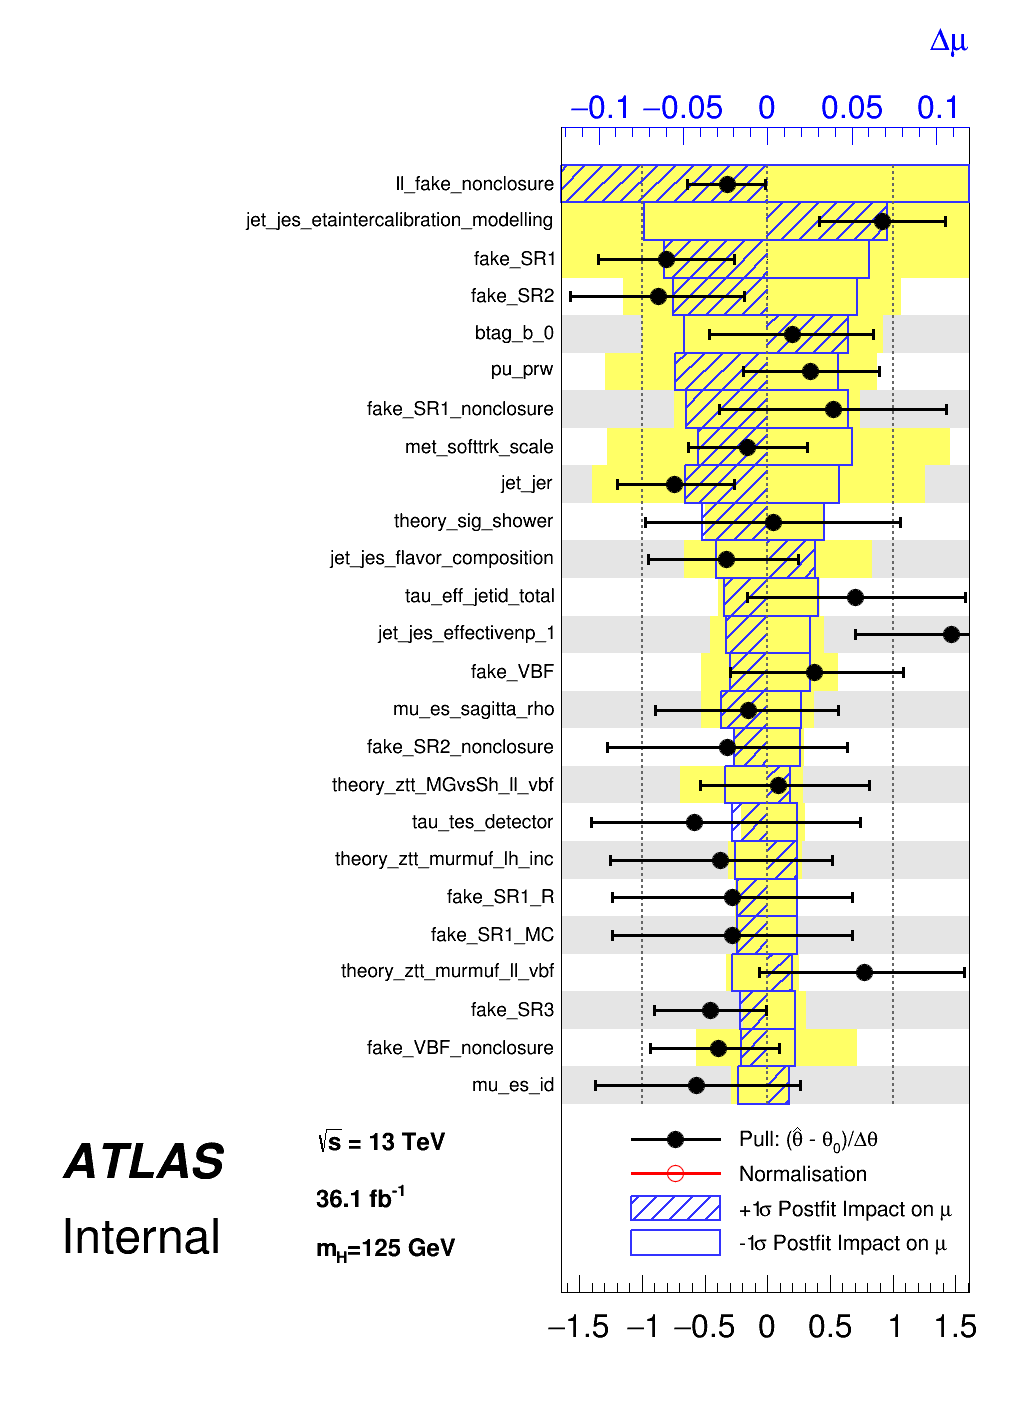
\includegraphics[width=.50\textwidth,height=.70\textheight,type=pdf,ext=.pdf,read=.pdf]{/afs/cern.ch/user/a/atpathak/afswork/public/WSMaker/pdf-files/version/comb_mtau_cba_pulls_125}
%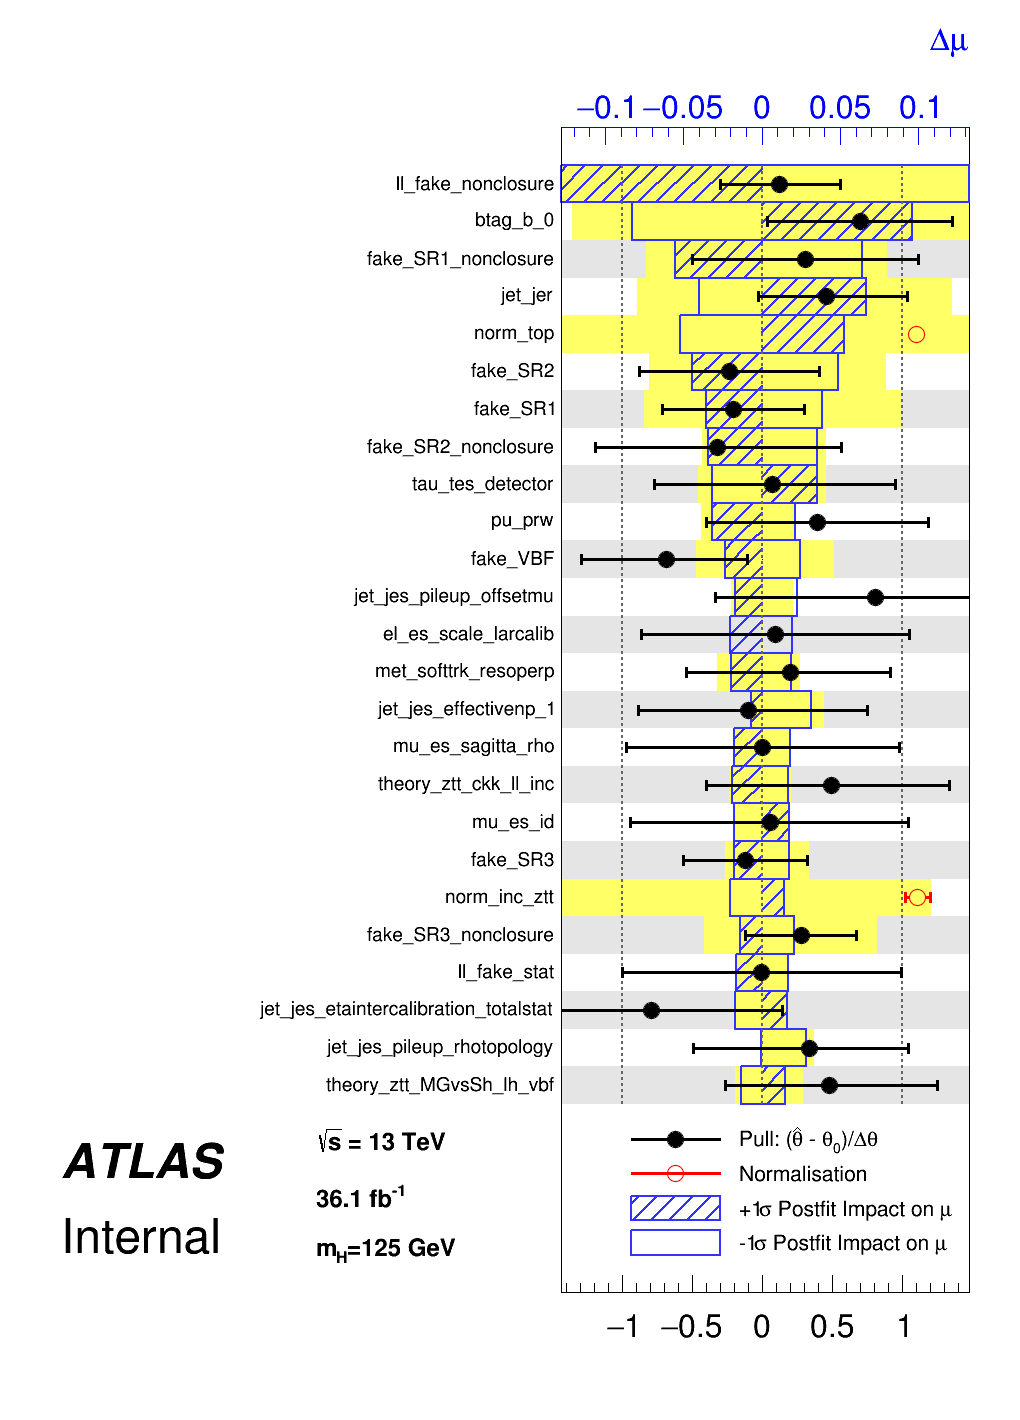
\includegraphics[width=.50\textwidth,height=.70\textheight,type=pdf,ext=.pdf,read=.pdf]{/afs/cern.ch/user/a/atpathak/afswork/public/WSMaker/pdf-files/version/comb_etau_cba_pulls_125}
%\end{normalsize}
%\end{frame}
%-----------------------------------------------
%\begin{frame}
%\frametitle{NP Ranking for combined ll+lh(MVA)}
%\begin{normalsize}
%\hspace{1.2in} $\mu\tau_{had}$
%\hspace{1.5in}$e\tau_{had}$
%\vspace*{0.2cm}
%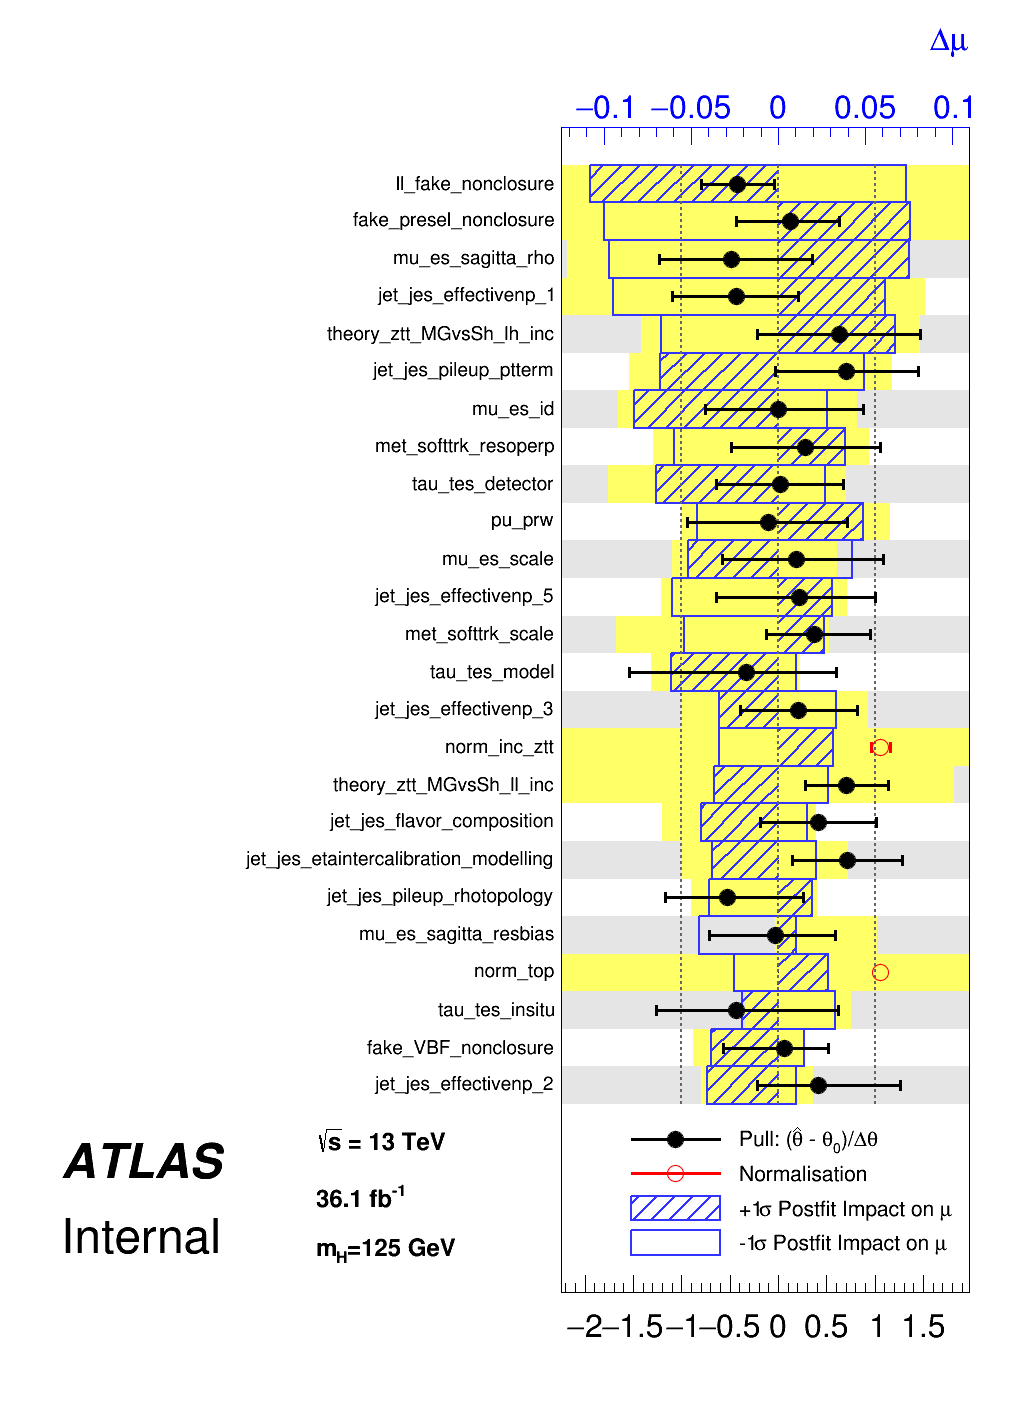
\includegraphics[width=.50\textwidth,height=.70\textheight,type=pdf,ext=.pdf,read=.pdf]{/afs/cern.ch/user/a/atpathak/afswork/public/WSMaker/pdf-files/version/comb_mtau_mva_pulls_125}
%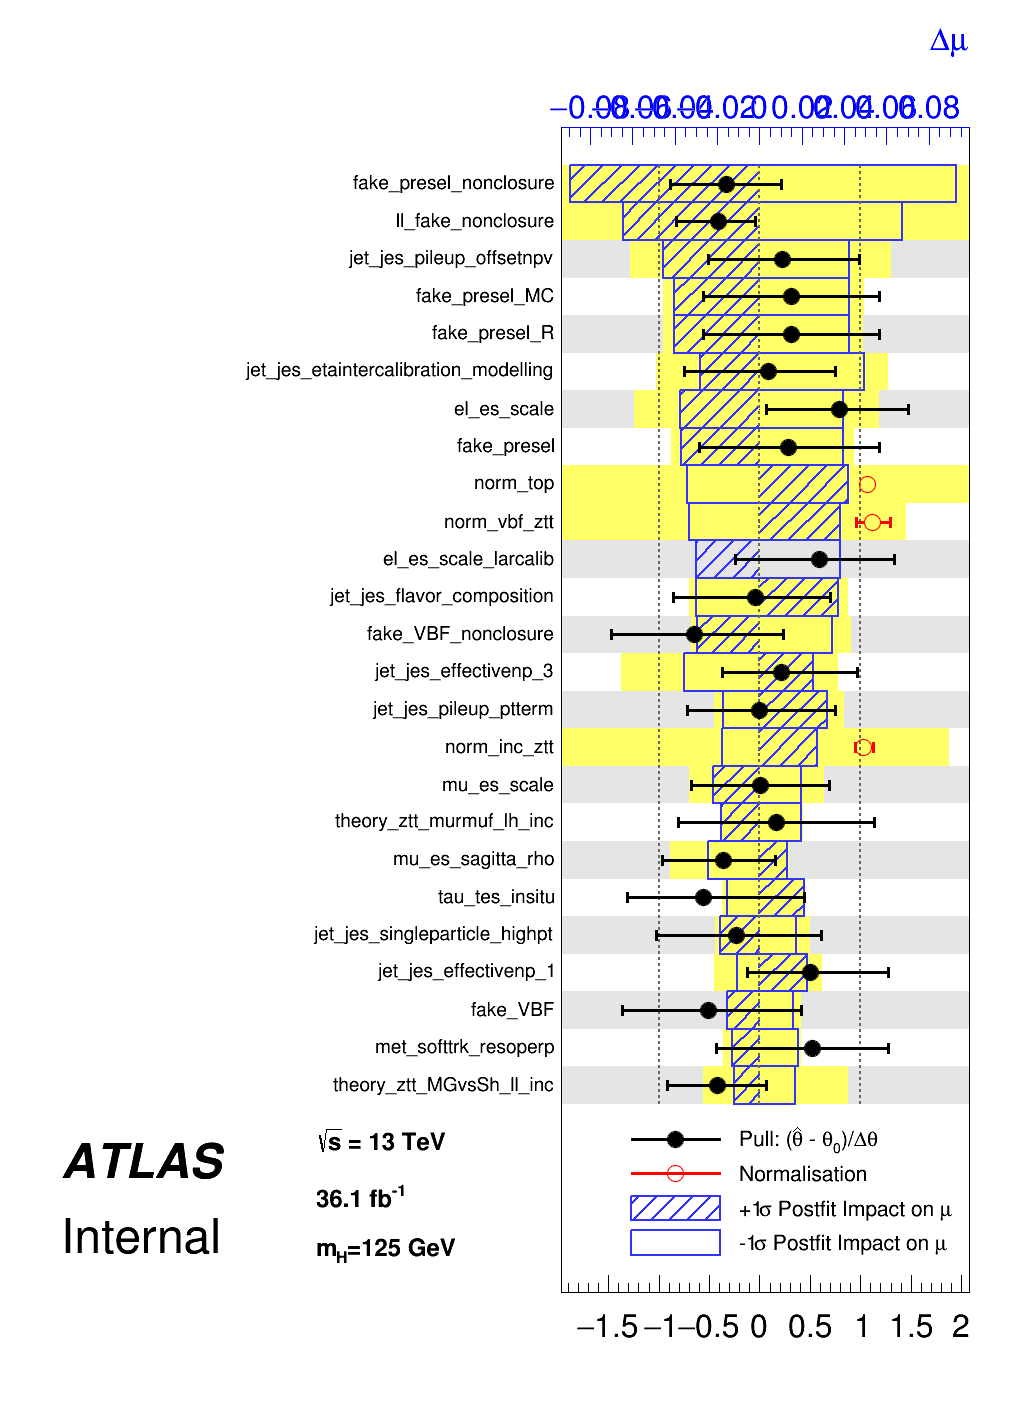
\includegraphics[width=.50\textwidth,height=.70\textheight,type=pdf,ext=.pdf,read=.pdf]{/afs/cern.ch/user/a/atpathak/afswork/public/WSMaker/pdf-files/version/comb_etau_mva_pulls_125}
%\end{normalsize}
%\end{frame}
%-----------------------------------------------
\begin{frame}
\frametitle{NP Ranking for combined ll+lh(CBA) for $\mu\tau_{had}$}
\begin{normalsize}
\hspace{1.2in} Atanu
\hspace{1.5in} Julia
\vspace*{0.2cm}
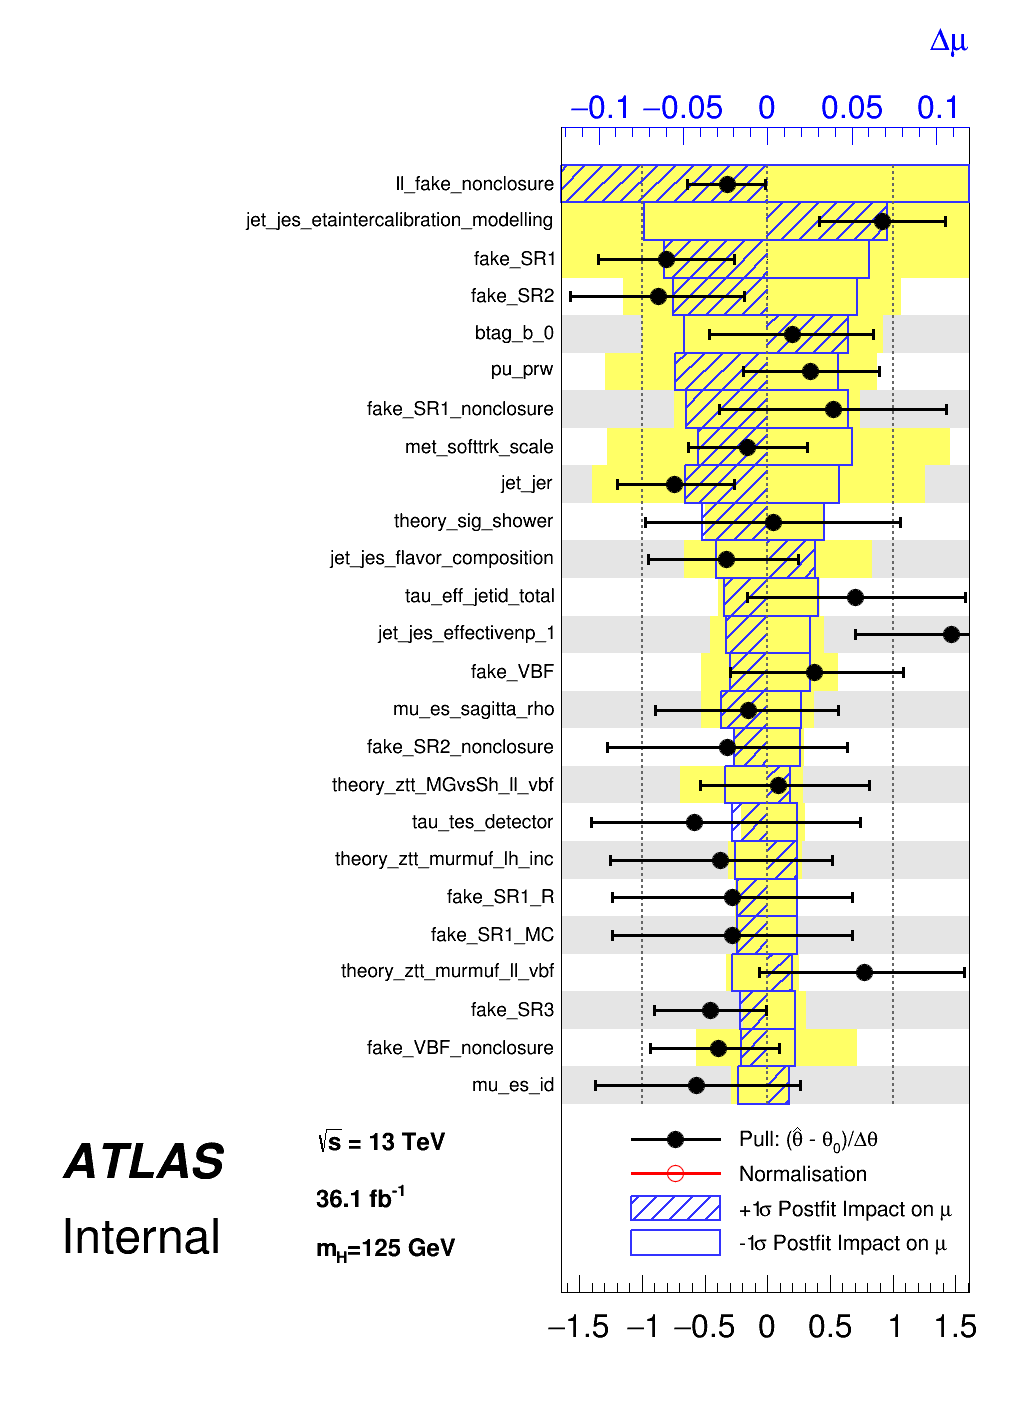
\includegraphics[width=.50\textwidth,height=.70\textheight,type=pdf,ext=.pdf,read=.pdf]{/afs/cern.ch/user/a/atpathak/afswork/public/WSMaker/pdf-files/version/comb_mtau_cba_pulls_125}
\includegraphics[width=.50\textwidth,height=.70\textheight,type=pdf,ext=.pdf,read=.pdf]{/afs/cern.ch/user/a/atpathak/afswork/public/Pixel/LFV_Plots/NPranking0826/Bigjob.combmtaucba_job50of50_LFVlh_13TeV_combmtaucba_Systs_125_pulls_125}
\end{normalsize}
\end{frame}
%-----------------------------------------------
\begin{frame}
\frametitle{NP Ranking for combined ll+lh(CBA) for $e\tau_{had}$}
\begin{normalsize}
\hspace{1.2in} Atanu
\hspace{1.5in} Julia
\vspace*{0.2cm}
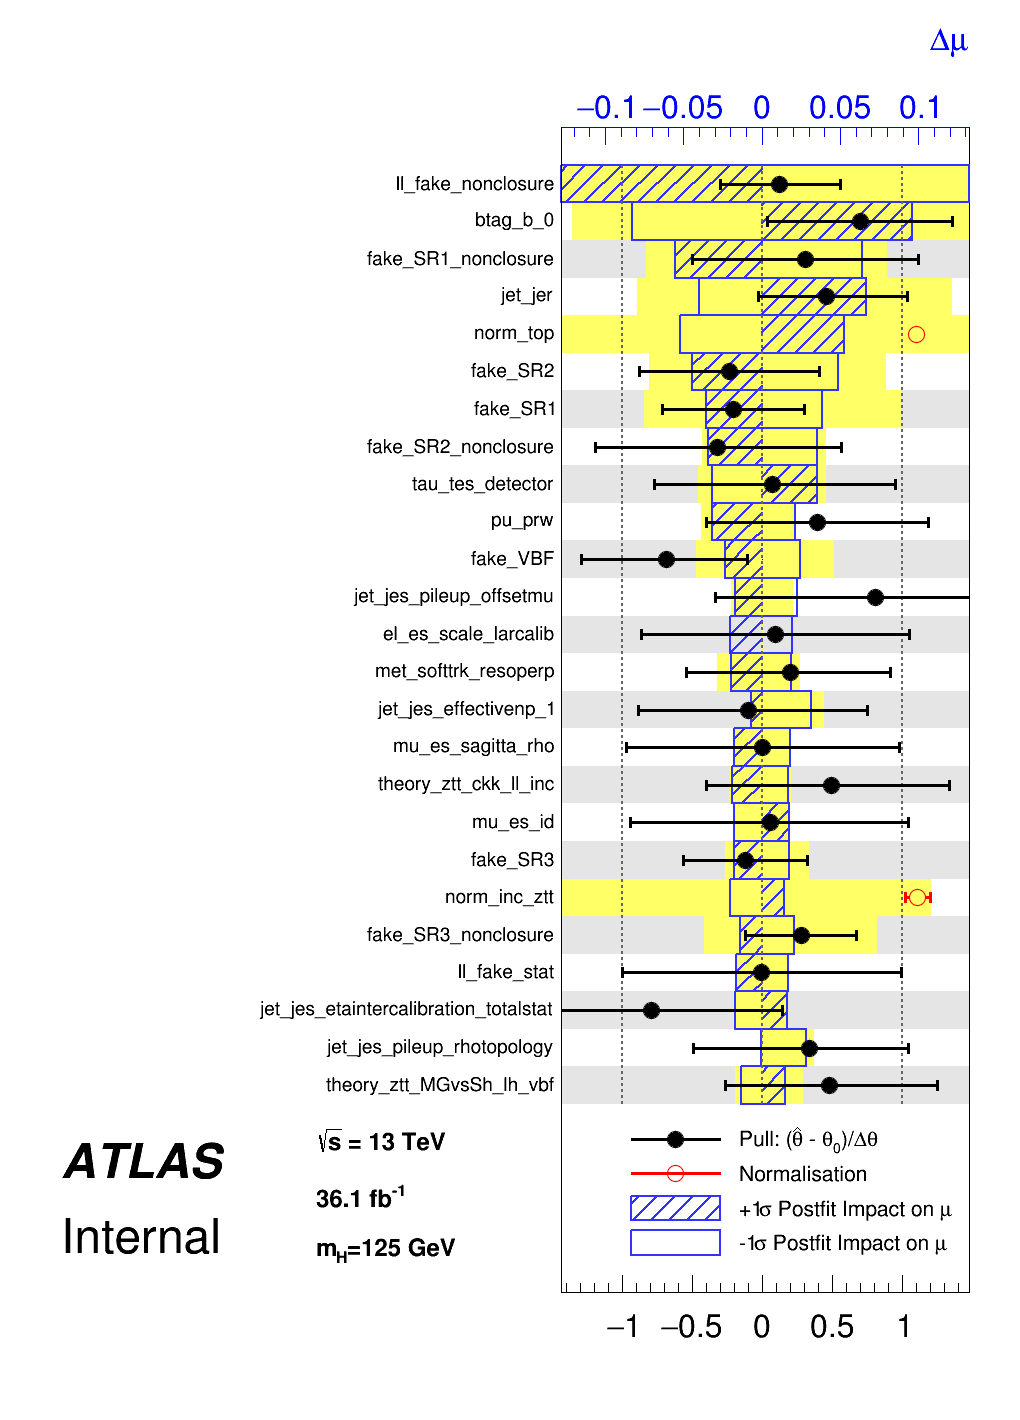
\includegraphics[width=.50\textwidth,height=.70\textheight,type=pdf,ext=.pdf,read=.pdf]{/afs/cern.ch/user/a/atpathak/afswork/public/WSMaker/pdf-files/version/comb_etau_cba_pulls_125}
\includegraphics[width=.50\textwidth,height=.70\textheight,type=pdf,ext=.pdf,read=.pdf]{/afs/cern.ch/user/a/atpathak/afswork/public/Pixel/LFV_Plots/NPranking0826/Bigjob.combetaucba_job50of50_LFVlh_13TeV_combetaucba_Systs_125_pulls_125}
\end{normalsize}
\end{frame}
%-----------------------------------------------
\begin{frame}
\frametitle{NP Ranking for combined ll+lh(MVA) for $\mu\tau_{had}$}
\begin{normalsize}
\hspace{1.2in} Atanu
\hspace{1.5in} Julia
\vspace*{0.2cm}
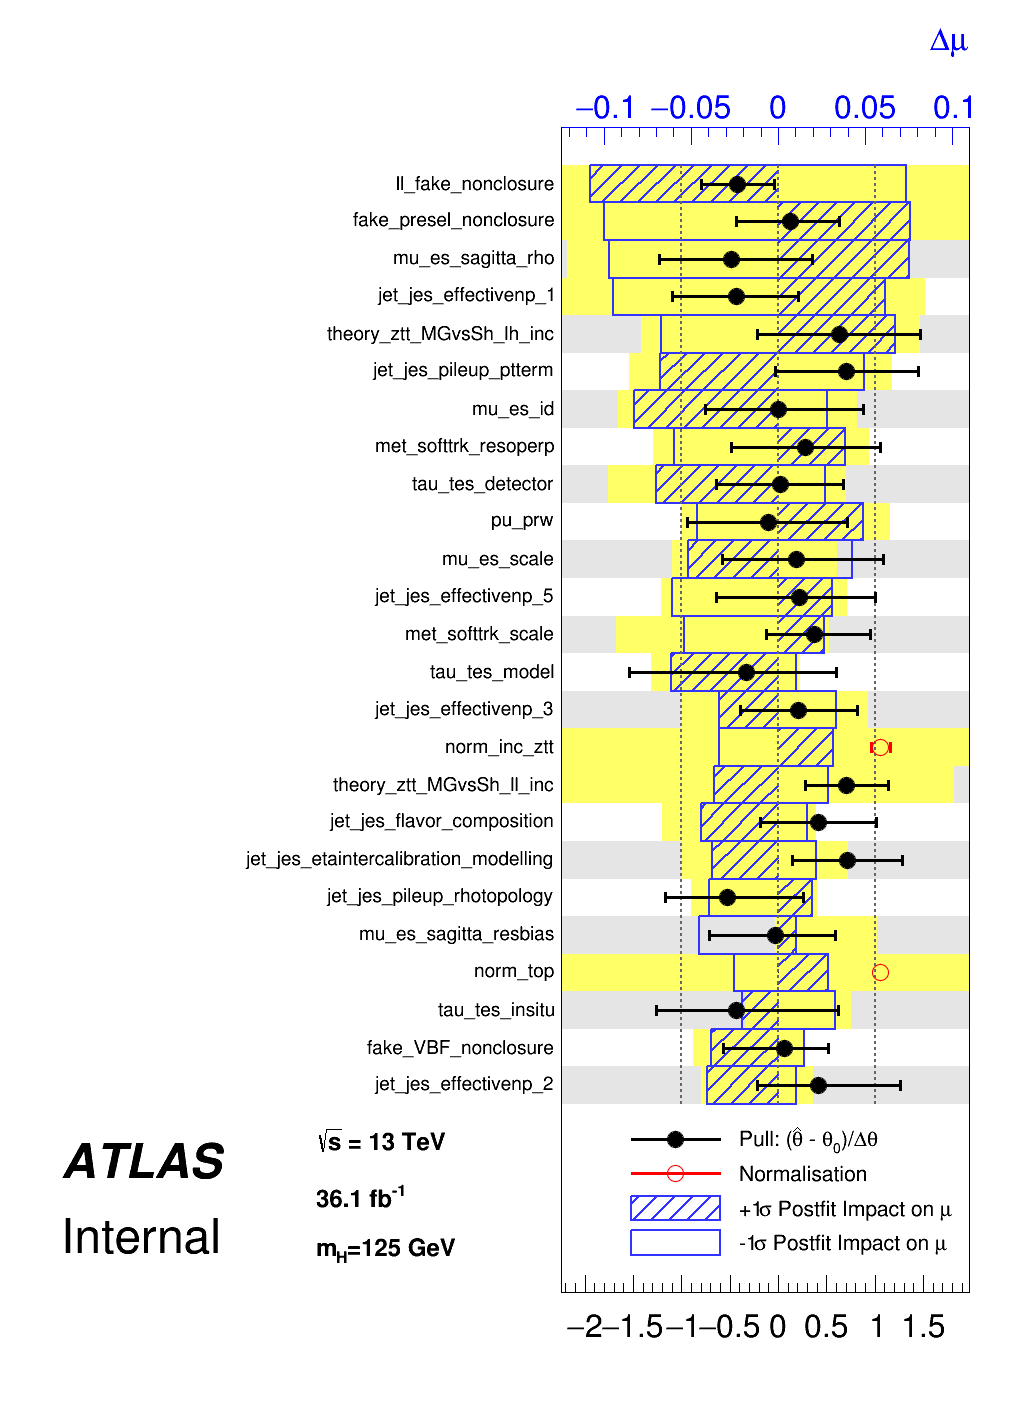
\includegraphics[width=.50\textwidth,height=.70\textheight,type=pdf,ext=.pdf,read=.pdf]{/afs/cern.ch/user/a/atpathak/afswork/public/WSMaker/pdf-files/version/comb_mtau_mva_pulls_125}
\includegraphics[width=.50\textwidth,height=.70\textheight,type=pdf,ext=.pdf,read=.pdf]{/afs/cern.ch/user/a/atpathak/afswork/public/Pixel/LFV_Plots/NPranking0826/Bigjob.combmtaumva_job50of50_LFVlh_13TeV_combmtaumva_Systs_125_pulls_125}
\end{normalsize}
\end{frame}
%-----------------------------------------------
\begin{frame}
\frametitle{NP Ranking for combined ll+lh(MVA) for $e\tau_{had}$}
\begin{normalsize}
\hspace{1.2in} Atanu
\hspace{1.5in} Julia
\vspace*{0.2cm}
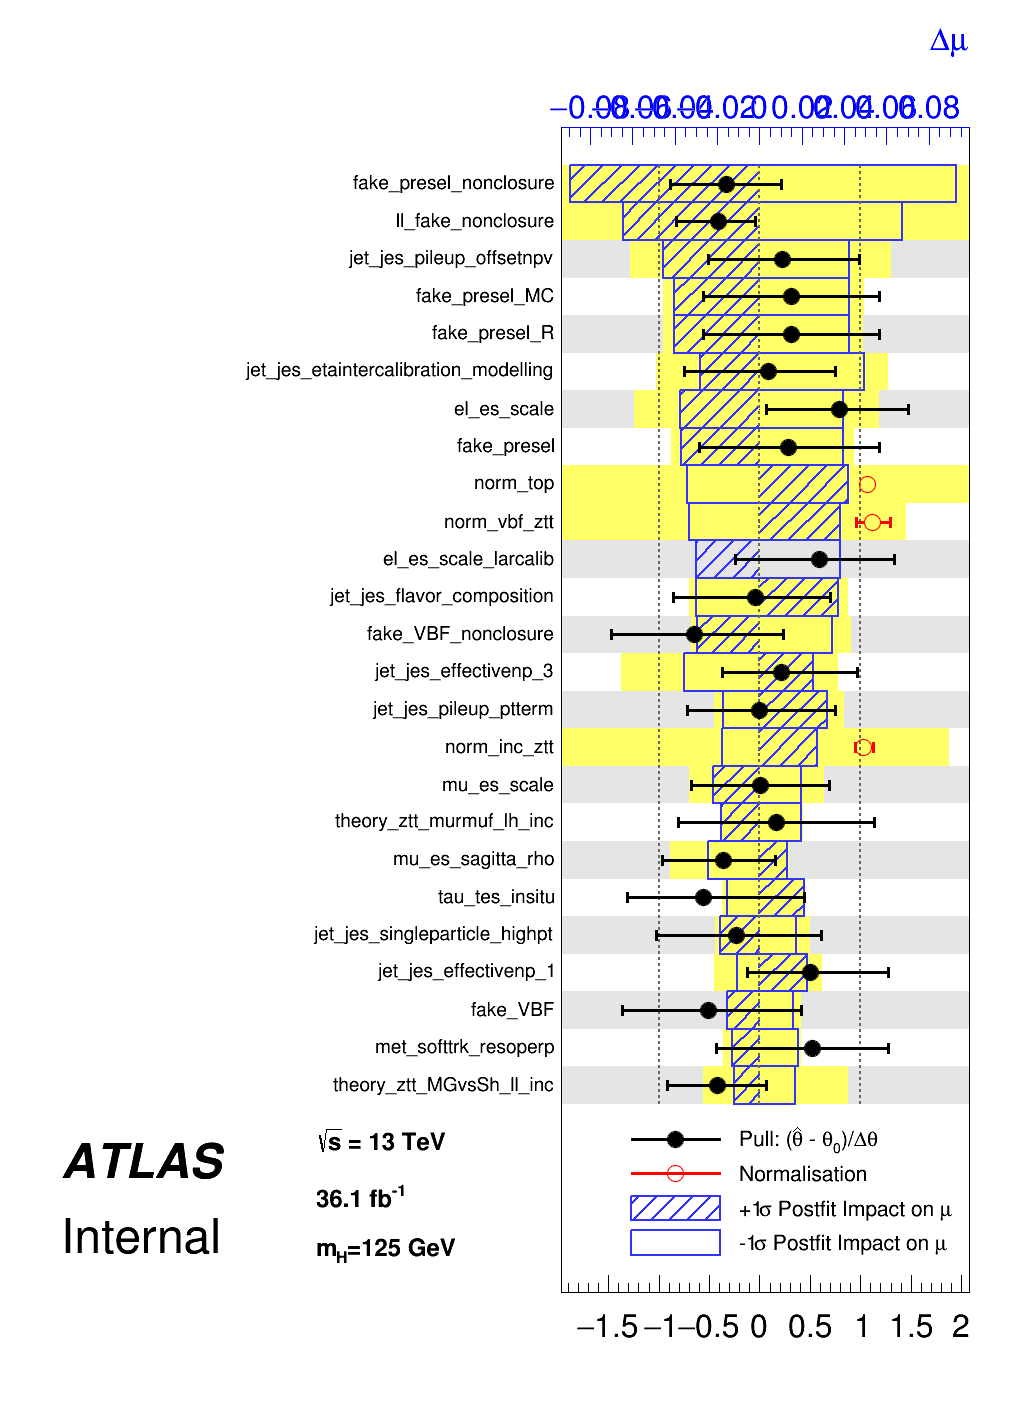
\includegraphics[width=.50\textwidth,height=.70\textheight,type=pdf,ext=.pdf,read=.pdf]{/afs/cern.ch/user/a/atpathak/afswork/public/WSMaker/pdf-files/version/comb_etau_mva_pulls_125}
\includegraphics[width=.50\textwidth,height=.70\textheight,type=pdf,ext=.pdf,read=.pdf]{/afs/cern.ch/user/a/atpathak/afswork/public/Pixel/LFV_Plots/NPranking0826/Bigjob.combetaumva_job50of50_LFVlh_13TeV_combetaumva_Systs_125_pulls_125}
\end{normalsize}
\end{frame}
%-----------------------------------------------
\end{document}
%-----------------------------------------------
\begin{frame}
\frametitle{Postfit plots for combined ll+lh for mtau(CBA)}
\begin{normalsize}
%$\mu\tau_{had}$(top) and \hspace{0.1in}  $e\tau_{had}$(ddZll)(bottom)
\vspace*{0.5cm}
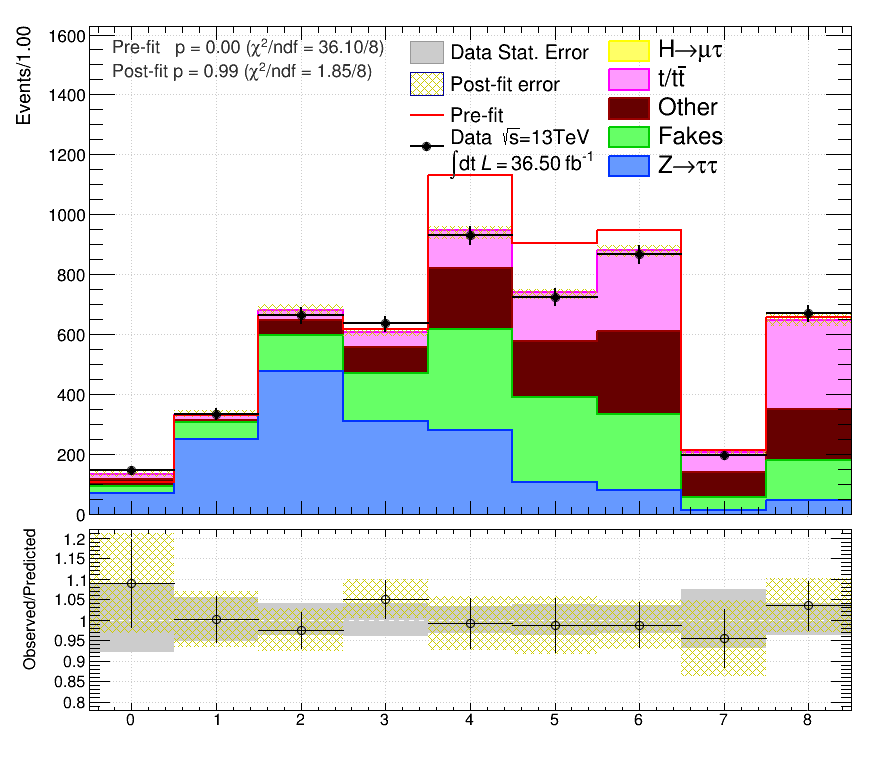
\includegraphics[width=.25\textwidth,height=.30\textheight,type=pdf,ext=.png,read=.png]{/afs/cern.ch/work/a/atpathak/public/FitBox/plots/MColl_me_inc_regsig_selCBA_}
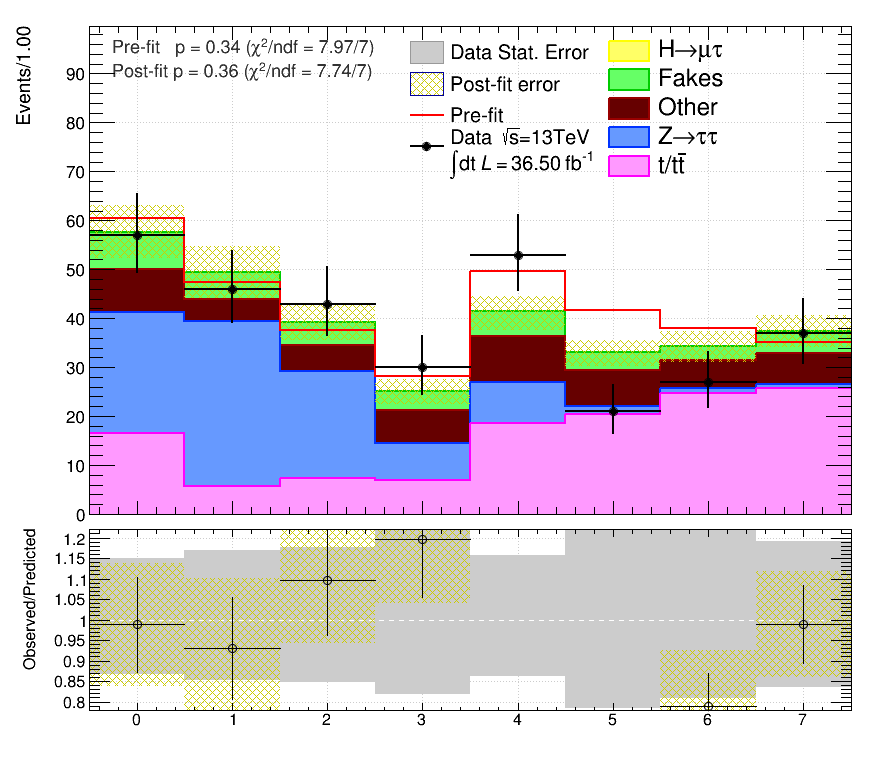
\includegraphics[width=.25\textwidth,height=.30\textheight,type=pdf,ext=.png,read=.png]{/afs/cern.ch/work/a/atpathak/public/FitBox/plots/MColl_me_vbf_regsig_selCBA_}\\
\hspace{0.5in}ll\_inc 
\hspace{0.75in}ll\_vbf\\
\vspace*{0.5cm}
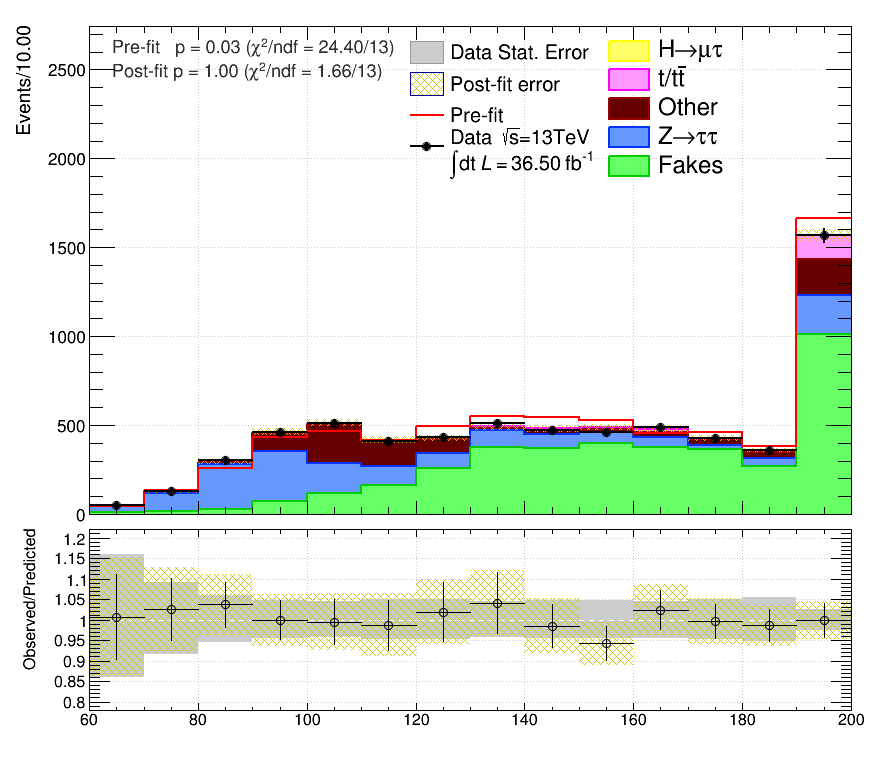
\includegraphics[width=.25\textwidth,height=.30\textheight,type=pdf,ext=.png,read=.png]{/afs/cern.ch/work/a/atpathak/public/FitBox/plots/MColl_mtau_inc1_regsig_selCBA_}
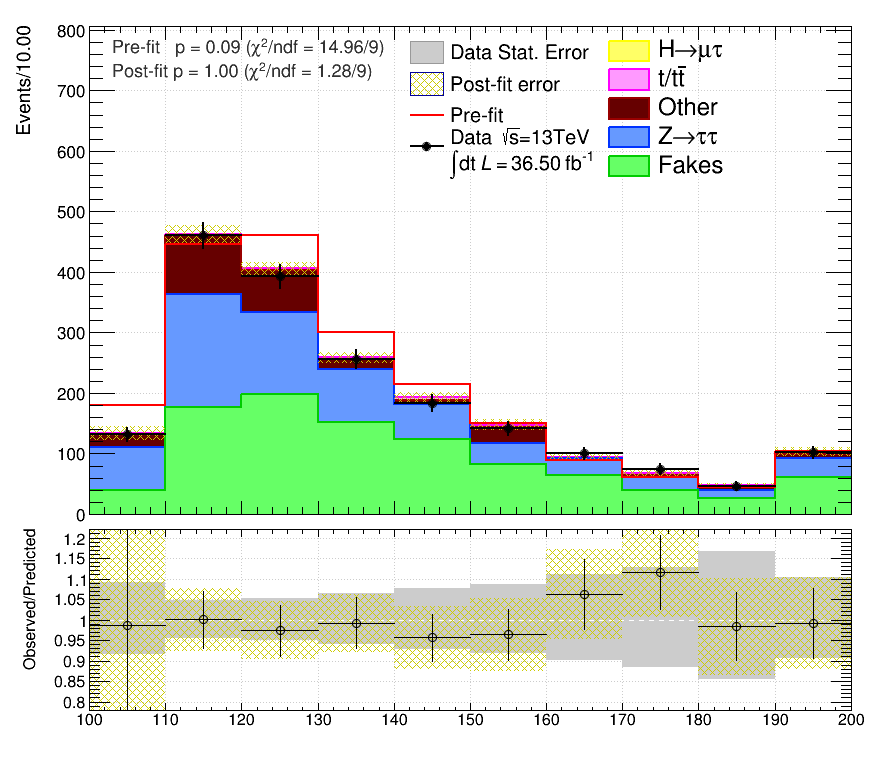
\includegraphics[width=.25\textwidth,height=.30\textheight,type=pdf,ext=.png,read=.png]{/afs/cern.ch/work/a/atpathak/public/FitBox/plots/MColl_mtau_inc2_regsig_selCBA_}
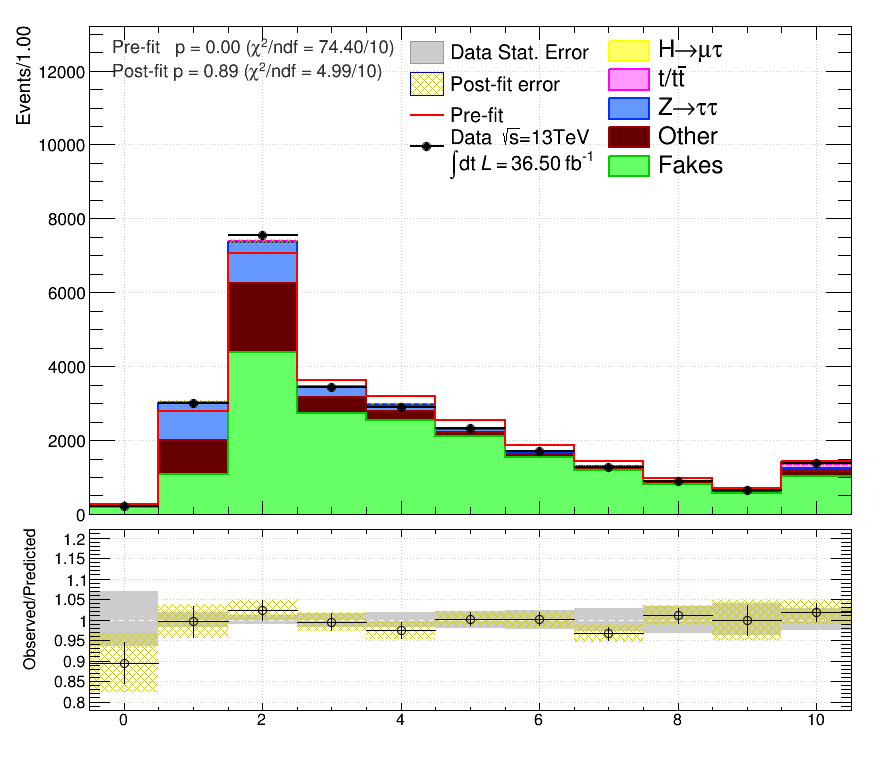
\includegraphics[width=.25\textwidth,height=.30\textheight,type=pdf,ext=.png,read=.png]{/afs/cern.ch/work/a/atpathak/public/FitBox/plots/MColl_mtau_inc3_regsig_selCBA_}
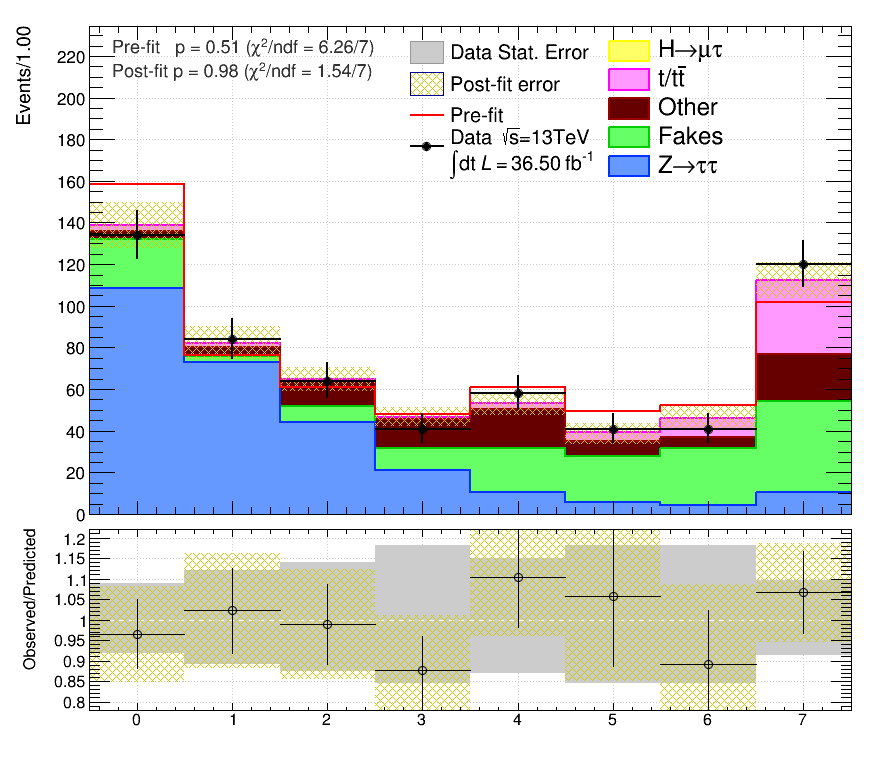
\includegraphics[width=.25\textwidth,height=.30\textheight,type=pdf,ext=.png,read=.png]{/afs/cern.ch/work/a/atpathak/public/FitBox/plots/MColl_mtau_vbf_regsig_selCBA_}\\
\hspace{0.3in}lh\_inc1 
\hspace{0.55in}lh\_inc2
\hspace{0.55in}lh\_inc3
\hspace{0.55in}lh\_VBF
\end{normalsize}
\end{frame}
%-----------------------------------------------
\begin{frame}
\frametitle{Postfit plots for combined ll+lh for etau(CBA)}
\begin{normalsize}
%$\mu\tau_{had}$(top) and \hspace{0.1in}  $e\tau_{had}$(ddZll)(bottom)
\vspace*{0.5cm}
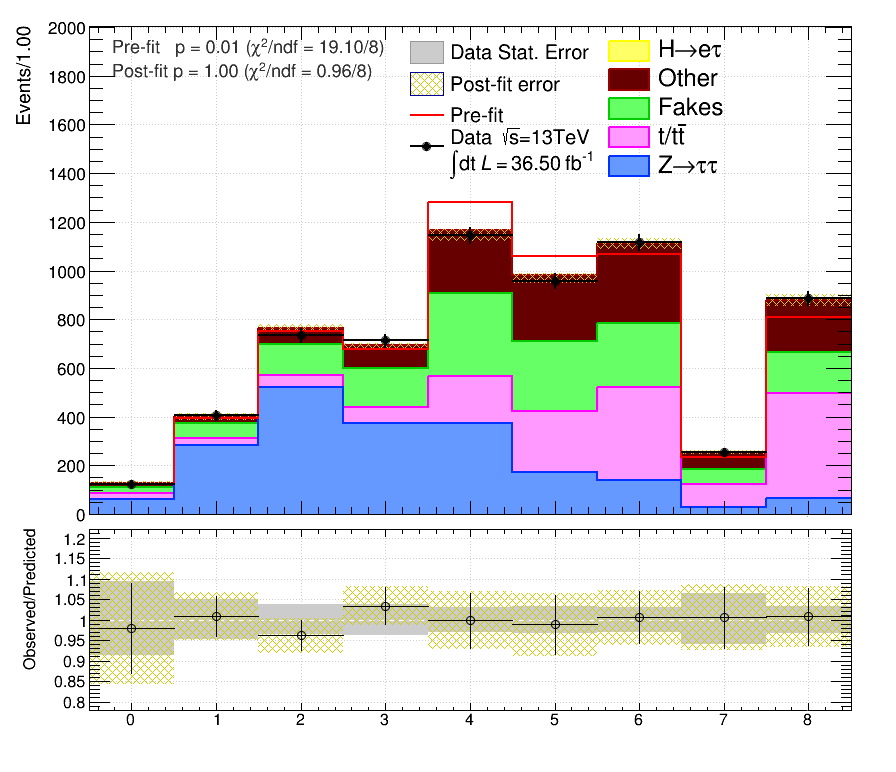
\includegraphics[width=.25\textwidth,height=.30\textheight,type=pdf,ext=.png,read=.png]{/afs/cern.ch/work/a/atpathak/public/FitBox/plots/MColl_em_inc_regsig_selCBA_}
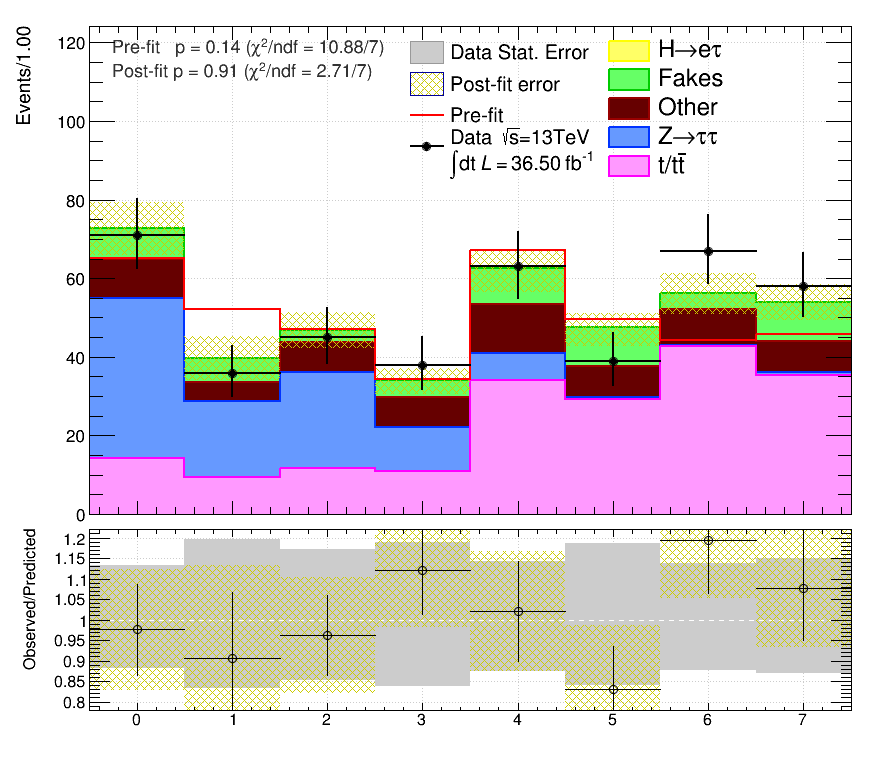
\includegraphics[width=.25\textwidth,height=.30\textheight,type=pdf,ext=.png,read=.png]{/afs/cern.ch/work/a/atpathak/public/FitBox/plots/MColl_em_vbf_regsig_selCBA_}\\
\hspace{0.5in}ll\_inc 
\hspace{0.75in}ll\_vbf\\
\vspace*{0.5cm}
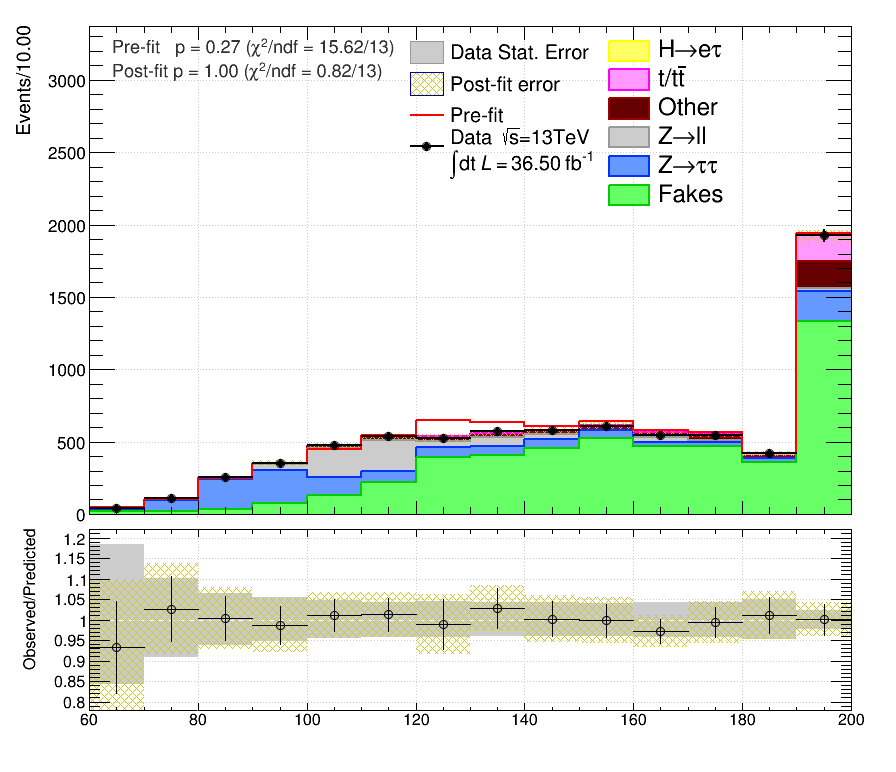
\includegraphics[width=.25\textwidth,height=.30\textheight,type=pdf,ext=.png,read=.png]{/afs/cern.ch/work/a/atpathak/public/FitBox/plots/MColl_etau_inc1_regsig_selCBA_}
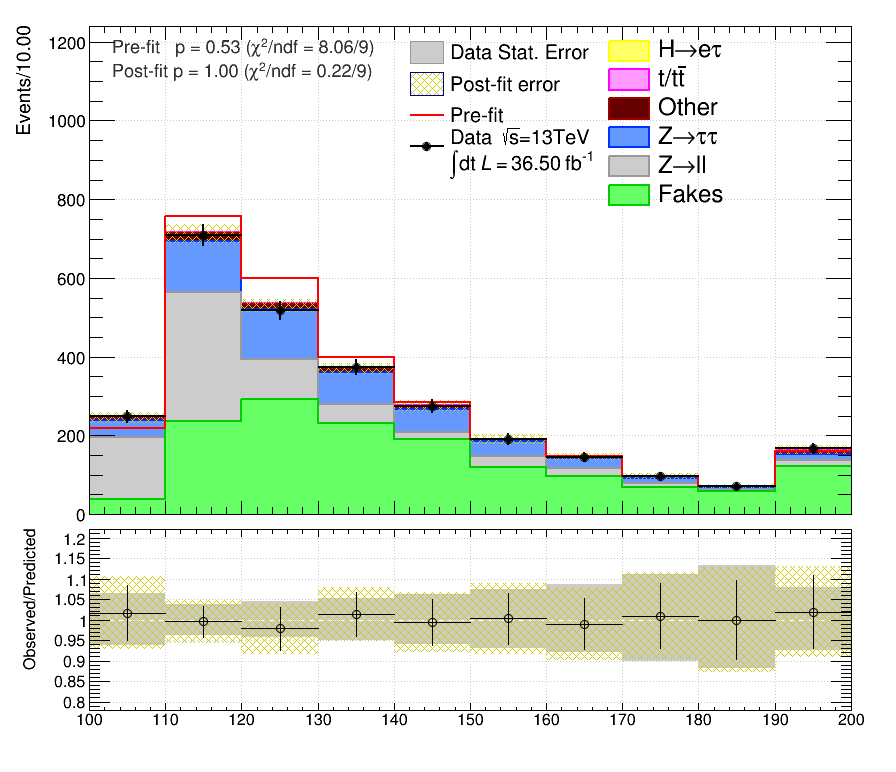
\includegraphics[width=.25\textwidth,height=.30\textheight,type=pdf,ext=.png,read=.png]{/afs/cern.ch/work/a/atpathak/public/FitBox/plots/MColl_etau_inc2_regsig_selCBA_}
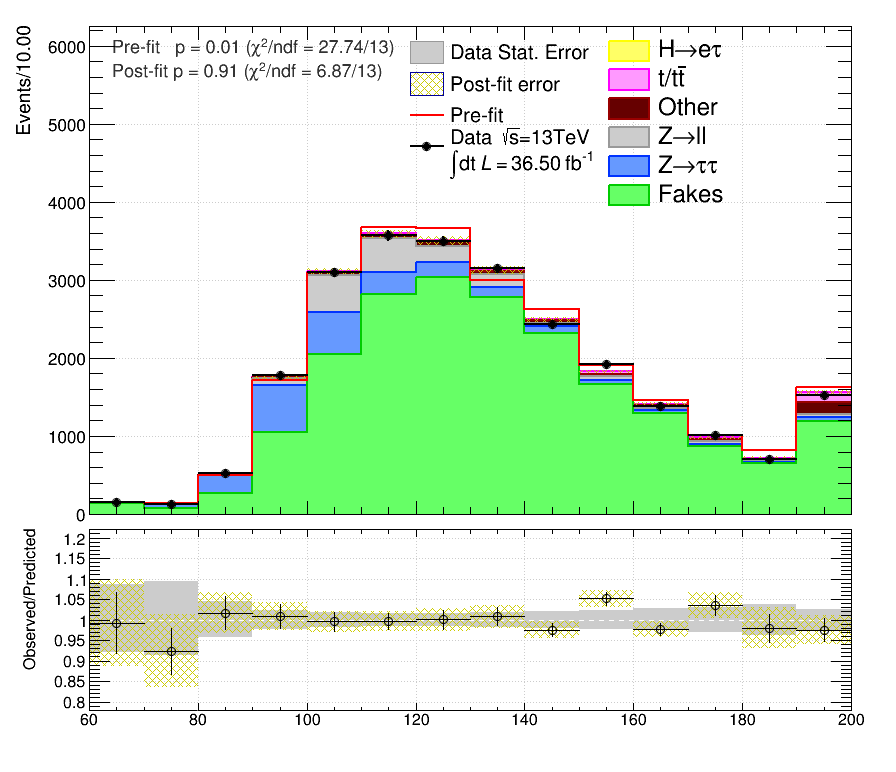
\includegraphics[width=.25\textwidth,height=.30\textheight,type=pdf,ext=.png,read=.png]{/afs/cern.ch/work/a/atpathak/public/FitBox/plots/MColl_etau_inc3_regsig_selCBA_}
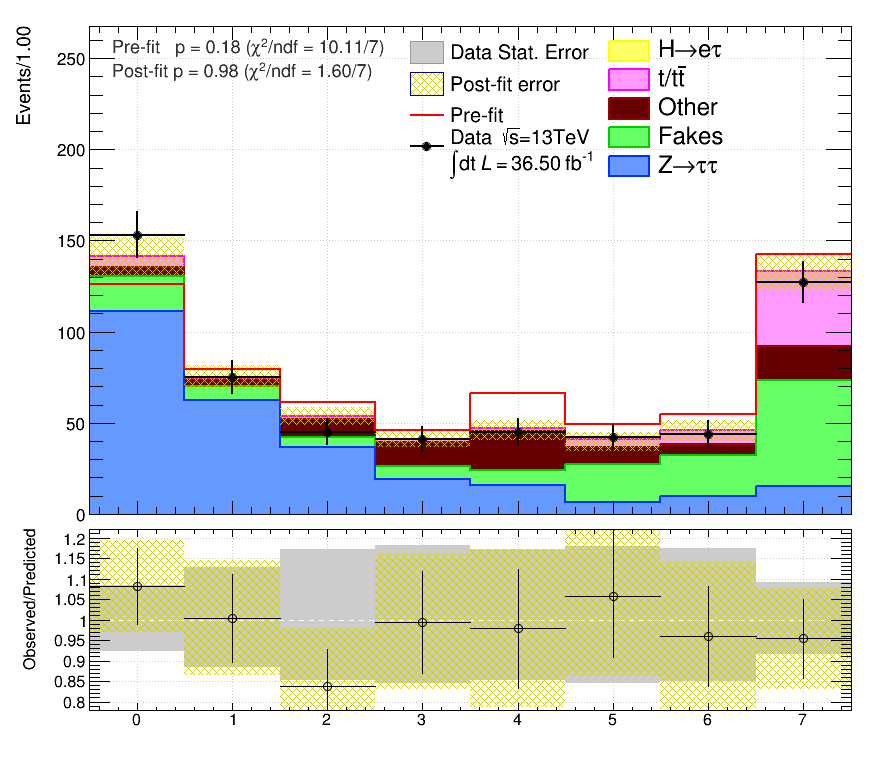
\includegraphics[width=.25\textwidth,height=.30\textheight,type=pdf,ext=.png,read=.png]{/afs/cern.ch/work/a/atpathak/public/FitBox/plots/MColl_etau_vbf_regsig_selCBA_}\\
\hspace{0.3in}lh\_inc1 
\hspace{0.55in}lh\_inc2
\hspace{0.55in}lh\_inc3
\hspace{0.55in}lh\_VBF
\end{normalsize}
\end{frame}
%-----------------------------------------------
\begin{frame}
\frametitle{Postfit plots for combined ll+lh for MVA }
\begin{normalsize}
%$\mu\tau_{had}$(top) and \hspace{0.1in}  $e\tau_{had}$(ddZll)(bottom)
\vspace*{0.5cm}
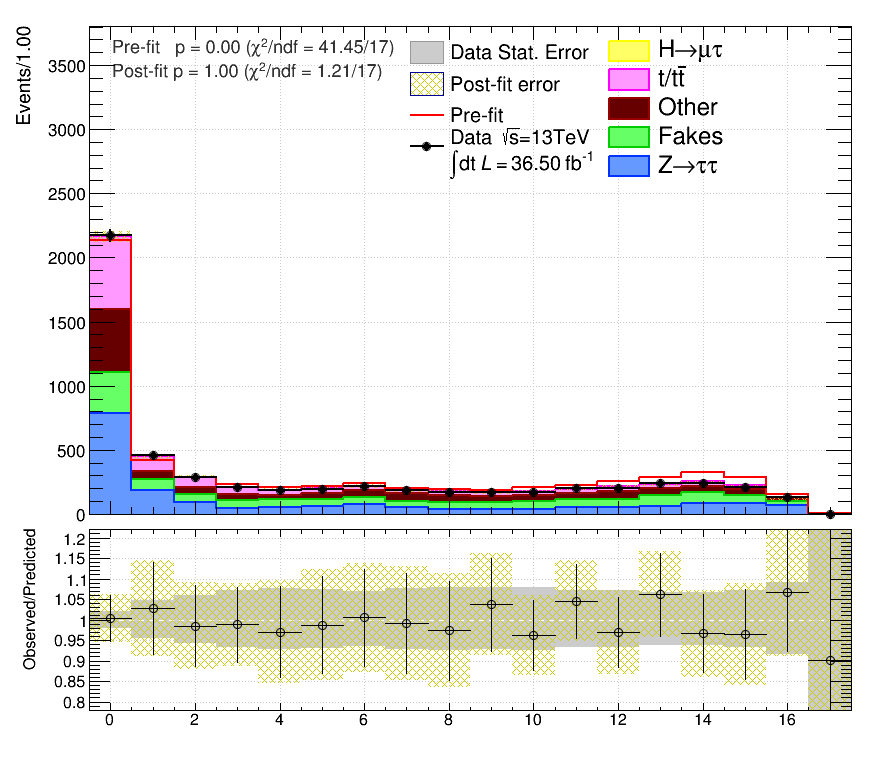
\includegraphics[width=.25\textwidth,height=.30\textheight,type=pdf,ext=.png,read=.png]{/afs/cern.ch/work/a/atpathak/public/FitBox/plots/MMC_me_inc_regsig_selMVA_liner}
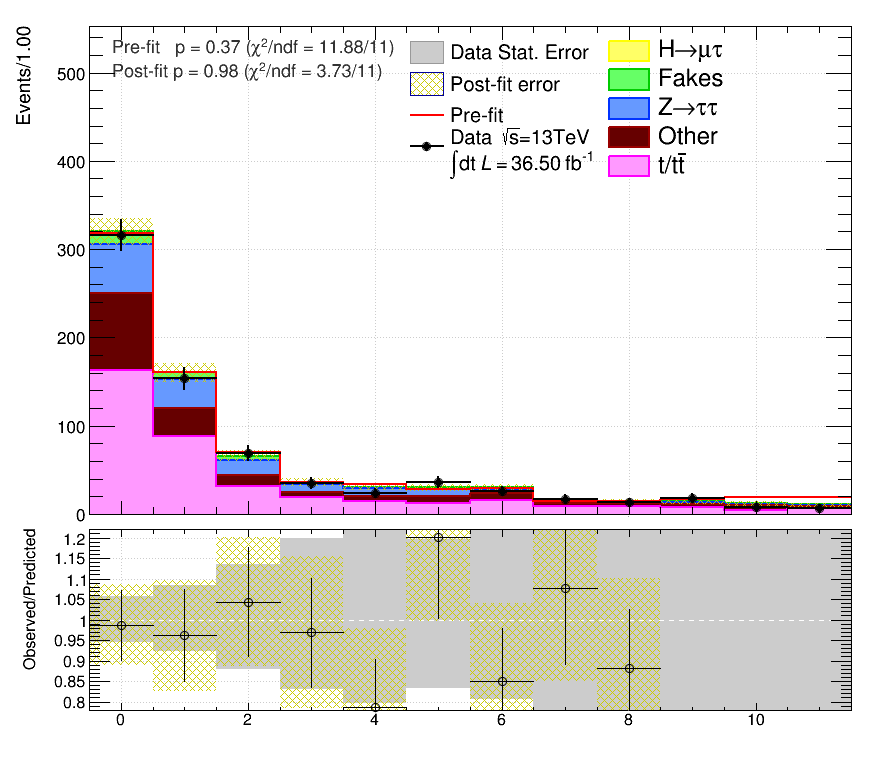
\includegraphics[width=.25\textwidth,height=.30\textheight,type=pdf,ext=.png,read=.png]{/afs/cern.ch/work/a/atpathak/public/FitBox/plots/MMC_me_vbf_regsig_selMVA_liner}
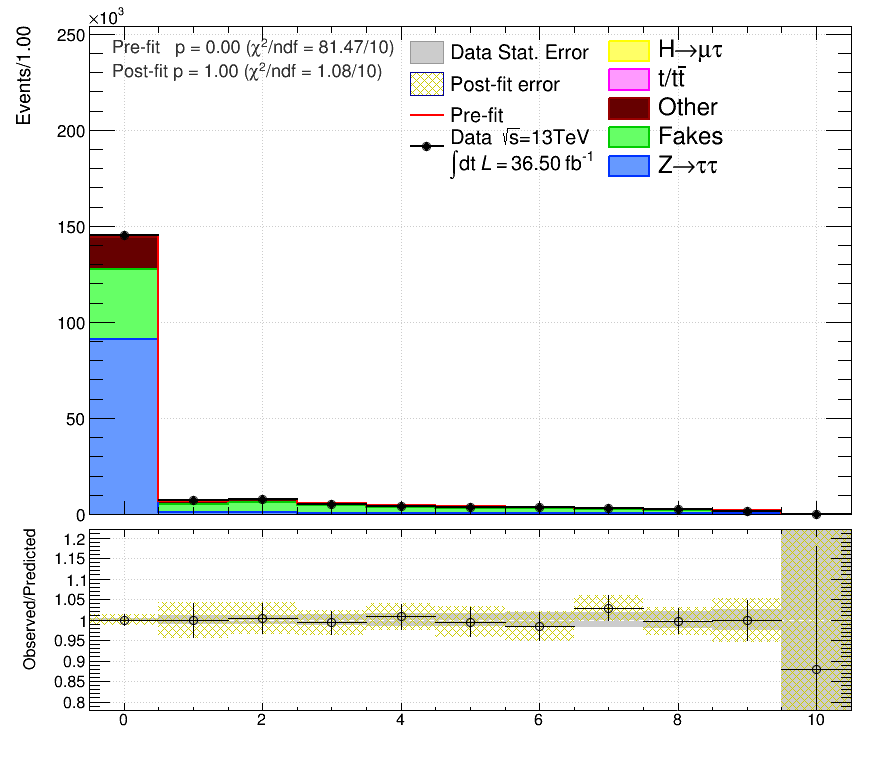
\includegraphics[width=.25\textwidth,height=.30\textheight,type=pdf,ext=.png,read=.png]{/afs/cern.ch/work/a/atpathak/public/FitBox/plots/MMC_mtau_inc_regsig_selMVA_liner}
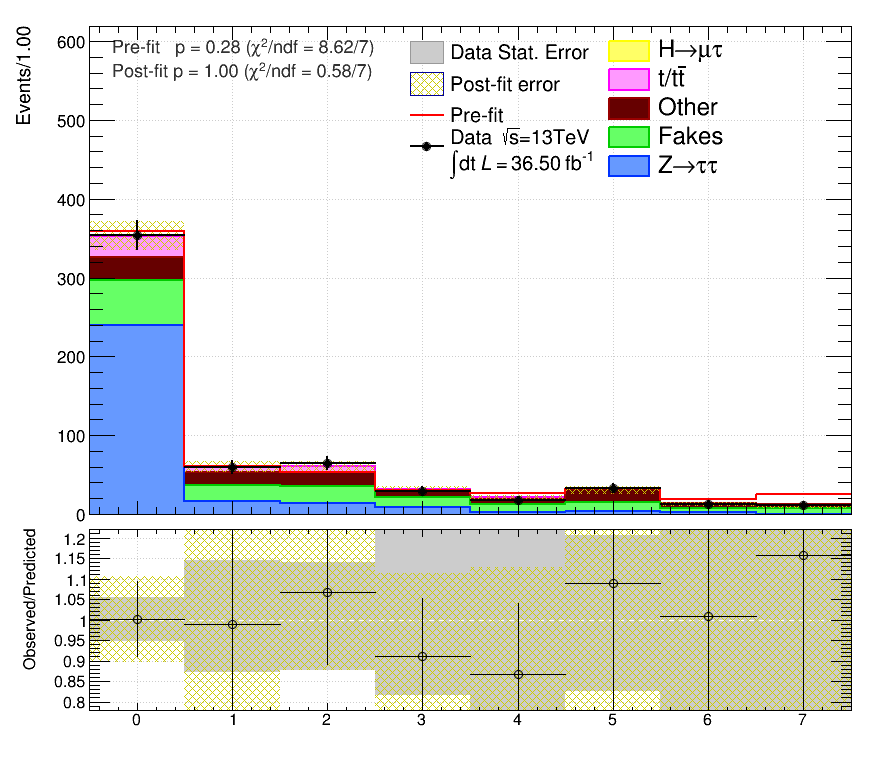
\includegraphics[width=.25\textwidth,height=.30\textheight,type=pdf,ext=.png,read=.png]{/afs/cern.ch/work/a/atpathak/public/FitBox/plots/MMC_mtau_vbf_regsig_selMVA_liner}\\
\vspace*{0.5cm}
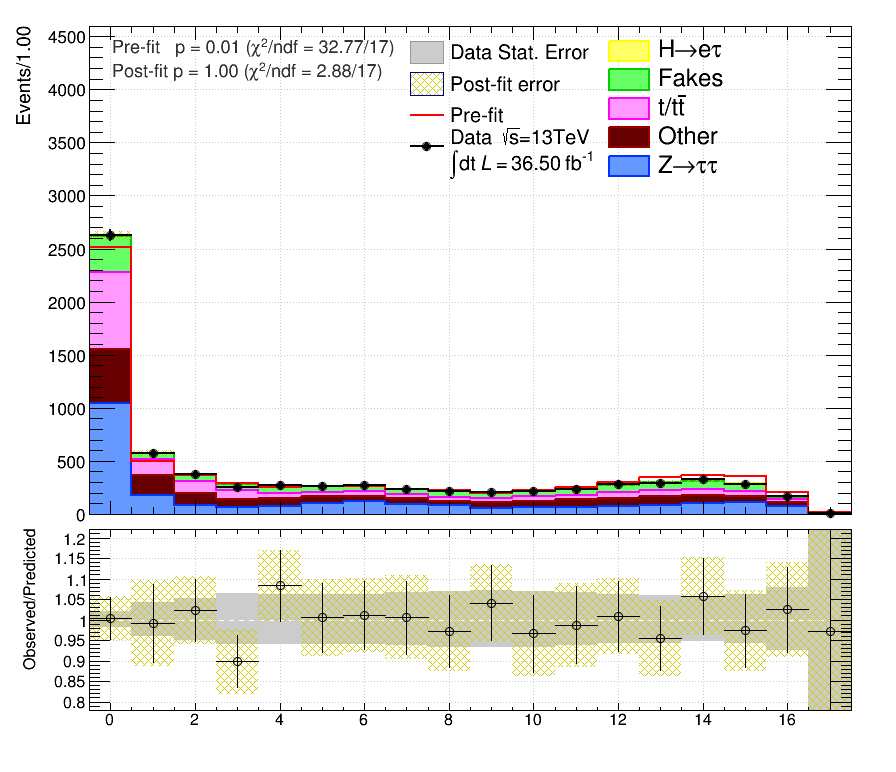
\includegraphics[width=.25\textwidth,height=.30\textheight,type=pdf,ext=.png,read=.png]{/afs/cern.ch/work/a/atpathak/public/FitBox/plots/MMC_em_inc_regsig_selMVA_liner}
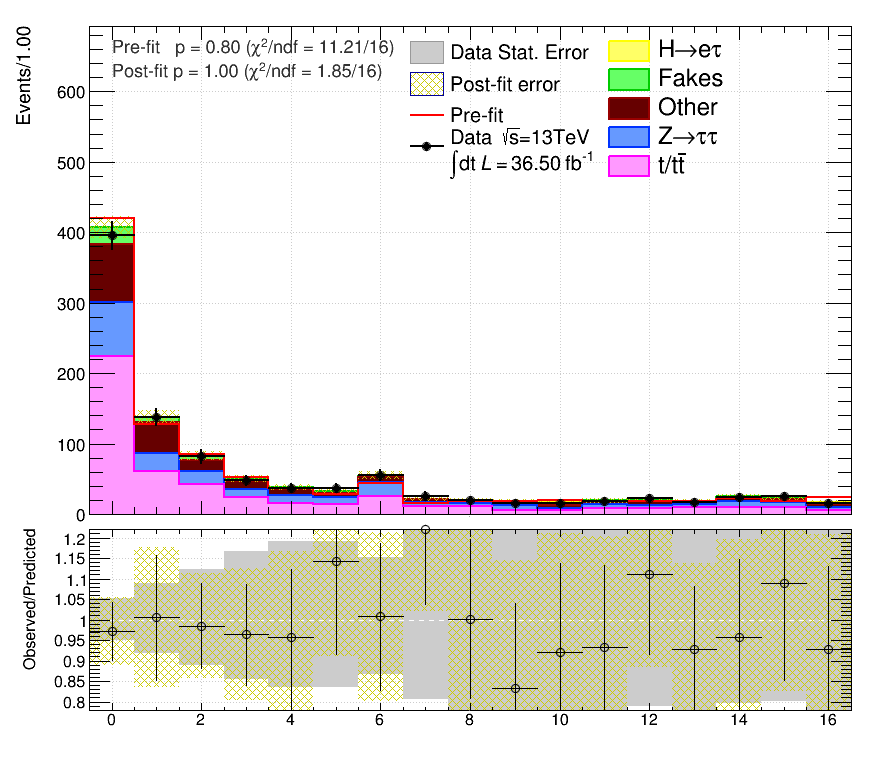
\includegraphics[width=.25\textwidth,height=.30\textheight,type=pdf,ext=.png,read=.png]{/afs/cern.ch/work/a/atpathak/public/FitBox/plots/MMC_em_vbf_regsig_selMVA_liner}
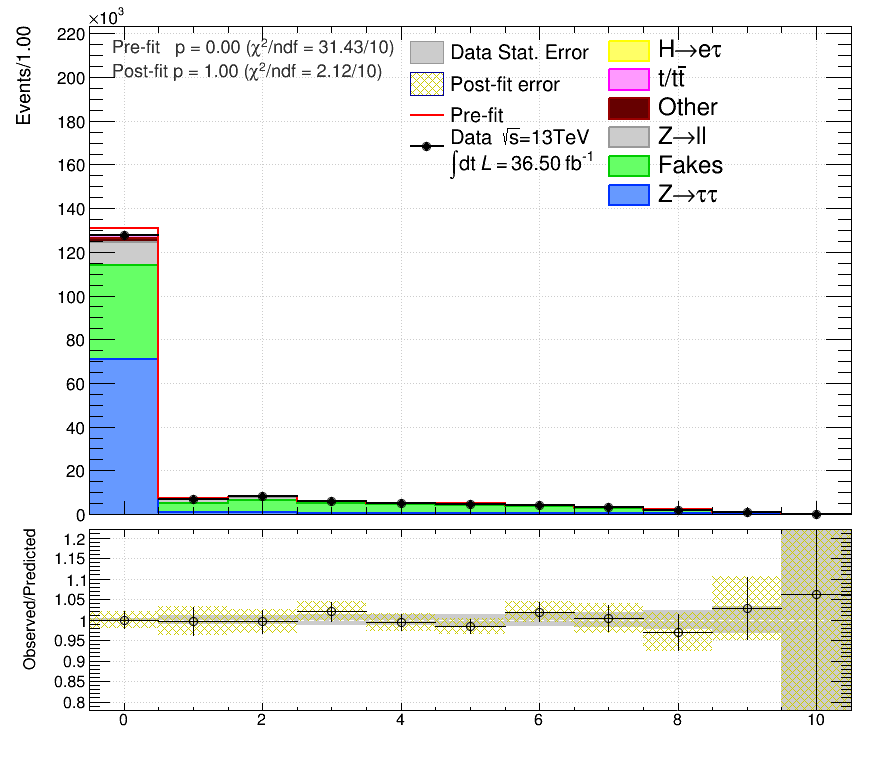
\includegraphics[width=.25\textwidth,height=.30\textheight,type=pdf,ext=.png,read=.png]{/afs/cern.ch/work/a/atpathak/public/FitBox/plots/MMC_etau_inc_regsig_selMVA_liner}
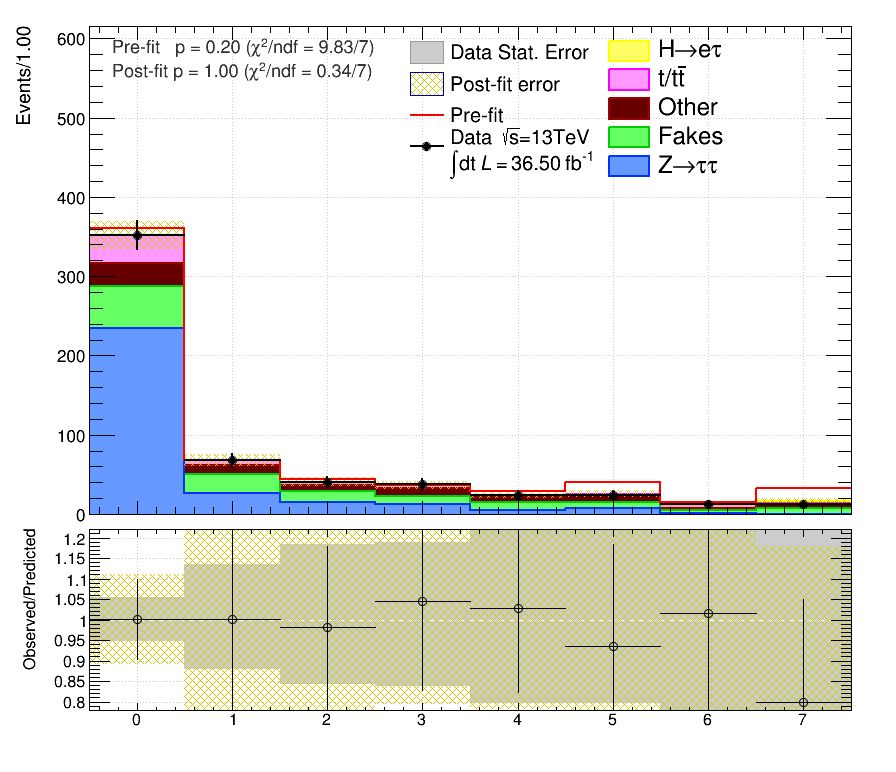
\includegraphics[width=.25\textwidth,height=.30\textheight,type=pdf,ext=.png,read=.png]{/afs/cern.ch/work/a/atpathak/public/FitBox/plots/MMC_etau_vbf_regsig_selMVA_liner}\\
\hspace{0.3in}ll\_inc 
\hspace{0.7in}ll\_vbf
\hspace{0.7in}lh\_inc 
\hspace{0.7in}lh\_VBF
\end{normalsize}
\end{frame}
%-----------------------------------------------
\begin{frame}
\frametitle{Postfit plots for combined ll+lh for MVA in log scale }
\begin{normalsize}
%$\mu\tau_{had}$(top) and \hspace{0.1in}  $e\tau_{had}$(ddZll)(bottom)
\vspace*{0.5cm}
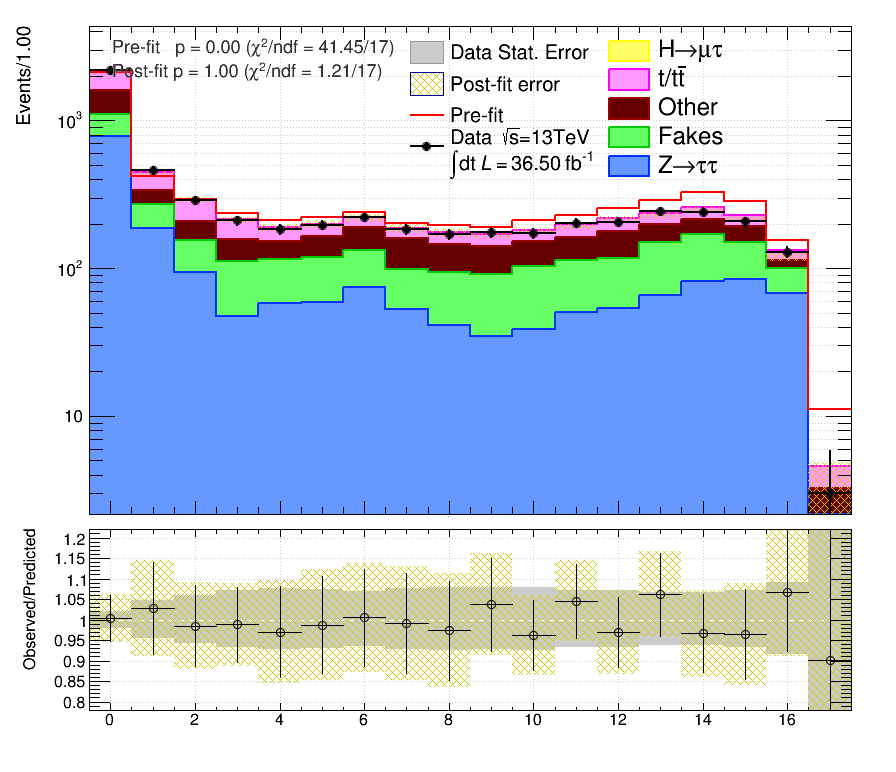
\includegraphics[width=.25\textwidth,height=.30\textheight,type=pdf,ext=.png,read=.png]{/afs/cern.ch/work/a/atpathak/public/FitBox/plots/MMC_me_inc_regsig_selMVA_log}
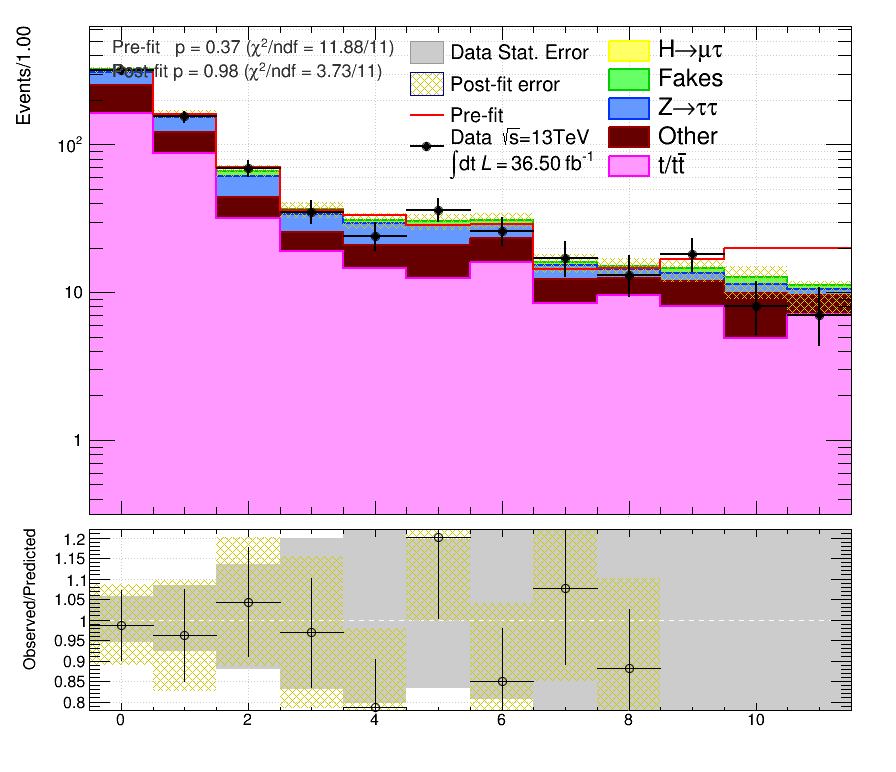
\includegraphics[width=.25\textwidth,height=.30\textheight,type=pdf,ext=.png,read=.png]{/afs/cern.ch/work/a/atpathak/public/FitBox/plots/MMC_me_vbf_regsig_selMVA_log}
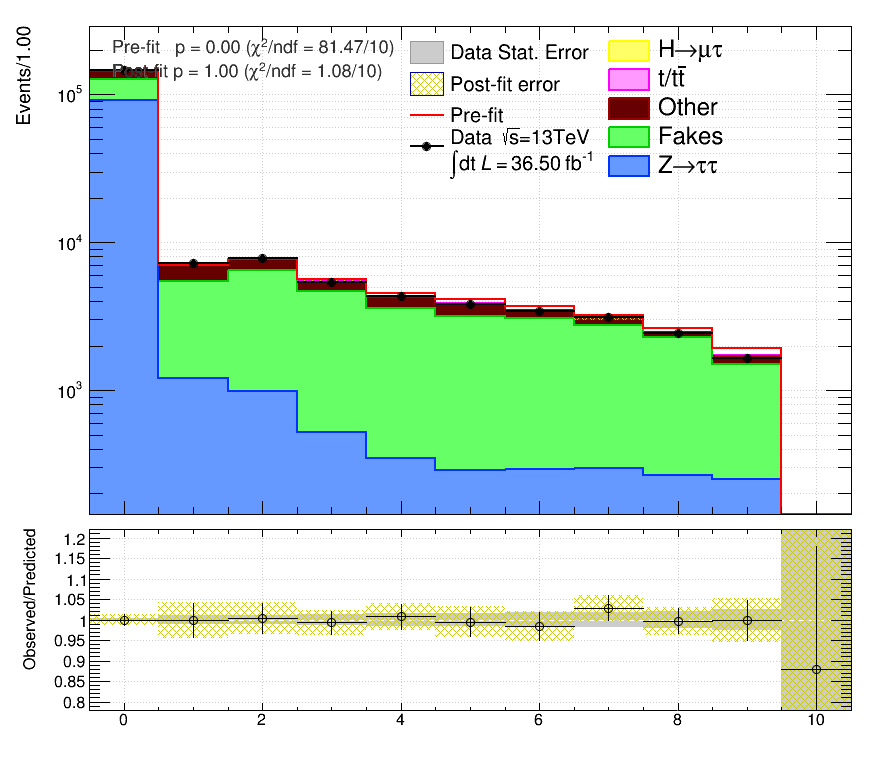
\includegraphics[width=.25\textwidth,height=.30\textheight,type=pdf,ext=.png,read=.png]{/afs/cern.ch/work/a/atpathak/public/FitBox/plots/MMC_mtau_inc_regsig_selMVA_log}
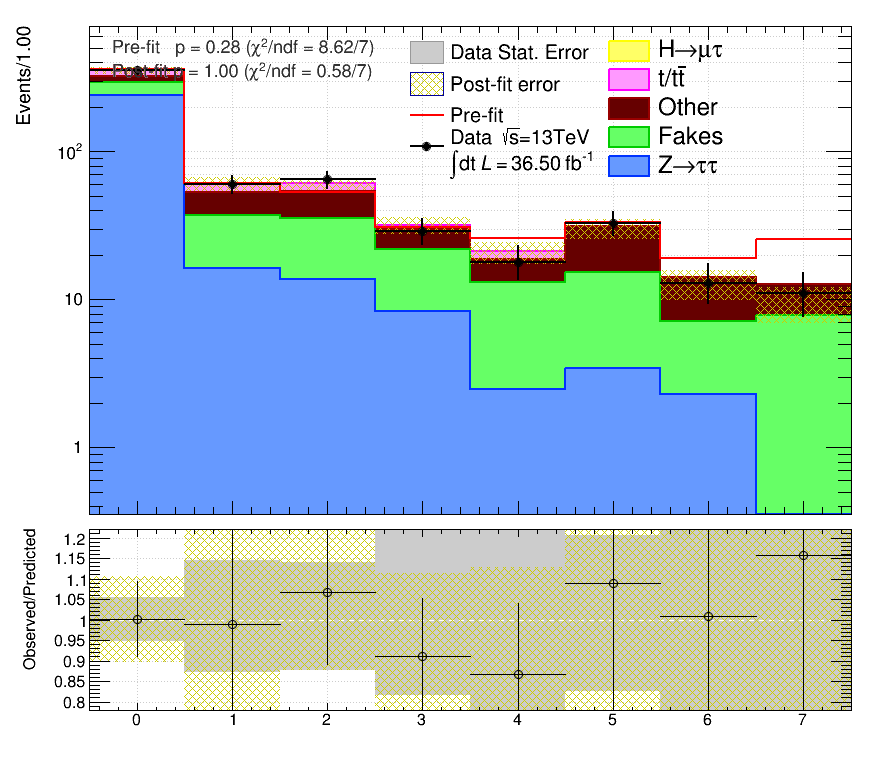
\includegraphics[width=.25\textwidth,height=.30\textheight,type=pdf,ext=.png,read=.png]{/afs/cern.ch/work/a/atpathak/public/FitBox/plots/MMC_mtau_vbf_regsig_selMVA_log}\\
\vspace*{0.5cm}
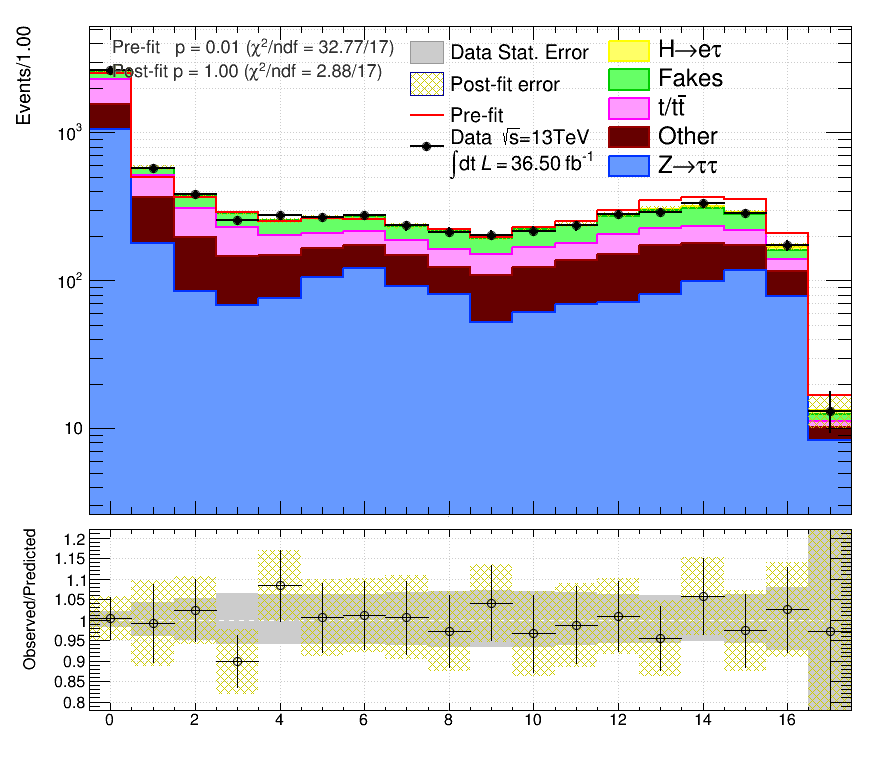
\includegraphics[width=.25\textwidth,height=.30\textheight,type=pdf,ext=.png,read=.png]{/afs/cern.ch/work/a/atpathak/public/FitBox/plots/MMC_em_inc_regsig_selMVA_log}
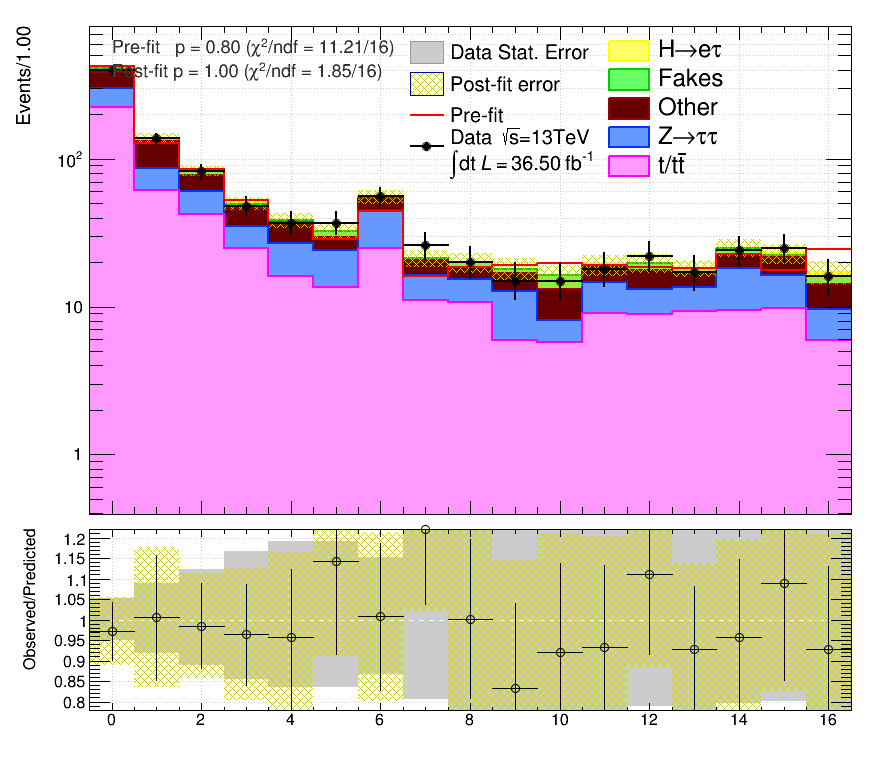
\includegraphics[width=.25\textwidth,height=.30\textheight,type=pdf,ext=.png,read=.png]{/afs/cern.ch/work/a/atpathak/public/FitBox/plots/MMC_em_vbf_regsig_selMVA_log}
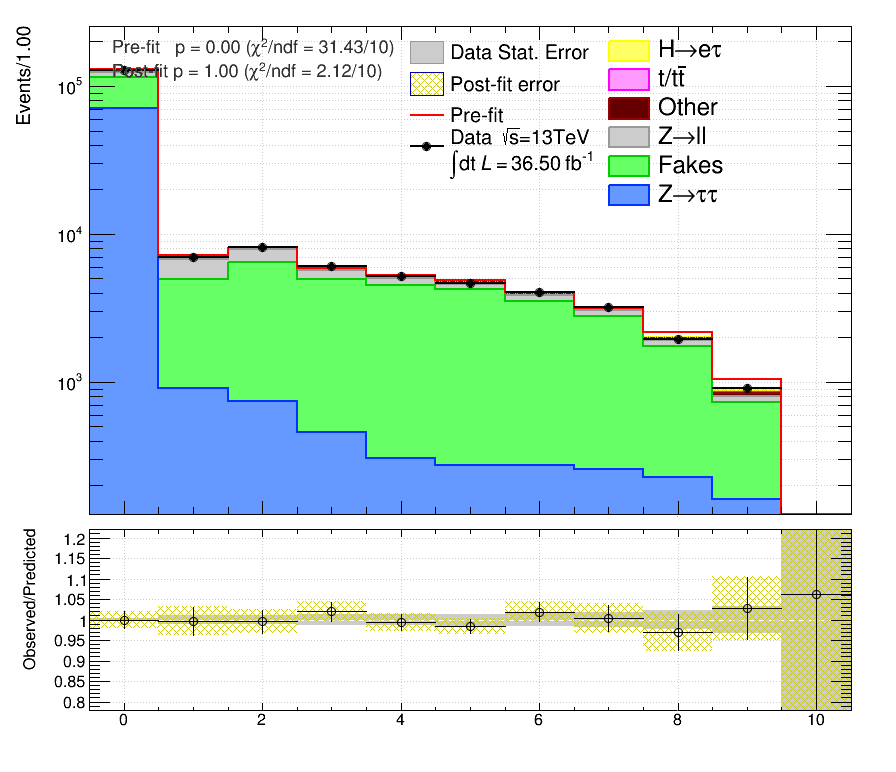
\includegraphics[width=.25\textwidth,height=.30\textheight,type=pdf,ext=.png,read=.png]{/afs/cern.ch/work/a/atpathak/public/FitBox/plots/MMC_etau_inc_regsig_selMVA_log}
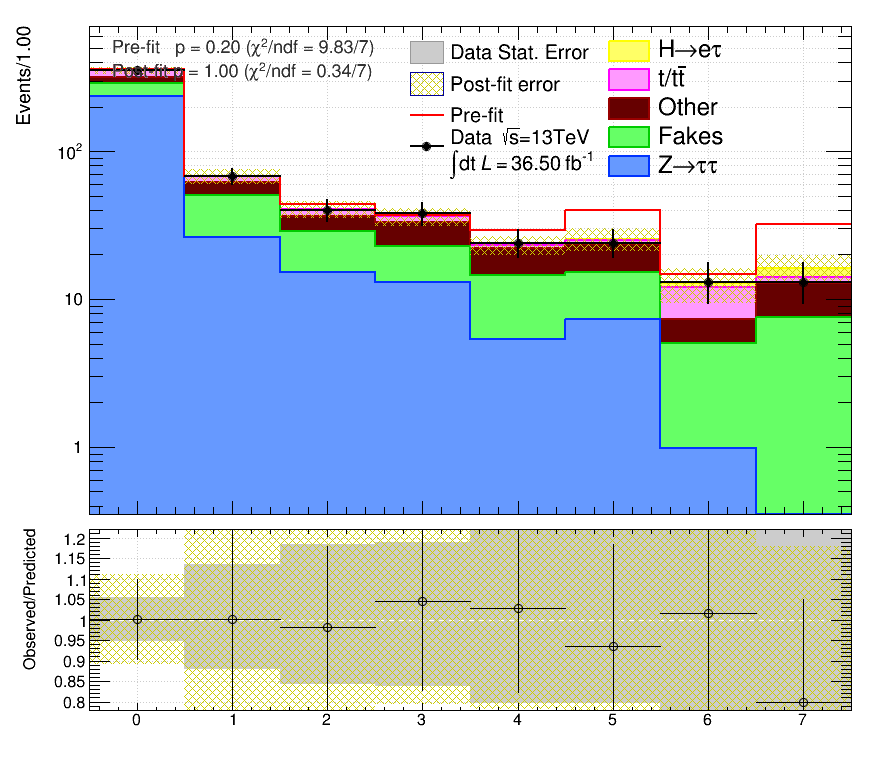
\includegraphics[width=.25\textwidth,height=.30\textheight,type=pdf,ext=.png,read=.png]{/afs/cern.ch/work/a/atpathak/public/FitBox/plots/MMC_etau_vbf_regsig_selMVA_log}\\
\hspace{0.3in}ll\_inc 
\hspace{0.7in}ll\_vbf
\hspace{0.7in}lh\_inc 
\hspace{0.7in}lh\_VBF
\end{normalsize}
\end{frame}
%-----------------------------------------------
\end{document}
%-----------------------------------------------
%-----------------------------------------------
\begin{frame}
\frametitle{Summary Results for CBA for $\mu\tau_{had}$}
\begin{normalsize}
\begin{minipage}{\textwidth}
\begin{minipage}[b]{0.49\textwidth}
\centering
%\vspace*{0.5cm}
%\rule{4cm}{4cm}
\includegraphics[width=.85\textwidth,height=.75\textheight,type=pdf,ext=.pdf,read=.pdf]{/afs/cern.ch/user/a/atpathak/afswork/public/Pixel/LFV_Plots/Plots_Qframework_25Apr2018_Final_note/LFVSummary_result/results_mtau_CBA_updated}\\
\end{minipage}
%\vspace*{5.0cm}
\hfill
\begin{minipage}[b]{0.49\textwidth}
 \centering
 %\vspace*{5.0cm}
 \begin{tabular}{cc}\hline
      Table head & Table head \\ \hline
        Some values & Some values \\
        Some values & Some values \\
        Some values & Some values \\
        Some values & Some values \\
        Some values & Some values \\ 
        Some values & Some values \\ \hline
\end{tabular}
\end{minipage}
\end{minipage}
\end{normalsize}
\end{frame}
%--------------------
\begin{frame}
\frametitle{Significance and Limit for Combined WS}
\vspace*{-0.05cm}
\begin{table}
{\scalebox{.65}{
\begin{tabular}{| l || c | }\hline\hline
channel              &                  Combined(SR'+VBF)                \\\hline
                          &                                                                  \\
$ {\mu\tau}$      &   4.60(0.43 \boldmath${^{+0.17}_{-0.12}}$)  \\ 
                          &                                                                  \\   \hline
                          &                                                                   \\
$ {e\tau}$           &   2.46(0.82 \boldmath${^{+0.32}_{-0.23}}$)    \\ 
                          &                                                                     \\ \hline
                          &                                                                     \\
$ {e\tau}$ddZll   &   4.17(0.48 \boldmath${^{+0.19}_{-0.13}}$)     \\ 
                          &                                                                      \\ \hline
%& & & & \\ \hline
%& & & & \\
%e${\tau}$   & 3.28(0.71 \boldmath${^{+0.28}_{-0.20}}$)  &1.05( 1.90 \boldmath${^{+0.76}_{-0.53}}$ ) & 2.27(0.93 \boldmath${^{+0.36}_{-0.26}}$) & 4.35(0.48 \boldmath${^{+0.19}_{-0.14}}$) \\ 
%& & & & \\ \hline
%& & & & \\
%e${\tau}$ddZll & 4.24(0.49 \boldmath${^{+0.19}_{-0.14}}$)  &2.54( 0.78 \boldmath${^{+0.31}_{-0.22}}$ ) & 2.70(0.78 \boldmath${^{+0.31}_{-0.22}}$) & 5.83(0.35 \boldmath${^{+0.14}_{-0.10}}$) \\ 
%& & & & \\ \hline\hline

\end{tabular}
}}
\end{table}
\end{frame}
%-----------------------------------------------
\begin{frame}
\frametitle{NP Ranking for combined for with ASL and Ztt constrained}
\begin{normalsize}
\hspace{1.2in} $\mu\tau_{had}$
\hspace{1.5in}$e\tau_{had}$ddZll
\vspace*{0.2cm}
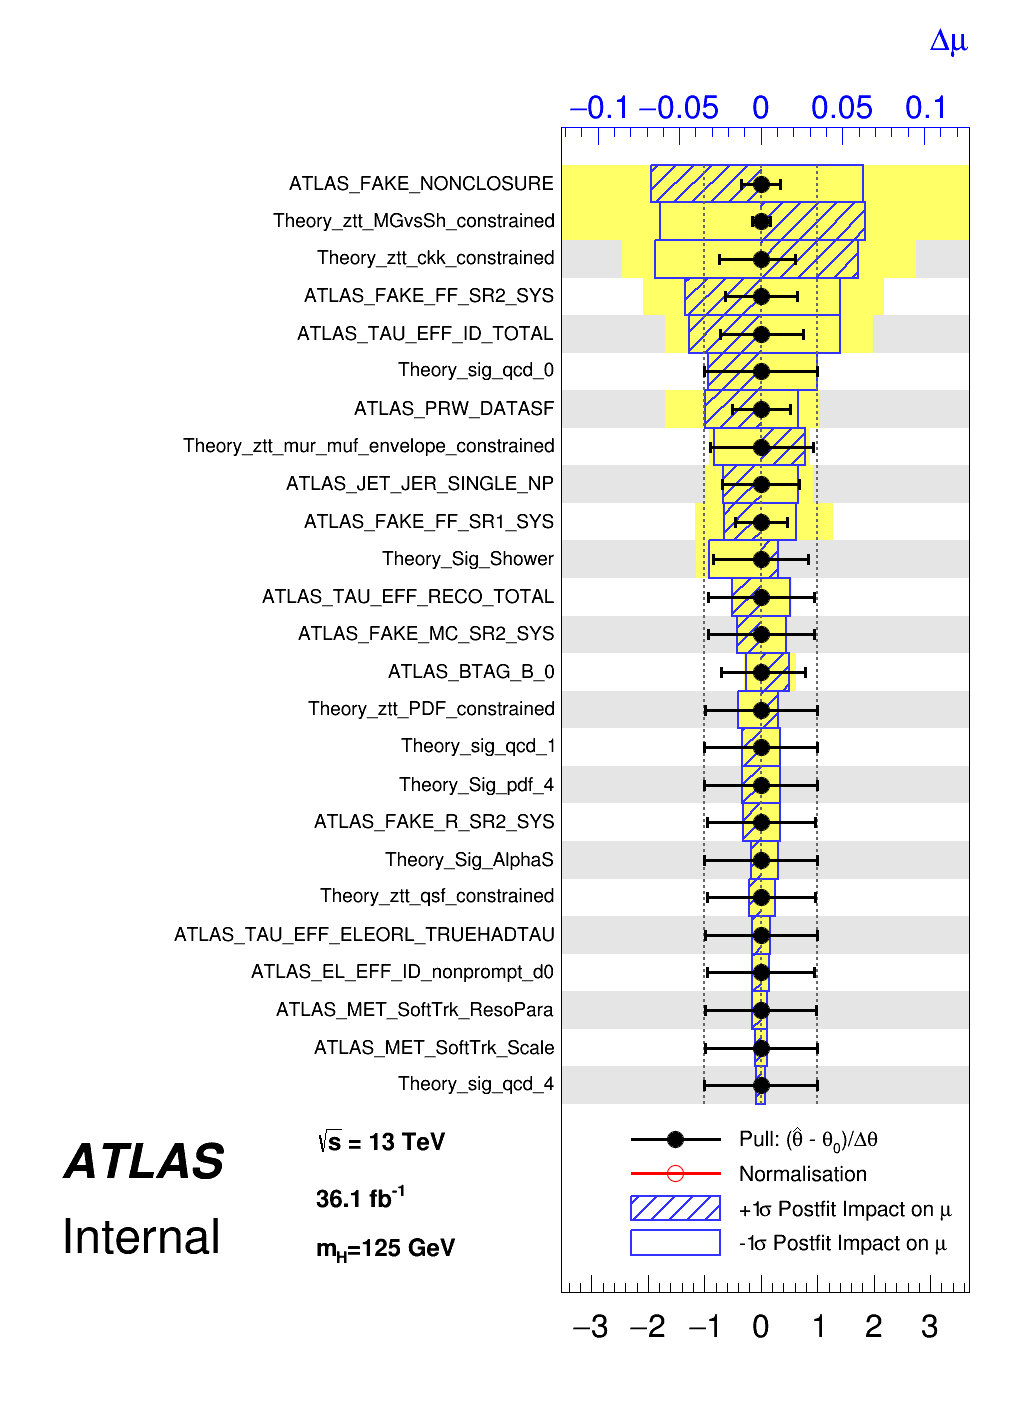
\includegraphics[width=.50\textwidth,height=.70\textheight,type=pdf,ext=.pdf,read=.pdf]{/afs/cern.ch/user/a/atpathak/afswork/public/WSMaker/pdf-files/version/mtau_comb_sr_vbf_ztt_constrained_pulls_125}
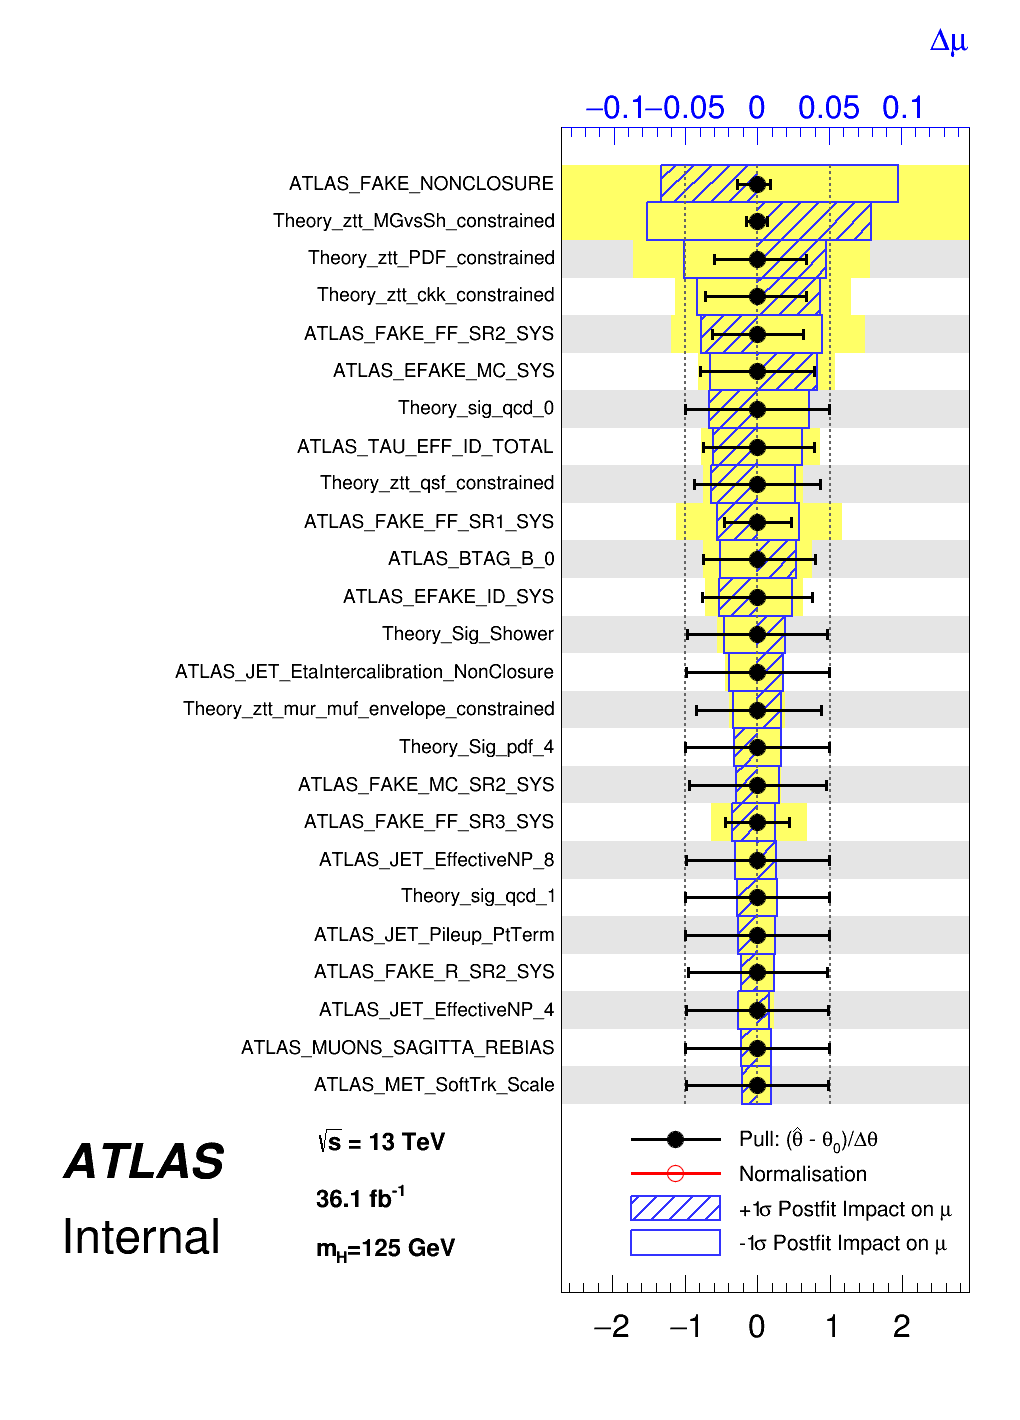
\includegraphics[width=.50\textwidth,height=.70\textheight,type=pdf,ext=.pdf,read=.pdf]{/afs/cern.ch/user/a/atpathak/afswork/public/WSMaker/pdf-files/version/etau_comb_sr_vbf_ddZll_ztt_constrained_pulls_125}
\end{normalsize}
\end{frame}
%-----------------------------------------------
\begin{frame}
\frametitle{Postfit plots for combined SR'+VBF}
\begin{normalsize}
%$\mu\tau_{had}$(top) and \hspace{0.1in}  $e\tau_{had}$(ddZll)(bottom)
\vspace*{0.5cm}
\includegraphics[width=.25\textwidth,height=.30\textheight,type=pdf,ext=.png,read=.png]{/afs/cern.ch/user/a/atpathak/afswork/public/Pixel/LFV_Plots/postfit/mtau_comb_sr_vbf_ztt_constrained/MColl_chanmtau_regsr1vbf_selCBA_signal_}
\includegraphics[width=.25\textwidth,height=.30\textheight,type=pdf,ext=.png,read=.png]{/afs/cern.ch/user/a/atpathak/afswork/public/Pixel/LFV_Plots/postfit/mtau_comb_sr_vbf_ztt_constrained/MColl_chanmtau_regsr2vbf_selCBA_signal_}
\includegraphics[width=.25\textwidth,height=.30\textheight,type=pdf,ext=.png,read=.png]{/afs/cern.ch/user/a/atpathak/afswork/public/Pixel/LFV_Plots/postfit/mtau_comb_sr_vbf_ztt_constrained/MColl_chanmtau_regsr3vbf_selCBA_signal_}
\includegraphics[width=.25\textwidth,height=.30\textheight,type=pdf,ext=.png,read=.png]{/afs/cern.ch/user/a/atpathak/afswork/public/Pixel/LFV_Plots/postfit/mtau_comb_sr_vbf_ztt_constrained/MColl_chanmtau_regvbf_selCBA_signal_}\\
\vspace*{0.5cm}
\includegraphics[width=.25\textwidth,height=.30\textheight,type=pdf,ext=.png,read=.png]{/afs/cern.ch/user/a/atpathak/afswork/public/Pixel/LFV_Plots/postfit/etau_comb_sr_vbf_ddZll_ztt_constrained/MColl_chanetau_regsr1vbf_selCBA_signal_}
\includegraphics[width=.25\textwidth,height=.30\textheight,type=pdf,ext=.png,read=.png]{/afs/cern.ch/user/a/atpathak/afswork/public/Pixel/LFV_Plots/postfit/etau_comb_sr_vbf_ddZll_ztt_constrained/MColl_chanetau_regsr2vbf_selCBA_signal_}
\includegraphics[width=.25\textwidth,height=.30\textheight,type=pdf,ext=.png,read=.png]{/afs/cern.ch/user/a/atpathak/afswork/public/Pixel/LFV_Plots/postfit/etau_comb_sr_vbf_ddZll_ztt_constrained/MColl_chanetau_regsr3vbf_selCBA_signal_}
\includegraphics[width=.25\textwidth,height=.30\textheight,type=pdf,ext=.png,read=.png]{/afs/cern.ch/user/a/atpathak/afswork/public/Pixel/LFV_Plots/postfit/etau_comb_sr_vbf_ddZll_ztt_constrained/MColl_chanetau_regvbf_selCBA_signal_}\\
\hspace{0.5in}SR1 
\hspace{0.75in}SR2
\hspace{0.75in}SR3
\hspace{0.75in}VBF
\end{normalsize}
\end{frame}
%-----------------------------------------------
\end{document}
%-----------------------------------------------
\begin{frame}
\frametitle{Significance for Combined WS}
\vspace*{-0.05cm}
\begin{table}
{\scalebox{.65}{
\begin{tabular}{| l | c | c | c |c | c | c | c || c | c |}\hline\hline
Channel      &               &              \multicolumn {2}{c|} {SR1}                        &                  \multicolumn {2}{c|} {SR2}                     &              \multicolumn {2}{c||} {SR3}           & \multicolumn {2}{c|} {Combined}  \\  \cline{3-10}
                  &                &         Default      &ll                                               &Default&ll                                                                &Default&ll                                                  &Default&ll                                       \\
                  &                &            bin        &bin                                             &bin&bin                                                                    &bin&bin                                                      &bin&bin                                          \\\hline
$ {\mu\tau}$ &no ASL    &          3.04         &2.41                                           &1.60 &0.92                                                               &1.40 &1.46                                                 &4.26 &3.42 \\
% & & & & & & & & & \\\cline{2-10}
%& & & & & & & & & \\
                 & With ASL& 2.99& 2.41                                                        & 1.63&0.96                                                                   &1.40 & 1.46                                               &4.26 & 3.43\\
\hline
$ {e\tau}$ &no ASL    & 1.77 &1.62                                                        &0.72 &0.49                                                                    &1.21 &0.72                                                &2.49 &2.38 \\
% & & & & & & & & & \\\cline{2-10}
%& & & & & & & & & \\
                 & With ASL& 1.73& 1.61                                                      & 0.72&0.50                                                                  &1.21 & 0.72                                               &2.42 & 2.32\\\hline

%&  & 2.91(0.68 \boldmath${^{+0.27}_{-0.19}}$) & 1.58(1.27 \boldmath${^{+0.50}_{-0.36}}$) & 5.63(0.35 \boldmath${^{+0.14}_{-0.10}}$) \\ 
%& & & & \\ \hline
%& & & & \\
%e${\tau}$   & 3.28(0.71 \boldmath${^{+0.28}_{-0.20}}$)  &1.05( 1.90 \boldmath${^{+0.76}_{-0.53}}$ ) & 2.27(0.93 \boldmath${^{+0.36}_{-0.26}}$) & 4.35(0.48 \boldmath${^{+0.19}_{-0.14}}$) \\ 
%& & & & \\ \hline
%& & & & \\
%e${\tau}$ddZll & 4.24(0.49 \boldmath${^{+0.19}_{-0.14}}$)  &2.54( 0.78 \boldmath${^{+0.31}_{-0.22}}$ ) & 2.70(0.78 \boldmath${^{+0.31}_{-0.22}}$) & 5.83(0.35 \boldmath${^{+0.14}_{-0.10}}$) \\ 
%& & & & \\ \hline\hline

\end{tabular}
}}
\end{table}
\begin{table}
{\scalebox{.65}{
\begin{tabular}{| l | c | c | c |c | c | c | c | c | c || c | c |}\hline\hline

Channel      &               &\multicolumn {2}{c|} {SR1'}&\multicolumn {2}{c|} {SR2'} &\multicolumn {2}{c|} {SR3'} &\multicolumn {2}{c||} {VBF} & \multicolumn {2}{c|} {Combined}  \\  \cline{3-12}
                  &                &      Default     &   ll            &Default&ll                          &Default&ll                          &Default&ll                           &Default&ll                                     \\
                  &                &         bin        &  bin            &bin&bin                             &bin&bin                             &bin&bin                              &bin&bin                                        \\\hline
$ {\mu\tau}$ &no ASL &  3.13            & 2.31             & 1.54& 0.90                       & 1.31& 1.44                       &1.66 & 1.41                        & 4.60   & 3.63                               \\
                     &With ASL& 3.14            &2.31              &1.57 &0.93                        &1.34 & 1.45                       &1.66 & 1.40                        &4.83    & 3.65                               \\
\hline
$ {e\tau}$     &no ASL &  1.68            & 1.55             & 0.69& 0.47                       & 1.17& 0.71                       &0.81 & 0.79                       & 2.53   & 2.42                               \\
                     &With ASL& 1.64            &1.54              &0.69&0.49                       &1.17 & 0.73                       &0.79 & 0.78                       &2.47    & 2.35                               \\\hline
%$ {\mu\tau}$ & 4.41(0.44 \boldmath${^{+0.17}_{-0.12}}$) & 2.84(0.70 \boldmath${^{+0.27}_{-0.20}}$) & 1.45(1.36 \boldmath${^{+0.53}_{-0.38}}$) & 2.29(0.88 \boldmath${^{+0.35}_{-0.25}}$) & 6.14(0.32 \boldmath${^{+0.12}_{-0.09}}$) \\ 
%& & & & & \\ \hline
%& & & & & \\
%e${\tau}$   & 3.11(0.71 \boldmath${^{+0.28}_{-0.20}}$)  & 1.00( 1.99 \boldmath${^{+0.80}_{-0.56}}$ ) & 2.21(0.95 \boldmath${^{+0.37}_{-0.26}}$) & 1.05(1.80 \boldmath${^{+0.66}_{-0.51}}$) & 4.38(0.47 \boldmath${^{+0.18}_{-0.13}}$) \\ 
%& & & & & \\ \hline
%& & & & & \\
%e${\tau}$ddZll & 4.02(0.51 \boldmath${^{+0.20}_{-0.14}}$)  & 2.42( 0.82 \boldmath${^{+0.32}_{-0.23}}$ ) & 2.59(0.81 \boldmath${^{+0.32}_{-0.23}}$) & 1.46(1.33 \boldmath${^{+0.52}_{-0.37}}$) & 5.77(0.35 \boldmath${^{+0.14}_{-0.10}}$) \\ 
%& & & & & \\ \hline\hline
\end{tabular}
}}
\end{table}
\end{frame}
%-----------------------------------------------
\begin{frame}
\frametitle{Limit for Combined WS}
\vspace*{-0.05cm}
\begin{table}
{\scalebox{.55}{
\begin{tabular}{| l | c | c | c |c | c | c | c || c | c |}\hline\hline
Channel      &               &              \multicolumn {2}{c|} {SR1}                                                     &                  \multicolumn {2}{c|} {SR2}                     &              \multicolumn {2}{c||} {SR3}                                                                                                     & \multicolumn {2}{c|} {Combined}  \\  \cline{3-10}
                  &                &         Default  &   ll                                                                                &Default&ll                                                                &Default&ll                                                                                                                                          &       Default  &            ll                                       \\
                  &                &            bin    &bin                                                                                &bin&bin                                                                    &bin&bin                                                                                                                                              &bin&bin                                          \\\hline

$ {\mu\tau}$ &no ASL &0.66 \boldmath${^{+0.26}_{-0.18}}$&0.82 \boldmath${^{+0.32}_{-0.23}}$  &1.24\boldmath${^{+0.48}_{-0.34}}$ & 2.10 \boldmath${^{+ 0.76}_{-0.61}}$&1.41\boldmath${^{+0.55}_{-0.39}}$ &1.36\boldmath${^{+0.53}_{-0.38}}$                                                 &0.47 \boldmath${^{+0.18}_{-0.13}}$&0.59 \boldmath${^{+0.23}_{-0.16}}$ \\
& & & & & & & & & \\
%& & & & & & & & & \\
                 & With ASL& 0.68 \boldmath${^{+0.26}_{-0.19}}$& 0.82 \boldmath${^{+0.32}_{-0.23}}$ & 1.21 \boldmath${^{+ 0.47}_{-0.34}}$& 2.09 \boldmath${^{+ 0.82}_{-0.59}}$&1.41\boldmath${^{+0.55}_{-0.39}}$ & 1.36\boldmath${^{+0.53}_{-0.38}}$                                            &0.47 \boldmath${^{+0.18}_{-0.13}}$ & 0.58 \boldmath${^{+0.23}_{-0.16}}$\\
\hline
$ {e\tau}$ &no ASL &1.21 \boldmath${^{+0.44}_{-0.31}}$&1.23 \boldmath${^{+0.48}_{-0.34}}$  &2.72\boldmath${^{+1.03}_{-0.76}}$ & 3.94 \boldmath${^{+ 1.31}_{-1.1}}$&1.63\boldmath${^{+0.65}_{-0.45}}$ &2.77\boldmath${^{+1.11}_{-0.77}}$                                                 &0.81 \boldmath${^{+0.32}_{-0.23}}$&0.85 \boldmath${^{+0.33}_{-0.24}}$ \\
& & & & & & & & & \\
%& & & & & & & & & \\
                 & With ASL& 1.21 \boldmath${^{+0.48}_{-0.33}}$& 1.30 \boldmath${^{+0.50}_{-0.36}}$ & 2.68 \boldmath${^{+ 1.03}_{-0.75}}$& 3.90 \boldmath${^{+ 1.42}_{-1.09}}$&1.69\boldmath${^{+0.69}_{-0.47}}$ &2.95\boldmath${^{+1.25}_{-0.82}}$                                            &0.84 \boldmath${^{+0.33}_{-0.23}}$ & 0.90 \boldmath${^{+0.35}_{-0.25}}$\\\hline

\end{tabular}
}}
\end{table}
\begin{table}
{\scalebox{.47}{
\begin{tabular}{| l | c | c | c |c | c | c | c | c | c || c | c |}\hline\hline
Channel      &               &              \multicolumn {2}{c|} {SR1'}                                                     &                  \multicolumn {2}{c|} {SR2'}                     &              \multicolumn {2}{c|} {SR3'}                                                                                                     &  \multicolumn {2}{c||} {VBF}             & \multicolumn {2}{c|} {Combined}  \\  \cline{3-12}
                  &                &         Default  &   ll                                                                                &Default&ll                                                                &Default&ll                                                                                                                                          &       Default  &            ll                 &       Default  &            ll                                       \\
                  &                &            bin    &bin                                                                                &bin&bin                                                                    &bin&bin                                                                                                                                              &bin&bin                                        &bin&bin                                          \\\hline

$ {\mu\tau}$ &no ASL &0.64 \boldmath${^{+0.25}_{-0.18}}$&0.86 \boldmath${^{+0.33}_{-0.24}}$  &1.29\boldmath${^{+0.50}_{-0.36}}$ & 2.14 \boldmath${^{+ 0.79}_{-0.60}}$ &1.49\boldmath${^{+0.58}_{-0.41}}$ &1.37\boldmath${^{+0.53}_{-0.38}}$                                                 &1.22 \boldmath${^{+0.48}_{-0.34}}$ & 1.44 \boldmath${^{+0.56}_{-0.40}}$ & 0.43 \boldmath${^{+0.17}_{-0.12}}$&0.55 \boldmath${^{+0.21}_{-0.15}}$ \\
& & & & & & & & & & & \\
%& & & & & & & & & \\
                 & With ASL& 0.64 \boldmath${^{+0.25}_{-0.17}}$& 0.86 \boldmath${^{+0.33}_{-0.24}}$ & 1.26 \boldmath${^{+ 0.49}_{-0.35}}$&2.14 \boldmath${^{+ 0.85}_{-0.60}}$ &1.48\boldmath${^{+0.58}_{-0.41}}$ & 1.37\boldmath${^{+0.53}_{-0.38}}$                                            &1.22 \boldmath${^{+0.48}_{-0.34}}$ & 1.44 \boldmath${^{+0.56}_{-0.40}}$ & 0.41 \boldmath${^{+0.16}_{-0.11}}$ & 0.54 \boldmath${^{+0.21}_{-0.15}}$\\
\hline
$ {e\tau}$ &no ASL &1.18 \boldmath${^{+0.46}_{-0.33}}$&1.28 \boldmath${^{+0.50}_{-0.35}}$  &2.83\boldmath${^{+1.07}_{-0.79}}$ & 4.09 \boldmath${^{+ 1.36}_{-1.14}}$ &1.69\boldmath${^{+0.66}_{-0.47}}$ &2.78\boldmath${^{+1.12}_{-0.78}}$                                                 &2.22 \boldmath${^{+0.8}_{-0.62}}$ & 2.38 \boldmath${^{+0.88}_{-0.67}}$ & 0.79 \boldmath${^{+0.31}_{-0.22}}$&0.83 \boldmath${^{+0.33}_{-0.23}}$ \\
& & & & & & & & & & & \\
%& & & & & & & & & \\
                 & With ASL& 1.26 \boldmath${^{+0.49}_{-0.35}}$& 1.36 \boldmath${^{+0.53}_{-0.38}}$ & 2.80 \boldmath${^{+ 1.07}_{-0.78}}$&4.07 \boldmath${^{+ 1.48}_{-1.14}}$ &1.75\boldmath${^{+0.72}_{-0.49}}$ & 2.99\boldmath${^{+1.29}_{-0.83}}$                                            &2.29 \boldmath${^{+0.82}_{-0.64}}$ & 2.43 \boldmath${^{+0.93}_{-0.68}}$ & 0.82 \boldmath${^{+0.32}_{-0.23}}$ & 0.88 \boldmath${^{+0.34}_{-0.25}}$\\\hline
\end{tabular}
}}
\end{table}
\end{frame}
%-----------------------------------------------
\begin{frame}
\frametitle{NP Ranking for combined $\mu\tau_{had}$ for with ASL}
\begin{normalsize}
\hspace{1.2in}Default bin 
\hspace{1.5in}Leplep bin
\vspace*{0.2cm}
\includegraphics[width=.50\textwidth,height=.70\textheight,type=pdf,ext=.pdf,read=.pdf]{/afs/cern.ch/user/a/atpathak/afswork/public/WSMaker/pdf-files/version/mtau_comb_sr_vbf_new_pulls_125}
\includegraphics[width=.50\textwidth,height=.70\textheight,type=pdf,ext=.pdf,read=.pdf]{/afs/cern.ch/user/a/atpathak/afswork/public/WSMaker/pdf-files/version/mtau_comb_sr_vbf_llbin_pulls_125}
\end{normalsize}
\end{frame}
%-----------------------------------------------
\begin{frame}
\frametitle{NP Ranking for combined $\mu\tau_{had}$ for no ASL}
\begin{normalsize}
\hspace{1.2in}Default bin 
\hspace{1.5in}Leplep bin
\vspace*{0.2cm}
\includegraphics[width=.50\textwidth,height=.70\textheight,type=pdf,ext=.pdf,read=.pdf]{/afs/cern.ch/user/a/atpathak/afswork/public/WSMaker/pdf-files/version/mtau_comb_sr_vbf_noAgg_pulls_125}
\includegraphics[width=.50\textwidth,height=.70\textheight,type=pdf,ext=.pdf,read=.pdf]{/afs/cern.ch/user/a/atpathak/afswork/public/WSMaker/pdf-files/version/mtau_comb_sr_vbf_llbin_noAgg_pulls_125}
\end{normalsize}
\end{frame}
%-----------------------------------------------
\begin{frame}
\frametitle{NP Ranking for combined $e\tau_{had}$ for with ASL}
\begin{normalsize}
\hspace{1.2in}Default bin 
\hspace{1.5in}Leplep bin
\vspace*{0.2cm}
\includegraphics[width=.50\textwidth,height=.70\textheight,type=pdf,ext=.pdf,read=.pdf]{/afs/cern.ch/user/a/atpathak/afswork/public/WSMaker/pdf-files/version/etau_comb_sr_vbf_pulls_125}
\includegraphics[width=.50\textwidth,height=.70\textheight,type=pdf,ext=.pdf,read=.pdf]{/afs/cern.ch/user/a/atpathak/afswork/public/WSMaker/pdf-files/version/etau_comb_sr_vbf_llbin_pulls_125}
\end{normalsize}
\end{frame}
%-----------------------------------------------
\begin{frame}
\frametitle{NP Ranking for combined $e\tau_{had}$ for no ASL}
\begin{normalsize}
\hspace{1.2in}Default bin 
\hspace{1.5in}Leplep bin
\vspace*{0.2cm}
\includegraphics[width=.50\textwidth,height=.70\textheight,type=pdf,ext=.pdf,read=.pdf]{/afs/cern.ch/user/a/atpathak/afswork/public/WSMaker/pdf-files/version/etau_comb_sr_vbf_noAgg_pulls_125}
\includegraphics[width=.50\textwidth,height=.70\textheight,type=pdf,ext=.pdf,read=.pdf]{/afs/cern.ch/user/a/atpathak/afswork/public/WSMaker/pdf-files/version/etau_comb_sr_vbf_llbin_noAgg_pulls_125}
\end{normalsize}
\end{frame}
%-----------------------------------------------
\end{document}
%-----------------------------------------------
\begin{frame}
\frametitle{Distributions of $\mu\tau_{had}$ events in the SR1 region.}
\begin{normalsize}
\vspace*{0.2cm}
\includegraphics[width=.30\textwidth,height=.30\textheight,type=pdf,ext=.pdf,read=.pdf]{/afs/cern.ch/user/a/atpathak/afswork/public/Pixel/LFV_Plots/Plots_Qframework_25Apr2018_Final_note/plots_mcZll/mtau-CutTauMTSR1-leptonPt-lin}
\includegraphics[width=.30\textwidth,height=.30\textheight,type=pdf,ext=.pdf,read=.pdf]{/afs/cern.ch/user/a/atpathak/afswork/public/Pixel/LFV_Plots/Plots_Qframework_25Apr2018_Final_note/plots_mcZll/mtau-CutTauMTSR1-tauPt-lin}
\includegraphics[width=.30\textwidth,height=.30\textheight,type=pdf,ext=.pdf,read=.pdf]{/afs/cern.ch/user/a/atpathak/afswork/public/Pixel/LFV_Plots/Plots_Qframework_25Apr2018_Final_note/plots_mcZll/mtau-CutTauMTSR1-dEtaTauLep-lin}\\
\includegraphics[width=.30\textwidth,height=.30\textheight,type=pdf,ext=.pdf,read=.pdf]{/afs/cern.ch/user/a/atpathak/afswork/public/Pixel/LFV_Plots/Plots_Qframework_25Apr2018_Final_note/plots_mcZll/mtau-CutTauMTSR1-transverseMassLepMET-lin}
\includegraphics[width=.30\textwidth,height=.30\textheight,type=pdf,ext=.pdf,read=.pdf]{/afs/cern.ch/user/a/atpathak/afswork/public/Pixel/LFV_Plots/Plots_Qframework_25Apr2018_Final_note/plots_mcZll/mtau-CutTauMTSR1-transverseMassTauMET-lin}
\includegraphics[width=.30\textwidth,height=.30\textheight,type=pdf,ext=.pdf,read=.pdf]{/afs/cern.ch/user/a/atpathak/afswork/public/Pixel/LFV_Plots/Plots_Qframework_25Apr2018_Final_note/plots_mcZll/mtau-CutTauMTSR1-met-lin}\\
\includegraphics[width=.30\textwidth,height=.30\textheight,type=pdf,ext=.pdf,read=.pdf]{/afs/cern.ch/user/a/atpathak/afswork/public/Pixel/LFV_Plots/Plots_Qframework_25Apr2018_Final_note/plots_mcZll/mtau-CutTauMTSR1-visibleMass-lin}
\includegraphics[width=.30\textwidth,height=.30\textheight,type=pdf,ext=.pdf,read=.pdf]{/afs/cern.ch/user/a/atpathak/afswork/public/Pixel/LFV_Plots/Plots_Qframework_25Apr2018_Final_note/plots_mcZll/mtau-CutTauMTSR1-collMassBL-lin}
\includegraphics[width=.30\textwidth,height=.30\textheight,type=pdf,ext=.pdf,read=.pdf]{/afs/cern.ch/user/a/atpathak/afswork/public/Pixel/LFV_Plots/Plots_Qframework_25Apr2018_Final_note/plots_mcZll/mtau-CutTauMTSR1-MMCBL-lin}
\end{normalsize}
\end{frame}
%-----------------------------------------------
\begin{frame}
\frametitle{Distributions of $\mu\tau_{had}$ events in the SR2 region(mvis cut).}
\begin{normalsize}
\vspace*{0.2cm}
\includegraphics[width=.30\textwidth,height=.30\textheight,type=pdf,ext=.pdf,read=.pdf]{/afs/cern.ch/user/a/atpathak/afswork/public/Pixel/LFV_Plots/Plots_Qframework_25Apr2018_Final_note/plots_mcZll/mtau-CutTauMTSR2_Mvis-leptonPt-lin}
\includegraphics[width=.30\textwidth,height=.30\textheight,type=pdf,ext=.pdf,read=.pdf]{/afs/cern.ch/user/a/atpathak/afswork/public/Pixel/LFV_Plots/Plots_Qframework_25Apr2018_Final_note/plots_mcZll/mtau-CutTauMTSR2_Mvis-tauPt-lin}
\includegraphics[width=.30\textwidth,height=.30\textheight,type=pdf,ext=.pdf,read=.pdf]{/afs/cern.ch/user/a/atpathak/afswork/public/Pixel/LFV_Plots/Plots_Qframework_25Apr2018_Final_note/plots_mcZll/mtau-CutTauMTSR2_Mvis-dEtaTauLep-lin}\\
\includegraphics[width=.30\textwidth,height=.30\textheight,type=pdf,ext=.pdf,read=.pdf]{/afs/cern.ch/user/a/atpathak/afswork/public/Pixel/LFV_Plots/Plots_Qframework_25Apr2018_Final_note/plots_mcZll/mtau-CutTauMTSR2_Mvis-transverseMassLepMET-lin}
\includegraphics[width=.30\textwidth,height=.30\textheight,type=pdf,ext=.pdf,read=.pdf]{/afs/cern.ch/user/a/atpathak/afswork/public/Pixel/LFV_Plots/Plots_Qframework_25Apr2018_Final_note/plots_mcZll/mtau-CutTauMTSR2_Mvis-transverseMassTauMET-lin}
\includegraphics[width=.30\textwidth,height=.30\textheight,type=pdf,ext=.pdf,read=.pdf]{/afs/cern.ch/user/a/atpathak/afswork/public/Pixel/LFV_Plots/Plots_Qframework_25Apr2018_Final_note/plots_mcZll/mtau-CutTauMTSR2_Mvis-met-lin}\\
\includegraphics[width=.30\textwidth,height=.30\textheight,type=pdf,ext=.pdf,read=.pdf]{/afs/cern.ch/user/a/atpathak/afswork/public/Pixel/LFV_Plots/Plots_Qframework_25Apr2018_Final_note/plots_mcZll/mtau-CutTauMTSR2_Mvis-visibleMass-lin}
\includegraphics[width=.30\textwidth,height=.30\textheight,type=pdf,ext=.pdf,read=.pdf]{/afs/cern.ch/user/a/atpathak/afswork/public/Pixel/LFV_Plots/Plots_Qframework_25Apr2018_Final_note/plots_mcZll/mtau-CutTauMTSR2_Mvis-collMassBL-lin}
\includegraphics[width=.30\textwidth,height=.30\textheight,type=pdf,ext=.pdf,read=.pdf]{/afs/cern.ch/user/a/atpathak/afswork/public/Pixel/LFV_Plots/Plots_Qframework_25Apr2018_Final_note/plots_mcZll/mtau-CutTauMTSR2_Mvis-MMCBL-lin}
\end{normalsize}
\end{frame}
%-----------------------------------------------
\begin{frame}
\frametitle{Distributions of $\mu\tau_{had}$ events in the SR3 region.}
\begin{normalsize}
\vspace*{0.2cm}
\includegraphics[width=.30\textwidth,height=.30\textheight,type=pdf,ext=.pdf,read=.pdf]{/afs/cern.ch/user/a/atpathak/afswork/public/Pixel/LFV_Plots/Plots_Qframework_25Apr2018_Final_note/plots_mcZll/mtau-CutTauPtSR3-leptonPt-lin}
\includegraphics[width=.30\textwidth,height=.30\textheight,type=pdf,ext=.pdf,read=.pdf]{/afs/cern.ch/user/a/atpathak/afswork/public/Pixel/LFV_Plots/Plots_Qframework_25Apr2018_Final_note/plots_mcZll/mtau-CutTauPtSR3-tauPt-lin}
\includegraphics[width=.30\textwidth,height=.30\textheight,type=pdf,ext=.pdf,read=.pdf]{/afs/cern.ch/user/a/atpathak/afswork/public/Pixel/LFV_Plots/Plots_Qframework_25Apr2018_Final_note/plots_mcZll/mtau-CutTauPtSR3-dEtaTauLep-lin}\\
\includegraphics[width=.30\textwidth,height=.30\textheight,type=pdf,ext=.pdf,read=.pdf]{/afs/cern.ch/user/a/atpathak/afswork/public/Pixel/LFV_Plots/Plots_Qframework_25Apr2018_Final_note/plots_mcZll/mtau-CutTauPtSR3-transverseMassLepMET-lin}
\includegraphics[width=.30\textwidth,height=.30\textheight,type=pdf,ext=.pdf,read=.pdf]{/afs/cern.ch/user/a/atpathak/afswork/public/Pixel/LFV_Plots/Plots_Qframework_25Apr2018_Final_note/plots_mcZll/mtau-CutTauPtSR3-transverseMassTauMET-lin}
\includegraphics[width=.30\textwidth,height=.30\textheight,type=pdf,ext=.pdf,read=.pdf]{/afs/cern.ch/user/a/atpathak/afswork/public/Pixel/LFV_Plots/Plots_Qframework_25Apr2018_Final_note/plots_mcZll/mtau-CutTauPtSR3-met-lin}\\
\includegraphics[width=.30\textwidth,height=.30\textheight,type=pdf,ext=.pdf,read=.pdf]{/afs/cern.ch/user/a/atpathak/afswork/public/Pixel/LFV_Plots/Plots_Qframework_25Apr2018_Final_note/plots_mcZll/mtau-CutTauPtSR3-visibleMass-lin}
\includegraphics[width=.30\textwidth,height=.30\textheight,type=pdf,ext=.pdf,read=.pdf]{/afs/cern.ch/user/a/atpathak/afswork/public/Pixel/LFV_Plots/Plots_Qframework_25Apr2018_Final_note/plots_mcZll/mtau-CutTauPtSR3-collMassBL-lin}
\includegraphics[width=.30\textwidth,height=.30\textheight,type=pdf,ext=.pdf,read=.pdf]{/afs/cern.ch/user/a/atpathak/afswork/public/Pixel/LFV_Plots/Plots_Qframework_25Apr2018_Final_note/plots_mcZll/mtau-CutTauPtSR3-MMCBL-lin}
\end{normalsize}
\end{frame}
%-----------------------------------------------
\begin{frame}
\frametitle{Distributions of $\mu\tau_{had}$ events in the SR1' region.}
\begin{normalsize}
\vspace*{0.2cm}
\includegraphics[width=.30\textwidth,height=.30\textheight,type=pdf,ext=.pdf,read=.pdf]{/afs/cern.ch/user/a/atpathak/afswork/public/Pixel/LFV_Plots/Plots_Qframework_25Apr2018_Final_note/plots_mcZll/mtau-CutTauMTSR1_VBF-leptonPt-lin}
\includegraphics[width=.30\textwidth,height=.30\textheight,type=pdf,ext=.pdf,read=.pdf]{/afs/cern.ch/user/a/atpathak/afswork/public/Pixel/LFV_Plots/Plots_Qframework_25Apr2018_Final_note/plots_mcZll/mtau-CutTauMTSR1_VBF-tauPt-lin}
\includegraphics[width=.30\textwidth,height=.30\textheight,type=pdf,ext=.pdf,read=.pdf]{/afs/cern.ch/user/a/atpathak/afswork/public/Pixel/LFV_Plots/Plots_Qframework_25Apr2018_Final_note/plots_mcZll/mtau-CutTauMTSR1_VBF-dEtaTauLep-lin}\\
\includegraphics[width=.30\textwidth,height=.30\textheight,type=pdf,ext=.pdf,read=.pdf]{/afs/cern.ch/user/a/atpathak/afswork/public/Pixel/LFV_Plots/Plots_Qframework_25Apr2018_Final_note/plots_mcZll/mtau-CutTauMTSR1_VBF-transverseMassLepMET-lin}
\includegraphics[width=.30\textwidth,height=.30\textheight,type=pdf,ext=.pdf,read=.pdf]{/afs/cern.ch/user/a/atpathak/afswork/public/Pixel/LFV_Plots/Plots_Qframework_25Apr2018_Final_note/plots_mcZll/mtau-CutTauMTSR1_VBF-transverseMassTauMET-lin}
\includegraphics[width=.30\textwidth,height=.30\textheight,type=pdf,ext=.pdf,read=.pdf]{/afs/cern.ch/user/a/atpathak/afswork/public/Pixel/LFV_Plots/Plots_Qframework_25Apr2018_Final_note/plots_mcZll/mtau-CutTauMTSR1_VBF-met-lin}\\
\includegraphics[width=.30\textwidth,height=.30\textheight,type=pdf,ext=.pdf,read=.pdf]{/afs/cern.ch/user/a/atpathak/afswork/public/Pixel/LFV_Plots/Plots_Qframework_25Apr2018_Final_note/plots_mcZll/mtau-CutTauMTSR1_VBF-visibleMass-lin}
\includegraphics[width=.30\textwidth,height=.30\textheight,type=pdf,ext=.pdf,read=.pdf]{/afs/cern.ch/user/a/atpathak/afswork/public/Pixel/LFV_Plots/Plots_Qframework_25Apr2018_Final_note/plots_mcZll/mtau-CutTauMTSR1_VBF-collMassBL-lin}
\includegraphics[width=.30\textwidth,height=.30\textheight,type=pdf,ext=.pdf,read=.pdf]{/afs/cern.ch/user/a/atpathak/afswork/public/Pixel/LFV_Plots/Plots_Qframework_25Apr2018_Final_note/plots_mcZll/mtau-CutTauMTSR1_VBF-MMCBL-lin}
\end{normalsize}
\end{frame}
%-----------------------------------------------
\begin{frame}
\frametitle{Distributions of $\mu\tau_{had}$ events in the SR2' region.}
\begin{normalsize}
\vspace*{0.2cm}
\includegraphics[width=.30\textwidth,height=.30\textheight,type=pdf,ext=.pdf,read=.pdf]{/afs/cern.ch/user/a/atpathak/afswork/public/Pixel/LFV_Plots/Plots_Qframework_25Apr2018_Final_note/plots_mcZll/mtau-CutTauMTSR2_VBF-leptonPt-lin}
\includegraphics[width=.30\textwidth,height=.30\textheight,type=pdf,ext=.pdf,read=.pdf]{/afs/cern.ch/user/a/atpathak/afswork/public/Pixel/LFV_Plots/Plots_Qframework_25Apr2018_Final_note/plots_mcZll/mtau-CutTauMTSR2_VBF-tauPt-lin}
\includegraphics[width=.30\textwidth,height=.30\textheight,type=pdf,ext=.pdf,read=.pdf]{/afs/cern.ch/user/a/atpathak/afswork/public/Pixel/LFV_Plots/Plots_Qframework_25Apr2018_Final_note/plots_mcZll/mtau-CutTauMTSR2_VBF-dEtaTauLep-lin}\\
\includegraphics[width=.30\textwidth,height=.30\textheight,type=pdf,ext=.pdf,read=.pdf]{/afs/cern.ch/user/a/atpathak/afswork/public/Pixel/LFV_Plots/Plots_Qframework_25Apr2018_Final_note/plots_mcZll/mtau-CutTauMTSR2_VBF-transverseMassLepMET-lin}
\includegraphics[width=.30\textwidth,height=.30\textheight,type=pdf,ext=.pdf,read=.pdf]{/afs/cern.ch/user/a/atpathak/afswork/public/Pixel/LFV_Plots/Plots_Qframework_25Apr2018_Final_note/plots_mcZll/mtau-CutTauMTSR2_VBF-transverseMassTauMET-lin}
\includegraphics[width=.30\textwidth,height=.30\textheight,type=pdf,ext=.pdf,read=.pdf]{/afs/cern.ch/user/a/atpathak/afswork/public/Pixel/LFV_Plots/Plots_Qframework_25Apr2018_Final_note/plots_mcZll/mtau-CutTauMTSR2_VBF-met-lin}\\
\includegraphics[width=.30\textwidth,height=.30\textheight,type=pdf,ext=.pdf,read=.pdf]{/afs/cern.ch/user/a/atpathak/afswork/public/Pixel/LFV_Plots/Plots_Qframework_25Apr2018_Final_note/plots_mcZll/mtau-CutTauMTSR2_VBF-visibleMass-lin}
\includegraphics[width=.30\textwidth,height=.30\textheight,type=pdf,ext=.pdf,read=.pdf]{/afs/cern.ch/user/a/atpathak/afswork/public/Pixel/LFV_Plots/Plots_Qframework_25Apr2018_Final_note/plots_mcZll/mtau-CutTauMTSR2_VBF-collMassBL-lin}
\includegraphics[width=.30\textwidth,height=.30\textheight,type=pdf,ext=.pdf,read=.pdf]{/afs/cern.ch/user/a/atpathak/afswork/public/Pixel/LFV_Plots/Plots_Qframework_25Apr2018_Final_note/plots_mcZll/mtau-CutTauMTSR2_VBF-MMCBL-lin}
\end{normalsize}
\end{frame}
%-----------------------------------------------
\begin{frame}
\frametitle{Distributions of $\mu\tau_{had}$ events in the SR3' region.}
\begin{normalsize}
\vspace*{0.2cm}
\includegraphics[width=.30\textwidth,height=.30\textheight,type=pdf,ext=.pdf,read=.pdf]{/afs/cern.ch/user/a/atpathak/afswork/public/Pixel/LFV_Plots/Plots_Qframework_25Apr2018_Final_note/plots_mcZll/mtau-CutTauPtSR3_VBF-leptonPt-lin}
\includegraphics[width=.30\textwidth,height=.30\textheight,type=pdf,ext=.pdf,read=.pdf]{/afs/cern.ch/user/a/atpathak/afswork/public/Pixel/LFV_Plots/Plots_Qframework_25Apr2018_Final_note/plots_mcZll/mtau-CutTauPtSR3_VBF-tauPt-lin}
\includegraphics[width=.30\textwidth,height=.30\textheight,type=pdf,ext=.pdf,read=.pdf]{/afs/cern.ch/user/a/atpathak/afswork/public/Pixel/LFV_Plots/Plots_Qframework_25Apr2018_Final_note/plots_mcZll/mtau-CutTauPtSR3_VBF-dEtaTauLep-lin}\\
\includegraphics[width=.30\textwidth,height=.30\textheight,type=pdf,ext=.pdf,read=.pdf]{/afs/cern.ch/user/a/atpathak/afswork/public/Pixel/LFV_Plots/Plots_Qframework_25Apr2018_Final_note/plots_mcZll/mtau-CutTauPtSR3_VBF-transverseMassLepMET-lin}
\includegraphics[width=.30\textwidth,height=.30\textheight,type=pdf,ext=.pdf,read=.pdf]{/afs/cern.ch/user/a/atpathak/afswork/public/Pixel/LFV_Plots/Plots_Qframework_25Apr2018_Final_note/plots_mcZll/mtau-CutTauPtSR3_VBF-transverseMassTauMET-lin}
\includegraphics[width=.30\textwidth,height=.30\textheight,type=pdf,ext=.pdf,read=.pdf]{/afs/cern.ch/user/a/atpathak/afswork/public/Pixel/LFV_Plots/Plots_Qframework_25Apr2018_Final_note/plots_mcZll/mtau-CutTauPtSR3_VBF-met-lin}\\
\includegraphics[width=.30\textwidth,height=.30\textheight,type=pdf,ext=.pdf,read=.pdf]{/afs/cern.ch/user/a/atpathak/afswork/public/Pixel/LFV_Plots/Plots_Qframework_25Apr2018_Final_note/plots_mcZll/mtau-CutTauPtSR3_VBF-visibleMass-lin}
\includegraphics[width=.30\textwidth,height=.30\textheight,type=pdf,ext=.pdf,read=.pdf]{/afs/cern.ch/user/a/atpathak/afswork/public/Pixel/LFV_Plots/Plots_Qframework_25Apr2018_Final_note/plots_mcZll/mtau-CutTauPtSR3_VBF-collMassBL-lin}
\includegraphics[width=.30\textwidth,height=.30\textheight,type=pdf,ext=.pdf,read=.pdf]{/afs/cern.ch/user/a/atpathak/afswork/public/Pixel/LFV_Plots/Plots_Qframework_25Apr2018_Final_note/plots_mcZll/mtau-CutTauPtSR3_VBF-MMCBL-lin}
\end{normalsize}
\end{frame}
%-----------------------------------------------
\begin{frame}
\frametitle{Distributions of $\mu\tau_{had}$ events in the VBF region.}
\begin{normalsize}
\vspace*{0.2cm}
\includegraphics[width=.30\textwidth,height=.30\textheight,type=pdf,ext=.pdf,read=.pdf]{/afs/cern.ch/user/a/atpathak/afswork/public/Pixel/LFV_Plots/Plots_Qframework_25Apr2018_Final_note/plots_mcZll/mtau-CutVBF-leptonPt-lin}
\includegraphics[width=.30\textwidth,height=.30\textheight,type=pdf,ext=.pdf,read=.pdf]{/afs/cern.ch/user/a/atpathak/afswork/public/Pixel/LFV_Plots/Plots_Qframework_25Apr2018_Final_note/plots_mcZll/mtau-CutVBF-tauPt-lin}
\includegraphics[width=.30\textwidth,height=.30\textheight,type=pdf,ext=.pdf,read=.pdf]{/afs/cern.ch/user/a/atpathak/afswork/public/Pixel/LFV_Plots/Plots_Qframework_25Apr2018_Final_note/plots_mcZll/mtau-CutVBF-dEtaTauLep-lin}\\
\includegraphics[width=.30\textwidth,height=.30\textheight,type=pdf,ext=.pdf,read=.pdf]{/afs/cern.ch/user/a/atpathak/afswork/public/Pixel/LFV_Plots/Plots_Qframework_25Apr2018_Final_note/plots_mcZll/mtau-CutVBF-transverseMassLepMET-lin}
\includegraphics[width=.30\textwidth,height=.30\textheight,type=pdf,ext=.pdf,read=.pdf]{/afs/cern.ch/user/a/atpathak/afswork/public/Pixel/LFV_Plots/Plots_Qframework_25Apr2018_Final_note/plots_mcZll/mtau-CutVBF-transverseMassTauMET-lin}
\includegraphics[width=.30\textwidth,height=.30\textheight,type=pdf,ext=.pdf,read=.pdf]{/afs/cern.ch/user/a/atpathak/afswork/public/Pixel/LFV_Plots/Plots_Qframework_25Apr2018_Final_note/plots_mcZll/mtau-CutVBF-met-lin}\\
\includegraphics[width=.30\textwidth,height=.30\textheight,type=pdf,ext=.pdf,read=.pdf]{/afs/cern.ch/user/a/atpathak/afswork/public/Pixel/LFV_Plots/Plots_Qframework_25Apr2018_Final_note/plots_mcZll/mtau-CutVBF-visibleMass-lin}
\includegraphics[width=.30\textwidth,height=.30\textheight,type=pdf,ext=.pdf,read=.pdf]{/afs/cern.ch/user/a/atpathak/afswork/public/Pixel/LFV_Plots/Plots_Qframework_25Apr2018_Final_note/plots_mcZll/mtau-CutVBF-collMassBL-lin}
\includegraphics[width=.30\textwidth,height=.30\textheight,type=pdf,ext=.pdf,read=.pdf]{/afs/cern.ch/user/a/atpathak/afswork/public/Pixel/LFV_Plots/Plots_Qframework_25Apr2018_Final_note/plots_mcZll/mtau-CutVBF-MMCBL-lin}
\end{normalsize}
\end{frame}
%-----------------------------------------------
\begin{frame}
\frametitle{Distributions of $\mu\tau_{had}$ events in the WCR region.}
\begin{normalsize}
\vspace*{0.2cm}
\includegraphics[width=.30\textwidth,height=.30\textheight,type=pdf,ext=.pdf,read=.pdf]{/afs/cern.ch/user/a/atpathak/afswork/public/Pixel/LFV_Plots/Plots_Qframework_25Apr2018_Final_note/plots_mcZll/mtau-CutWCR-leptonPt-lin}
\includegraphics[width=.30\textwidth,height=.30\textheight,type=pdf,ext=.pdf,read=.pdf]{/afs/cern.ch/user/a/atpathak/afswork/public/Pixel/LFV_Plots/Plots_Qframework_25Apr2018_Final_note/plots_mcZll/mtau-CutWCR-tauPt-lin}
\includegraphics[width=.30\textwidth,height=.30\textheight,type=pdf,ext=.pdf,read=.pdf]{/afs/cern.ch/user/a/atpathak/afswork/public/Pixel/LFV_Plots/Plots_Qframework_25Apr2018_Final_note/plots_mcZll/mtau-CutWCR-dEtaTauLep-lin}\\
\includegraphics[width=.30\textwidth,height=.30\textheight,type=pdf,ext=.pdf,read=.pdf]{/afs/cern.ch/user/a/atpathak/afswork/public/Pixel/LFV_Plots/Plots_Qframework_25Apr2018_Final_note/plots_mcZll/mtau-CutWCR-transverseMassLepMET-lin}
\includegraphics[width=.30\textwidth,height=.30\textheight,type=pdf,ext=.pdf,read=.pdf]{/afs/cern.ch/user/a/atpathak/afswork/public/Pixel/LFV_Plots/Plots_Qframework_25Apr2018_Final_note/plots_mcZll/mtau-CutWCR-transverseMassTauMET-lin}
\includegraphics[width=.30\textwidth,height=.30\textheight,type=pdf,ext=.pdf,read=.pdf]{/afs/cern.ch/user/a/atpathak/afswork/public/Pixel/LFV_Plots/Plots_Qframework_25Apr2018_Final_note/plots_mcZll/mtau-CutWCR-met-lin}\\
\includegraphics[width=.30\textwidth,height=.30\textheight,type=pdf,ext=.pdf,read=.pdf]{/afs/cern.ch/user/a/atpathak/afswork/public/Pixel/LFV_Plots/Plots_Qframework_25Apr2018_Final_note/plots_mcZll/mtau-CutWCR-visibleMass-lin}
\includegraphics[width=.30\textwidth,height=.30\textheight,type=pdf,ext=.pdf,read=.pdf]{/afs/cern.ch/user/a/atpathak/afswork/public/Pixel/LFV_Plots/Plots_Qframework_25Apr2018_Final_note/plots_mcZll/mtau-CutWCR-collMassBL-lin}
\includegraphics[width=.30\textwidth,height=.30\textheight,type=pdf,ext=.pdf,read=.pdf]{/afs/cern.ch/user/a/atpathak/afswork/public/Pixel/LFV_Plots/Plots_Qframework_25Apr2018_Final_note/plots_mcZll/mtau-CutWCR-MMCBL-lin}
\end{normalsize}
\end{frame}
%-----------------------------------------------
\begin{frame}
\frametitle{Distributions of $\mu\tau_{had}$ events in the Top validation region.}
\begin{normalsize}
\vspace*{0.2cm}
\includegraphics[width=.30\textwidth,height=.30\textheight,type=pdf,ext=.pdf,read=.pdf]{/afs/cern.ch/user/a/atpathak/afswork/public/Pixel/LFV_Plots/Plots_Qframework_25Apr2018_Final_note/plots_mcZll/mtau-CutTopCR-leptonPt-lin}
\includegraphics[width=.30\textwidth,height=.30\textheight,type=pdf,ext=.pdf,read=.pdf]{/afs/cern.ch/user/a/atpathak/afswork/public/Pixel/LFV_Plots/Plots_Qframework_25Apr2018_Final_note/plots_mcZll/mtau-CutTopCR-tauPt-lin}
\includegraphics[width=.30\textwidth,height=.30\textheight,type=pdf,ext=.pdf,read=.pdf]{/afs/cern.ch/user/a/atpathak/afswork/public/Pixel/LFV_Plots/Plots_Qframework_25Apr2018_Final_note/plots_mcZll/mtau-CutTopCR-dEtaTauLep-lin}\\
\includegraphics[width=.30\textwidth,height=.30\textheight,type=pdf,ext=.pdf,read=.pdf]{/afs/cern.ch/user/a/atpathak/afswork/public/Pixel/LFV_Plots/Plots_Qframework_25Apr2018_Final_note/plots_mcZll/mtau-CutTopCR-transverseMassLepMET-lin}
\includegraphics[width=.30\textwidth,height=.30\textheight,type=pdf,ext=.pdf,read=.pdf]{/afs/cern.ch/user/a/atpathak/afswork/public/Pixel/LFV_Plots/Plots_Qframework_25Apr2018_Final_note/plots_mcZll/mtau-CutTopCR-transverseMassTauMET-lin}
\includegraphics[width=.30\textwidth,height=.30\textheight,type=pdf,ext=.pdf,read=.pdf]{/afs/cern.ch/user/a/atpathak/afswork/public/Pixel/LFV_Plots/Plots_Qframework_25Apr2018_Final_note/plots_mcZll/mtau-CutTopCR-met-lin}\\
\includegraphics[width=.30\textwidth,height=.30\textheight,type=pdf,ext=.pdf,read=.pdf]{/afs/cern.ch/user/a/atpathak/afswork/public/Pixel/LFV_Plots/Plots_Qframework_25Apr2018_Final_note/plots_mcZll/mtau-CutTopCR-visibleMass-lin}
\includegraphics[width=.30\textwidth,height=.30\textheight,type=pdf,ext=.pdf,read=.pdf]{/afs/cern.ch/user/a/atpathak/afswork/public/Pixel/LFV_Plots/Plots_Qframework_25Apr2018_Final_note/plots_mcZll/mtau-CutTopCR-collMassBL-lin}
\includegraphics[width=.30\textwidth,height=.30\textheight,type=pdf,ext=.pdf,read=.pdf]{/afs/cern.ch/user/a/atpathak/afswork/public/Pixel/LFV_Plots/Plots_Qframework_25Apr2018_Final_note/plots_mcZll/mtau-CutTopCR-MMCBL-lin}
\end{normalsize}
\end{frame}
%-----------------------------------------------
\begin{frame}
\frametitle{Distributions of $\mu\tau_{had}$ events in the QCDCR region.}
\begin{normalsize}
\vspace*{0.2cm}
\includegraphics[width=.30\textwidth,height=.30\textheight,type=pdf,ext=.pdf,read=.pdf]{/afs/cern.ch/user/a/atpathak/afswork/public/Pixel/LFV_Plots/Plots_Qframework_25Apr2018_Final_note/plots_mcZll/mtau-CutQCDCR-leptonPt-lin}
\includegraphics[width=.30\textwidth,height=.30\textheight,type=pdf,ext=.pdf,read=.pdf]{/afs/cern.ch/user/a/atpathak/afswork/public/Pixel/LFV_Plots/Plots_Qframework_25Apr2018_Final_note/plots_mcZll/mtau-CutQCDCR-tauPt-lin}
\includegraphics[width=.30\textwidth,height=.30\textheight,type=pdf,ext=.pdf,read=.pdf]{/afs/cern.ch/user/a/atpathak/afswork/public/Pixel/LFV_Plots/Plots_Qframework_25Apr2018_Final_note/plots_mcZll/mtau-CutQCDCR-dEtaTauLep-lin}\\
\includegraphics[width=.30\textwidth,height=.30\textheight,type=pdf,ext=.pdf,read=.pdf]{/afs/cern.ch/user/a/atpathak/afswork/public/Pixel/LFV_Plots/Plots_Qframework_25Apr2018_Final_note/plots_mcZll/mtau-CutQCDCR-transverseMassLepMET-lin}
\includegraphics[width=.30\textwidth,height=.30\textheight,type=pdf,ext=.pdf,read=.pdf]{/afs/cern.ch/user/a/atpathak/afswork/public/Pixel/LFV_Plots/Plots_Qframework_25Apr2018_Final_note/plots_mcZll/mtau-CutQCDCR-transverseMassTauMET-lin}
\includegraphics[width=.30\textwidth,height=.30\textheight,type=pdf,ext=.pdf,read=.pdf]{/afs/cern.ch/user/a/atpathak/afswork/public/Pixel/LFV_Plots/Plots_Qframework_25Apr2018_Final_note/plots_mcZll/mtau-CutQCDCR-met-lin}\\
\includegraphics[width=.30\textwidth,height=.30\textheight,type=pdf,ext=.pdf,read=.pdf]{/afs/cern.ch/user/a/atpathak/afswork/public/Pixel/LFV_Plots/Plots_Qframework_25Apr2018_Final_note/plots_mcZll/mtau-CutQCDCR-visibleMass-lin}
\includegraphics[width=.30\textwidth,height=.30\textheight,type=pdf,ext=.pdf,read=.pdf]{/afs/cern.ch/user/a/atpathak/afswork/public/Pixel/LFV_Plots/Plots_Qframework_25Apr2018_Final_note/plots_mcZll/mtau-CutQCDCR-collMassBL-lin}
\includegraphics[width=.30\textwidth,height=.30\textheight,type=pdf,ext=.pdf,read=.pdf]{/afs/cern.ch/user/a/atpathak/afswork/public/Pixel/LFV_Plots/Plots_Qframework_25Apr2018_Final_note/plots_mcZll/mtau-CutQCDCR-MMCBL-lin}
\end{normalsize}
\end{frame}
%-----------------------------------------------
\begin{frame}
\frametitle{Distributions of $\mu\tau_{had}$ events in the QCDCR2 region.}
\begin{normalsize}
\vspace*{0.2cm}
\includegraphics[width=.30\textwidth,height=.30\textheight,type=pdf,ext=.pdf,read=.pdf]{/afs/cern.ch/user/a/atpathak/afswork/public/Pixel/LFV_Plots/Plots_Qframework_25Apr2018_Final_note/plots_mcZll/mtau-CutQCDCR2-leptonPt-lin}
\includegraphics[width=.30\textwidth,height=.30\textheight,type=pdf,ext=.pdf,read=.pdf]{/afs/cern.ch/user/a/atpathak/afswork/public/Pixel/LFV_Plots/Plots_Qframework_25Apr2018_Final_note/plots_mcZll/mtau-CutQCDCR2-tauPt-lin}
\includegraphics[width=.30\textwidth,height=.30\textheight,type=pdf,ext=.pdf,read=.pdf]{/afs/cern.ch/user/a/atpathak/afswork/public/Pixel/LFV_Plots/Plots_Qframework_25Apr2018_Final_note/plots_mcZll/mtau-CutQCDCR2-dEtaTauLep-lin}\\
\includegraphics[width=.30\textwidth,height=.30\textheight,type=pdf,ext=.pdf,read=.pdf]{/afs/cern.ch/user/a/atpathak/afswork/public/Pixel/LFV_Plots/Plots_Qframework_25Apr2018_Final_note/plots_mcZll/mtau-CutQCDCR2-transverseMassLepMET-lin}
\includegraphics[width=.30\textwidth,height=.30\textheight,type=pdf,ext=.pdf,read=.pdf]{/afs/cern.ch/user/a/atpathak/afswork/public/Pixel/LFV_Plots/Plots_Qframework_25Apr2018_Final_note/plots_mcZll/mtau-CutQCDCR2-transverseMassTauMET-lin}
\includegraphics[width=.30\textwidth,height=.30\textheight,type=pdf,ext=.pdf,read=.pdf]{/afs/cern.ch/user/a/atpathak/afswork/public/Pixel/LFV_Plots/Plots_Qframework_25Apr2018_Final_note/plots_mcZll/mtau-CutQCDCR2-met-lin}\\
\includegraphics[width=.30\textwidth,height=.30\textheight,type=pdf,ext=.pdf,read=.pdf]{/afs/cern.ch/user/a/atpathak/afswork/public/Pixel/LFV_Plots/Plots_Qframework_25Apr2018_Final_note/plots_mcZll/mtau-CutQCDCR2-visibleMass-lin}
\includegraphics[width=.30\textwidth,height=.30\textheight,type=pdf,ext=.pdf,read=.pdf]{/afs/cern.ch/user/a/atpathak/afswork/public/Pixel/LFV_Plots/Plots_Qframework_25Apr2018_Final_note/plots_mcZll/mtau-CutQCDCR2-collMassBL-lin}
\includegraphics[width=.30\textwidth,height=.30\textheight,type=pdf,ext=.pdf,read=.pdf]{/afs/cern.ch/user/a/atpathak/afswork/public/Pixel/LFV_Plots/Plots_Qframework_25Apr2018_Final_note/plots_mcZll/mtau-CutQCDCR2-MMCBL-lin}
\end{normalsize}
\end{frame}
%-----------------------------------------------
\begin{frame}
\frametitle{Distributions of $\mu\tau_{had}$ events in the Z$\tau^{+}\tau^{-}$   region.}
\begin{normalsize}
\vspace*{0.2cm}
\includegraphics[width=.30\textwidth,height=.30\textheight,type=pdf,ext=.pdf,read=.pdf]{/afs/cern.ch/user/a/atpathak/afswork/public/Pixel/LFV_Plots/Plots_Qframework_25Apr2018_Final_note/plots_mcZll/mtau-CutZttCR-leptonPt-lin}
\includegraphics[width=.30\textwidth,height=.30\textheight,type=pdf,ext=.pdf,read=.pdf]{/afs/cern.ch/user/a/atpathak/afswork/public/Pixel/LFV_Plots/Plots_Qframework_25Apr2018_Final_note/plots_mcZll/mtau-CutZttCR-tauPt-lin}
\includegraphics[width=.30\textwidth,height=.30\textheight,type=pdf,ext=.pdf,read=.pdf]{/afs/cern.ch/user/a/atpathak/afswork/public/Pixel/LFV_Plots/Plots_Qframework_25Apr2018_Final_note/plots_mcZll/mtau-CutZttCR-dEtaTauLep-lin}\\
\includegraphics[width=.30\textwidth,height=.30\textheight,type=pdf,ext=.pdf,read=.pdf]{/afs/cern.ch/user/a/atpathak/afswork/public/Pixel/LFV_Plots/Plots_Qframework_25Apr2018_Final_note/plots_mcZll/mtau-CutZttCR-transverseMassLepMET-lin}
\includegraphics[width=.30\textwidth,height=.30\textheight,type=pdf,ext=.pdf,read=.pdf]{/afs/cern.ch/user/a/atpathak/afswork/public/Pixel/LFV_Plots/Plots_Qframework_25Apr2018_Final_note/plots_mcZll/mtau-CutZttCR-transverseMassTauMET-lin}
\includegraphics[width=.30\textwidth,height=.30\textheight,type=pdf,ext=.pdf,read=.pdf]{/afs/cern.ch/user/a/atpathak/afswork/public/Pixel/LFV_Plots/Plots_Qframework_25Apr2018_Final_note/plots_mcZll/mtau-CutZttCR-met-lin}\\
\includegraphics[width=.30\textwidth,height=.30\textheight,type=pdf,ext=.pdf,read=.pdf]{/afs/cern.ch/user/a/atpathak/afswork/public/Pixel/LFV_Plots/Plots_Qframework_25Apr2018_Final_note/plots_mcZll/mtau-CutZttCR-visibleMass-lin}
\includegraphics[width=.30\textwidth,height=.30\textheight,type=pdf,ext=.pdf,read=.pdf]{/afs/cern.ch/user/a/atpathak/afswork/public/Pixel/LFV_Plots/Plots_Qframework_25Apr2018_Final_note/plots_mcZll/mtau-CutZttCR-collMassBL-lin}
\includegraphics[width=.30\textwidth,height=.30\textheight,type=pdf,ext=.pdf,read=.pdf]{/afs/cern.ch/user/a/atpathak/afswork/public/Pixel/LFV_Plots/Plots_Qframework_25Apr2018_Final_note/plots_mcZll/mtau-CutZttCR-MMCBL-lin}
\end{normalsize}
\end{frame}
%-----------------------------------------------
\begin{frame}
\frametitle{Distributions of $e\tau_{had}$ events in the SR1 region.}
\begin{normalsize}
\vspace*{0.2cm}
\includegraphics[width=.30\textwidth,height=.30\textheight,type=pdf,ext=.pdf,read=.pdf]{/afs/cern.ch/user/a/atpathak/afswork/public/Pixel/LFV_Plots/Plots_Qframework_25Apr2018_Final_note/plots_mcZll/etau-CutTauMTSR1-leptonPt-lin}
\includegraphics[width=.30\textwidth,height=.30\textheight,type=pdf,ext=.pdf,read=.pdf]{/afs/cern.ch/user/a/atpathak/afswork/public/Pixel/LFV_Plots/Plots_Qframework_25Apr2018_Final_note/plots_mcZll/etau-CutTauMTSR1-tauPt-lin}
\includegraphics[width=.30\textwidth,height=.30\textheight,type=pdf,ext=.pdf,read=.pdf]{/afs/cern.ch/user/a/atpathak/afswork/public/Pixel/LFV_Plots/Plots_Qframework_25Apr2018_Final_note/plots_mcZll/etau-CutTauMTSR1-dEtaTauLep-lin}\\
\includegraphics[width=.30\textwidth,height=.30\textheight,type=pdf,ext=.pdf,read=.pdf]{/afs/cern.ch/user/a/atpathak/afswork/public/Pixel/LFV_Plots/Plots_Qframework_25Apr2018_Final_note/plots_mcZll/etau-CutTauMTSR1-transverseMassLepMET-lin}
\includegraphics[width=.30\textwidth,height=.30\textheight,type=pdf,ext=.pdf,read=.pdf]{/afs/cern.ch/user/a/atpathak/afswork/public/Pixel/LFV_Plots/Plots_Qframework_25Apr2018_Final_note/plots_mcZll/etau-CutTauMTSR1-transverseMassTauMET-lin}
\includegraphics[width=.30\textwidth,height=.30\textheight,type=pdf,ext=.pdf,read=.pdf]{/afs/cern.ch/user/a/atpathak/afswork/public/Pixel/LFV_Plots/Plots_Qframework_25Apr2018_Final_note/plots_mcZll/etau-CutTauMTSR1-met-lin}\\
\includegraphics[width=.30\textwidth,height=.30\textheight,type=pdf,ext=.pdf,read=.pdf]{/afs/cern.ch/user/a/atpathak/afswork/public/Pixel/LFV_Plots/Plots_Qframework_25Apr2018_Final_note/plots_mcZll/etau-CutTauMTSR1-visibleMass-lin}
\includegraphics[width=.30\textwidth,height=.30\textheight,type=pdf,ext=.pdf,read=.pdf]{/afs/cern.ch/user/a/atpathak/afswork/public/Pixel/LFV_Plots/Plots_Qframework_25Apr2018_Final_note/plots_mcZll/etau-CutTauMTSR1-collMassBL-lin}
\includegraphics[width=.30\textwidth,height=.30\textheight,type=pdf,ext=.pdf,read=.pdf]{/afs/cern.ch/user/a/atpathak/afswork/public/Pixel/LFV_Plots/Plots_Qframework_25Apr2018_Final_note/plots_mcZll/etau-CutTauMTSR1-MMCBL-lin}
\end{normalsize}
\end{frame}
%-----------------------------------------------
\begin{frame}
\frametitle{Distributions of $e\tau_{had}$ events in the SR2 region(mvis cut).}
\begin{normalsize}
\vspace*{0.2cm}
\includegraphics[width=.30\textwidth,height=.30\textheight,type=pdf,ext=.pdf,read=.pdf]{/afs/cern.ch/user/a/atpathak/afswork/public/Pixel/LFV_Plots/Plots_Qframework_25Apr2018_Final_note/plots_mcZll/etau-CutTauMTSR2_Mvis-leptonPt-lin}
\includegraphics[width=.30\textwidth,height=.30\textheight,type=pdf,ext=.pdf,read=.pdf]{/afs/cern.ch/user/a/atpathak/afswork/public/Pixel/LFV_Plots/Plots_Qframework_25Apr2018_Final_note/plots_mcZll/etau-CutTauMTSR2_Mvis-tauPt-lin}
\includegraphics[width=.30\textwidth,height=.30\textheight,type=pdf,ext=.pdf,read=.pdf]{/afs/cern.ch/user/a/atpathak/afswork/public/Pixel/LFV_Plots/Plots_Qframework_25Apr2018_Final_note/plots_mcZll/etau-CutTauMTSR2_Mvis-dEtaTauLep-lin}\\
\includegraphics[width=.30\textwidth,height=.30\textheight,type=pdf,ext=.pdf,read=.pdf]{/afs/cern.ch/user/a/atpathak/afswork/public/Pixel/LFV_Plots/Plots_Qframework_25Apr2018_Final_note/plots_mcZll/etau-CutTauMTSR2_Mvis-transverseMassLepMET-lin}
\includegraphics[width=.30\textwidth,height=.30\textheight,type=pdf,ext=.pdf,read=.pdf]{/afs/cern.ch/user/a/atpathak/afswork/public/Pixel/LFV_Plots/Plots_Qframework_25Apr2018_Final_note/plots_mcZll/etau-CutTauMTSR2_Mvis-transverseMassTauMET-lin}
\includegraphics[width=.30\textwidth,height=.30\textheight,type=pdf,ext=.pdf,read=.pdf]{/afs/cern.ch/user/a/atpathak/afswork/public/Pixel/LFV_Plots/Plots_Qframework_25Apr2018_Final_note/plots_mcZll/etau-CutTauMTSR2_Mvis-met-lin}\\
\includegraphics[width=.30\textwidth,height=.30\textheight,type=pdf,ext=.pdf,read=.pdf]{/afs/cern.ch/user/a/atpathak/afswork/public/Pixel/LFV_Plots/Plots_Qframework_25Apr2018_Final_note/plots_mcZll/etau-CutTauMTSR2_Mvis-visibleMass-lin}
\includegraphics[width=.30\textwidth,height=.30\textheight,type=pdf,ext=.pdf,read=.pdf]{/afs/cern.ch/user/a/atpathak/afswork/public/Pixel/LFV_Plots/Plots_Qframework_25Apr2018_Final_note/plots_mcZll/etau-CutTauMTSR2_Mvis-collMassBL-lin}
\includegraphics[width=.30\textwidth,height=.30\textheight,type=pdf,ext=.pdf,read=.pdf]{/afs/cern.ch/user/a/atpathak/afswork/public/Pixel/LFV_Plots/Plots_Qframework_25Apr2018_Final_note/plots_mcZll/etau-CutTauMTSR2_Mvis-MMCBL-lin}
\end{normalsize}
\end{frame}
%-----------------------------------------------
\begin{frame}
\frametitle{Distributions of $e\tau_{had}$ events in the SR3 region.}
\begin{normalsize}
\vspace*{0.2cm}
\includegraphics[width=.30\textwidth,height=.30\textheight,type=pdf,ext=.pdf,read=.pdf]{/afs/cern.ch/user/a/atpathak/afswork/public/Pixel/LFV_Plots/Plots_Qframework_25Apr2018_Final_note/plots_mcZll/etau-CutTauPtSR3-leptonPt-lin}
\includegraphics[width=.30\textwidth,height=.30\textheight,type=pdf,ext=.pdf,read=.pdf]{/afs/cern.ch/user/a/atpathak/afswork/public/Pixel/LFV_Plots/Plots_Qframework_25Apr2018_Final_note/plots_mcZll/etau-CutTauPtSR3-tauPt-lin}
\includegraphics[width=.30\textwidth,height=.30\textheight,type=pdf,ext=.pdf,read=.pdf]{/afs/cern.ch/user/a/atpathak/afswork/public/Pixel/LFV_Plots/Plots_Qframework_25Apr2018_Final_note/plots_mcZll/etau-CutTauPtSR3-dEtaTauLep-lin}\\
\includegraphics[width=.30\textwidth,height=.30\textheight,type=pdf,ext=.pdf,read=.pdf]{/afs/cern.ch/user/a/atpathak/afswork/public/Pixel/LFV_Plots/Plots_Qframework_25Apr2018_Final_note/plots_mcZll/etau-CutTauPtSR3-transverseMassLepMET-lin}
\includegraphics[width=.30\textwidth,height=.30\textheight,type=pdf,ext=.pdf,read=.pdf]{/afs/cern.ch/user/a/atpathak/afswork/public/Pixel/LFV_Plots/Plots_Qframework_25Apr2018_Final_note/plots_mcZll/etau-CutTauPtSR3-transverseMassTauMET-lin}
\includegraphics[width=.30\textwidth,height=.30\textheight,type=pdf,ext=.pdf,read=.pdf]{/afs/cern.ch/user/a/atpathak/afswork/public/Pixel/LFV_Plots/Plots_Qframework_25Apr2018_Final_note/plots_mcZll/etau-CutTauPtSR3-met-lin}\\
\includegraphics[width=.30\textwidth,height=.30\textheight,type=pdf,ext=.pdf,read=.pdf]{/afs/cern.ch/user/a/atpathak/afswork/public/Pixel/LFV_Plots/Plots_Qframework_25Apr2018_Final_note/plots_mcZll/etau-CutTauPtSR3-visibleMass-lin}
\includegraphics[width=.30\textwidth,height=.30\textheight,type=pdf,ext=.pdf,read=.pdf]{/afs/cern.ch/user/a/atpathak/afswork/public/Pixel/LFV_Plots/Plots_Qframework_25Apr2018_Final_note/plots_mcZll/etau-CutTauPtSR3-collMassBL-lin}
\includegraphics[width=.30\textwidth,height=.30\textheight,type=pdf,ext=.pdf,read=.pdf]{/afs/cern.ch/user/a/atpathak/afswork/public/Pixel/LFV_Plots/Plots_Qframework_25Apr2018_Final_note/plots_mcZll/etau-CutTauPtSR3-MMCBL-lin}
\end{normalsize}
\end{frame}
%-----------------------------------------------
\begin{frame}
\frametitle{Distributions of $e\tau_{had}$ events in the SR1' region.}
\begin{normalsize}
\vspace*{0.2cm}
\includegraphics[width=.30\textwidth,height=.30\textheight,type=pdf,ext=.pdf,read=.pdf]{/afs/cern.ch/user/a/atpathak/afswork/public/Pixel/LFV_Plots/Plots_Qframework_25Apr2018_Final_note/plots_mcZll/etau-CutTauMTSR1_VBF-leptonPt-lin}
\includegraphics[width=.30\textwidth,height=.30\textheight,type=pdf,ext=.pdf,read=.pdf]{/afs/cern.ch/user/a/atpathak/afswork/public/Pixel/LFV_Plots/Plots_Qframework_25Apr2018_Final_note/plots_mcZll/etau-CutTauMTSR1_VBF-tauPt-lin}
\includegraphics[width=.30\textwidth,height=.30\textheight,type=pdf,ext=.pdf,read=.pdf]{/afs/cern.ch/user/a/atpathak/afswork/public/Pixel/LFV_Plots/Plots_Qframework_25Apr2018_Final_note/plots_mcZll/etau-CutTauMTSR1_VBF-dEtaTauLep-lin}\\
\includegraphics[width=.30\textwidth,height=.30\textheight,type=pdf,ext=.pdf,read=.pdf]{/afs/cern.ch/user/a/atpathak/afswork/public/Pixel/LFV_Plots/Plots_Qframework_25Apr2018_Final_note/plots_mcZll/etau-CutTauMTSR1_VBF-transverseMassLepMET-lin}
\includegraphics[width=.30\textwidth,height=.30\textheight,type=pdf,ext=.pdf,read=.pdf]{/afs/cern.ch/user/a/atpathak/afswork/public/Pixel/LFV_Plots/Plots_Qframework_25Apr2018_Final_note/plots_mcZll/etau-CutTauMTSR1_VBF-transverseMassTauMET-lin}
\includegraphics[width=.30\textwidth,height=.30\textheight,type=pdf,ext=.pdf,read=.pdf]{/afs/cern.ch/user/a/atpathak/afswork/public/Pixel/LFV_Plots/Plots_Qframework_25Apr2018_Final_note/plots_mcZll/etau-CutTauMTSR1_VBF-met-lin}\\
\includegraphics[width=.30\textwidth,height=.30\textheight,type=pdf,ext=.pdf,read=.pdf]{/afs/cern.ch/user/a/atpathak/afswork/public/Pixel/LFV_Plots/Plots_Qframework_25Apr2018_Final_note/plots_mcZll/etau-CutTauMTSR1_VBF-visibleMass-lin}
\includegraphics[width=.30\textwidth,height=.30\textheight,type=pdf,ext=.pdf,read=.pdf]{/afs/cern.ch/user/a/atpathak/afswork/public/Pixel/LFV_Plots/Plots_Qframework_25Apr2018_Final_note/plots_mcZll/etau-CutTauMTSR1_VBF-collMassBL-lin}
\includegraphics[width=.30\textwidth,height=.30\textheight,type=pdf,ext=.pdf,read=.pdf]{/afs/cern.ch/user/a/atpathak/afswork/public/Pixel/LFV_Plots/Plots_Qframework_25Apr2018_Final_note/plots_mcZll/etau-CutTauMTSR1_VBF-MMCBL-lin}
\end{normalsize}
\end{frame}
%-----------------------------------------------
\begin{frame}
\frametitle{Distributions of $e\tau_{had}$ events in the SR2' region.}
\begin{normalsize}
\vspace*{0.2cm}
\includegraphics[width=.30\textwidth,height=.30\textheight,type=pdf,ext=.pdf,read=.pdf]{/afs/cern.ch/user/a/atpathak/afswork/public/Pixel/LFV_Plots/Plots_Qframework_25Apr2018_Final_note/plots_mcZll/etau-CutTauMTSR2_VBF-leptonPt-lin}
\includegraphics[width=.30\textwidth,height=.30\textheight,type=pdf,ext=.pdf,read=.pdf]{/afs/cern.ch/user/a/atpathak/afswork/public/Pixel/LFV_Plots/Plots_Qframework_25Apr2018_Final_note/plots_mcZll/etau-CutTauMTSR2_VBF-tauPt-lin}
\includegraphics[width=.30\textwidth,height=.30\textheight,type=pdf,ext=.pdf,read=.pdf]{/afs/cern.ch/user/a/atpathak/afswork/public/Pixel/LFV_Plots/Plots_Qframework_25Apr2018_Final_note/plots_mcZll/etau-CutTauMTSR2_VBF-dEtaTauLep-lin}\\
\includegraphics[width=.30\textwidth,height=.30\textheight,type=pdf,ext=.pdf,read=.pdf]{/afs/cern.ch/user/a/atpathak/afswork/public/Pixel/LFV_Plots/Plots_Qframework_25Apr2018_Final_note/plots_mcZll/etau-CutTauMTSR2_VBF-transverseMassLepMET-lin}
\includegraphics[width=.30\textwidth,height=.30\textheight,type=pdf,ext=.pdf,read=.pdf]{/afs/cern.ch/user/a/atpathak/afswork/public/Pixel/LFV_Plots/Plots_Qframework_25Apr2018_Final_note/plots_mcZll/etau-CutTauMTSR2_VBF-transverseMassTauMET-lin}
\includegraphics[width=.30\textwidth,height=.30\textheight,type=pdf,ext=.pdf,read=.pdf]{/afs/cern.ch/user/a/atpathak/afswork/public/Pixel/LFV_Plots/Plots_Qframework_25Apr2018_Final_note/plots_mcZll/etau-CutTauMTSR2_VBF-met-lin}\\
\includegraphics[width=.30\textwidth,height=.30\textheight,type=pdf,ext=.pdf,read=.pdf]{/afs/cern.ch/user/a/atpathak/afswork/public/Pixel/LFV_Plots/Plots_Qframework_25Apr2018_Final_note/plots_mcZll/etau-CutTauMTSR2_VBF-visibleMass-lin}
\includegraphics[width=.30\textwidth,height=.30\textheight,type=pdf,ext=.pdf,read=.pdf]{/afs/cern.ch/user/a/atpathak/afswork/public/Pixel/LFV_Plots/Plots_Qframework_25Apr2018_Final_note/plots_mcZll/etau-CutTauMTSR2_VBF-collMassBL-lin}
\includegraphics[width=.30\textwidth,height=.30\textheight,type=pdf,ext=.pdf,read=.pdf]{/afs/cern.ch/user/a/atpathak/afswork/public/Pixel/LFV_Plots/Plots_Qframework_25Apr2018_Final_note/plots_mcZll/etau-CutTauMTSR2_VBF-MMCBL-lin}
\end{normalsize}
\end{frame}
%-----------------------------------------------
\begin{frame}
\frametitle{Distributions of $e\tau_{had}$ events in the SR3' region.}
\begin{normalsize}
\vspace*{0.2cm}
\includegraphics[width=.30\textwidth,height=.30\textheight,type=pdf,ext=.pdf,read=.pdf]{/afs/cern.ch/user/a/atpathak/afswork/public/Pixel/LFV_Plots/Plots_Qframework_25Apr2018_Final_note/plots_mcZll/etau-CutTauPtSR3_VBF-leptonPt-lin}
\includegraphics[width=.30\textwidth,height=.30\textheight,type=pdf,ext=.pdf,read=.pdf]{/afs/cern.ch/user/a/atpathak/afswork/public/Pixel/LFV_Plots/Plots_Qframework_25Apr2018_Final_note/plots_mcZll/etau-CutTauPtSR3_VBF-tauPt-lin}
\includegraphics[width=.30\textwidth,height=.30\textheight,type=pdf,ext=.pdf,read=.pdf]{/afs/cern.ch/user/a/atpathak/afswork/public/Pixel/LFV_Plots/Plots_Qframework_25Apr2018_Final_note/plots_mcZll/etau-CutTauPtSR3_VBF-dEtaTauLep-lin}\\
\includegraphics[width=.30\textwidth,height=.30\textheight,type=pdf,ext=.pdf,read=.pdf]{/afs/cern.ch/user/a/atpathak/afswork/public/Pixel/LFV_Plots/Plots_Qframework_25Apr2018_Final_note/plots_mcZll/etau-CutTauPtSR3_VBF-transverseMassLepMET-lin}
\includegraphics[width=.30\textwidth,height=.30\textheight,type=pdf,ext=.pdf,read=.pdf]{/afs/cern.ch/user/a/atpathak/afswork/public/Pixel/LFV_Plots/Plots_Qframework_25Apr2018_Final_note/plots_mcZll/etau-CutTauPtSR3_VBF-transverseMassTauMET-lin}
\includegraphics[width=.30\textwidth,height=.30\textheight,type=pdf,ext=.pdf,read=.pdf]{/afs/cern.ch/user/a/atpathak/afswork/public/Pixel/LFV_Plots/Plots_Qframework_25Apr2018_Final_note/plots_mcZll/etau-CutTauPtSR3_VBF-met-lin}\\
\includegraphics[width=.30\textwidth,height=.30\textheight,type=pdf,ext=.pdf,read=.pdf]{/afs/cern.ch/user/a/atpathak/afswork/public/Pixel/LFV_Plots/Plots_Qframework_25Apr2018_Final_note/plots_mcZll/etau-CutTauPtSR3_VBF-visibleMass-lin}
\includegraphics[width=.30\textwidth,height=.30\textheight,type=pdf,ext=.pdf,read=.pdf]{/afs/cern.ch/user/a/atpathak/afswork/public/Pixel/LFV_Plots/Plots_Qframework_25Apr2018_Final_note/plots_mcZll/etau-CutTauPtSR3_VBF-collMassBL-lin}
\includegraphics[width=.30\textwidth,height=.30\textheight,type=pdf,ext=.pdf,read=.pdf]{/afs/cern.ch/user/a/atpathak/afswork/public/Pixel/LFV_Plots/Plots_Qframework_25Apr2018_Final_note/plots_mcZll/etau-CutTauPtSR3_VBF-MMCBL-lin}
\end{normalsize}
\end{frame}
%-----------------------------------------------
\begin{frame}
\frametitle{Distributions of $e\tau_{had}$ events in the VBF region.}
\begin{normalsize}
\vspace*{0.2cm}
\includegraphics[width=.30\textwidth,height=.30\textheight,type=pdf,ext=.pdf,read=.pdf]{/afs/cern.ch/user/a/atpathak/afswork/public/Pixel/LFV_Plots/Plots_Qframework_25Apr2018_Final_note/plots_mcZll/etau-CutVBF-leptonPt-lin}
\includegraphics[width=.30\textwidth,height=.30\textheight,type=pdf,ext=.pdf,read=.pdf]{/afs/cern.ch/user/a/atpathak/afswork/public/Pixel/LFV_Plots/Plots_Qframework_25Apr2018_Final_note/plots_mcZll/etau-CutVBF-tauPt-lin}
\includegraphics[width=.30\textwidth,height=.30\textheight,type=pdf,ext=.pdf,read=.pdf]{/afs/cern.ch/user/a/atpathak/afswork/public/Pixel/LFV_Plots/Plots_Qframework_25Apr2018_Final_note/plots_mcZll/etau-CutVBF-dEtaTauLep-lin}\\
\includegraphics[width=.30\textwidth,height=.30\textheight,type=pdf,ext=.pdf,read=.pdf]{/afs/cern.ch/user/a/atpathak/afswork/public/Pixel/LFV_Plots/Plots_Qframework_25Apr2018_Final_note/plots_mcZll/etau-CutVBF-transverseMassLepMET-lin}
\includegraphics[width=.30\textwidth,height=.30\textheight,type=pdf,ext=.pdf,read=.pdf]{/afs/cern.ch/user/a/atpathak/afswork/public/Pixel/LFV_Plots/Plots_Qframework_25Apr2018_Final_note/plots_mcZll/etau-CutVBF-transverseMassTauMET-lin}
\includegraphics[width=.30\textwidth,height=.30\textheight,type=pdf,ext=.pdf,read=.pdf]{/afs/cern.ch/user/a/atpathak/afswork/public/Pixel/LFV_Plots/Plots_Qframework_25Apr2018_Final_note/plots_mcZll/etau-CutVBF-met-lin}\\
\includegraphics[width=.30\textwidth,height=.30\textheight,type=pdf,ext=.pdf,read=.pdf]{/afs/cern.ch/user/a/atpathak/afswork/public/Pixel/LFV_Plots/Plots_Qframework_25Apr2018_Final_note/plots_mcZll/etau-CutVBF-visibleMass-lin}
\includegraphics[width=.30\textwidth,height=.30\textheight,type=pdf,ext=.pdf,read=.pdf]{/afs/cern.ch/user/a/atpathak/afswork/public/Pixel/LFV_Plots/Plots_Qframework_25Apr2018_Final_note/plots_mcZll/etau-CutVBF-collMassBL-lin}
\includegraphics[width=.30\textwidth,height=.30\textheight,type=pdf,ext=.pdf,read=.pdf]{/afs/cern.ch/user/a/atpathak/afswork/public/Pixel/LFV_Plots/Plots_Qframework_25Apr2018_Final_note/plots_mcZll/etau-CutVBF-MMCBL-lin}
\end{normalsize}
\end{frame}
%-----------------------------------------------
\begin{frame}
\frametitle{Distributions of $e\tau_{had}$ events in the WCR region.}
\begin{normalsize}
\vspace*{0.2cm}
\includegraphics[width=.30\textwidth,height=.30\textheight,type=pdf,ext=.pdf,read=.pdf]{/afs/cern.ch/user/a/atpathak/afswork/public/Pixel/LFV_Plots/Plots_Qframework_25Apr2018_Final_note/plots_mcZll/etau-CutWCR-leptonPt-lin}
\includegraphics[width=.30\textwidth,height=.30\textheight,type=pdf,ext=.pdf,read=.pdf]{/afs/cern.ch/user/a/atpathak/afswork/public/Pixel/LFV_Plots/Plots_Qframework_25Apr2018_Final_note/plots_mcZll/etau-CutWCR-tauPt-lin}
\includegraphics[width=.30\textwidth,height=.30\textheight,type=pdf,ext=.pdf,read=.pdf]{/afs/cern.ch/user/a/atpathak/afswork/public/Pixel/LFV_Plots/Plots_Qframework_25Apr2018_Final_note/plots_mcZll/etau-CutWCR-dEtaTauLep-lin}\\
\includegraphics[width=.30\textwidth,height=.30\textheight,type=pdf,ext=.pdf,read=.pdf]{/afs/cern.ch/user/a/atpathak/afswork/public/Pixel/LFV_Plots/Plots_Qframework_25Apr2018_Final_note/plots_mcZll/etau-CutWCR-transverseMassLepMET-lin}
\includegraphics[width=.30\textwidth,height=.30\textheight,type=pdf,ext=.pdf,read=.pdf]{/afs/cern.ch/user/a/atpathak/afswork/public/Pixel/LFV_Plots/Plots_Qframework_25Apr2018_Final_note/plots_mcZll/etau-CutWCR-transverseMassTauMET-lin}
\includegraphics[width=.30\textwidth,height=.30\textheight,type=pdf,ext=.pdf,read=.pdf]{/afs/cern.ch/user/a/atpathak/afswork/public/Pixel/LFV_Plots/Plots_Qframework_25Apr2018_Final_note/plots_mcZll/etau-CutWCR-met-lin}\\
\includegraphics[width=.30\textwidth,height=.30\textheight,type=pdf,ext=.pdf,read=.pdf]{/afs/cern.ch/user/a/atpathak/afswork/public/Pixel/LFV_Plots/Plots_Qframework_25Apr2018_Final_note/plots_mcZll/etau-CutWCR-visibleMass-lin}
\includegraphics[width=.30\textwidth,height=.30\textheight,type=pdf,ext=.pdf,read=.pdf]{/afs/cern.ch/user/a/atpathak/afswork/public/Pixel/LFV_Plots/Plots_Qframework_25Apr2018_Final_note/plots_mcZll/etau-CutWCR-collMassBL-lin}
\includegraphics[width=.30\textwidth,height=.30\textheight,type=pdf,ext=.pdf,read=.pdf]{/afs/cern.ch/user/a/atpathak/afswork/public/Pixel/LFV_Plots/Plots_Qframework_25Apr2018_Final_note/plots_mcZll/etau-CutWCR-MMCBL-lin}
\end{normalsize}
\end{frame}
%-----------------------------------------------
\begin{frame}
\frametitle{Distributions of $e\tau_{had}$ events in the Top validation region.}
\begin{normalsize}
\vspace*{0.2cm}
\includegraphics[width=.30\textwidth,height=.30\textheight,type=pdf,ext=.pdf,read=.pdf]{/afs/cern.ch/user/a/atpathak/afswork/public/Pixel/LFV_Plots/Plots_Qframework_25Apr2018_Final_note/plots_mcZll/etau-CutTopCR-leptonPt-lin}
\includegraphics[width=.30\textwidth,height=.30\textheight,type=pdf,ext=.pdf,read=.pdf]{/afs/cern.ch/user/a/atpathak/afswork/public/Pixel/LFV_Plots/Plots_Qframework_25Apr2018_Final_note/plots_mcZll/etau-CutTopCR-tauPt-lin}
\includegraphics[width=.30\textwidth,height=.30\textheight,type=pdf,ext=.pdf,read=.pdf]{/afs/cern.ch/user/a/atpathak/afswork/public/Pixel/LFV_Plots/Plots_Qframework_25Apr2018_Final_note/plots_mcZll/etau-CutTopCR-dEtaTauLep-lin}\\
\includegraphics[width=.30\textwidth,height=.30\textheight,type=pdf,ext=.pdf,read=.pdf]{/afs/cern.ch/user/a/atpathak/afswork/public/Pixel/LFV_Plots/Plots_Qframework_25Apr2018_Final_note/plots_mcZll/etau-CutTopCR-transverseMassLepMET-lin}
\includegraphics[width=.30\textwidth,height=.30\textheight,type=pdf,ext=.pdf,read=.pdf]{/afs/cern.ch/user/a/atpathak/afswork/public/Pixel/LFV_Plots/Plots_Qframework_25Apr2018_Final_note/plots_mcZll/etau-CutTopCR-transverseMassTauMET-lin}
\includegraphics[width=.30\textwidth,height=.30\textheight,type=pdf,ext=.pdf,read=.pdf]{/afs/cern.ch/user/a/atpathak/afswork/public/Pixel/LFV_Plots/Plots_Qframework_25Apr2018_Final_note/plots_mcZll/etau-CutTopCR-met-lin}\\
\includegraphics[width=.30\textwidth,height=.30\textheight,type=pdf,ext=.pdf,read=.pdf]{/afs/cern.ch/user/a/atpathak/afswork/public/Pixel/LFV_Plots/Plots_Qframework_25Apr2018_Final_note/plots_mcZll/etau-CutTopCR-visibleMass-lin}
\includegraphics[width=.30\textwidth,height=.30\textheight,type=pdf,ext=.pdf,read=.pdf]{/afs/cern.ch/user/a/atpathak/afswork/public/Pixel/LFV_Plots/Plots_Qframework_25Apr2018_Final_note/plots_mcZll/etau-CutTopCR-collMassBL-lin}
\includegraphics[width=.30\textwidth,height=.30\textheight,type=pdf,ext=.pdf,read=.pdf]{/afs/cern.ch/user/a/atpathak/afswork/public/Pixel/LFV_Plots/Plots_Qframework_25Apr2018_Final_note/plots_mcZll/etau-CutTopCR-MMCBL-lin}
\end{normalsize}
\end{frame}
%-----------------------------------------------
\begin{frame}
\frametitle{Distributions of $e\tau_{had}$ events in the QCDCR region.}
\begin{normalsize}
\vspace*{0.2cm}
\includegraphics[width=.30\textwidth,height=.30\textheight,type=pdf,ext=.pdf,read=.pdf]{/afs/cern.ch/user/a/atpathak/afswork/public/Pixel/LFV_Plots/Plots_Qframework_25Apr2018_Final_note/plots_mcZll/etau-CutQCDCR-leptonPt-lin}
\includegraphics[width=.30\textwidth,height=.30\textheight,type=pdf,ext=.pdf,read=.pdf]{/afs/cern.ch/user/a/atpathak/afswork/public/Pixel/LFV_Plots/Plots_Qframework_25Apr2018_Final_note/plots_mcZll/etau-CutQCDCR-tauPt-lin}
\includegraphics[width=.30\textwidth,height=.30\textheight,type=pdf,ext=.pdf,read=.pdf]{/afs/cern.ch/user/a/atpathak/afswork/public/Pixel/LFV_Plots/Plots_Qframework_25Apr2018_Final_note/plots_mcZll/etau-CutQCDCR-dEtaTauLep-lin}\\
\includegraphics[width=.30\textwidth,height=.30\textheight,type=pdf,ext=.pdf,read=.pdf]{/afs/cern.ch/user/a/atpathak/afswork/public/Pixel/LFV_Plots/Plots_Qframework_25Apr2018_Final_note/plots_mcZll/etau-CutQCDCR-transverseMassLepMET-lin}
\includegraphics[width=.30\textwidth,height=.30\textheight,type=pdf,ext=.pdf,read=.pdf]{/afs/cern.ch/user/a/atpathak/afswork/public/Pixel/LFV_Plots/Plots_Qframework_25Apr2018_Final_note/plots_mcZll/etau-CutQCDCR-transverseMassTauMET-lin}
\includegraphics[width=.30\textwidth,height=.30\textheight,type=pdf,ext=.pdf,read=.pdf]{/afs/cern.ch/user/a/atpathak/afswork/public/Pixel/LFV_Plots/Plots_Qframework_25Apr2018_Final_note/plots_mcZll/etau-CutQCDCR-met-lin}\\
\includegraphics[width=.30\textwidth,height=.30\textheight,type=pdf,ext=.pdf,read=.pdf]{/afs/cern.ch/user/a/atpathak/afswork/public/Pixel/LFV_Plots/Plots_Qframework_25Apr2018_Final_note/plots_mcZll/etau-CutQCDCR-visibleMass-lin}
\includegraphics[width=.30\textwidth,height=.30\textheight,type=pdf,ext=.pdf,read=.pdf]{/afs/cern.ch/user/a/atpathak/afswork/public/Pixel/LFV_Plots/Plots_Qframework_25Apr2018_Final_note/plots_mcZll/etau-CutQCDCR-collMassBL-lin}
\includegraphics[width=.30\textwidth,height=.30\textheight,type=pdf,ext=.pdf,read=.pdf]{/afs/cern.ch/user/a/atpathak/afswork/public/Pixel/LFV_Plots/Plots_Qframework_25Apr2018_Final_note/plots_mcZll/etau-CutQCDCR-MMCBL-lin}
\end{normalsize}
\end{frame}
%-----------------------------------------------
\begin{frame}
\frametitle{Distributions of $e\tau_{had}$ events in the QCDCR2 region.}
\begin{normalsize}
\vspace*{0.2cm}
\includegraphics[width=.30\textwidth,height=.30\textheight,type=pdf,ext=.pdf,read=.pdf]{/afs/cern.ch/user/a/atpathak/afswork/public/Pixel/LFV_Plots/Plots_Qframework_25Apr2018_Final_note/plots_mcZll/etau-CutQCDCR2-leptonPt-lin}
\includegraphics[width=.30\textwidth,height=.30\textheight,type=pdf,ext=.pdf,read=.pdf]{/afs/cern.ch/user/a/atpathak/afswork/public/Pixel/LFV_Plots/Plots_Qframework_25Apr2018_Final_note/plots_mcZll/etau-CutQCDCR2-tauPt-lin}
\includegraphics[width=.30\textwidth,height=.30\textheight,type=pdf,ext=.pdf,read=.pdf]{/afs/cern.ch/user/a/atpathak/afswork/public/Pixel/LFV_Plots/Plots_Qframework_25Apr2018_Final_note/plots_mcZll/etau-CutQCDCR2-dEtaTauLep-lin}\\
\includegraphics[width=.30\textwidth,height=.30\textheight,type=pdf,ext=.pdf,read=.pdf]{/afs/cern.ch/user/a/atpathak/afswork/public/Pixel/LFV_Plots/Plots_Qframework_25Apr2018_Final_note/plots_mcZll/etau-CutQCDCR2-transverseMassLepMET-lin}
\includegraphics[width=.30\textwidth,height=.30\textheight,type=pdf,ext=.pdf,read=.pdf]{/afs/cern.ch/user/a/atpathak/afswork/public/Pixel/LFV_Plots/Plots_Qframework_25Apr2018_Final_note/plots_mcZll/etau-CutQCDCR2-transverseMassTauMET-lin}
\includegraphics[width=.30\textwidth,height=.30\textheight,type=pdf,ext=.pdf,read=.pdf]{/afs/cern.ch/user/a/atpathak/afswork/public/Pixel/LFV_Plots/Plots_Qframework_25Apr2018_Final_note/plots_mcZll/etau-CutQCDCR2-met-lin}\\
\includegraphics[width=.30\textwidth,height=.30\textheight,type=pdf,ext=.pdf,read=.pdf]{/afs/cern.ch/user/a/atpathak/afswork/public/Pixel/LFV_Plots/Plots_Qframework_25Apr2018_Final_note/plots_mcZll/etau-CutQCDCR2-visibleMass-lin}
\includegraphics[width=.30\textwidth,height=.30\textheight,type=pdf,ext=.pdf,read=.pdf]{/afs/cern.ch/user/a/atpathak/afswork/public/Pixel/LFV_Plots/Plots_Qframework_25Apr2018_Final_note/plots_mcZll/etau-CutQCDCR2-collMassBL-lin}
\includegraphics[width=.30\textwidth,height=.30\textheight,type=pdf,ext=.pdf,read=.pdf]{/afs/cern.ch/user/a/atpathak/afswork/public/Pixel/LFV_Plots/Plots_Qframework_25Apr2018_Final_note/plots_mcZll/etau-CutQCDCR2-MMCBL-lin}
\end{normalsize}
\end{frame}
%-----------------------------------------------
\begin{frame}
\frametitle{Distributions of $e\tau_{had}$ events in the Z$\tau^{+}\tau^{-}$   region.}
\begin{normalsize}
\vspace*{0.2cm}
\includegraphics[width=.30\textwidth,height=.30\textheight,type=pdf,ext=.pdf,read=.pdf]{/afs/cern.ch/user/a/atpathak/afswork/public/Pixel/LFV_Plots/Plots_Qframework_25Apr2018_Final_note/plots_mcZll/etau-CutZttCR-leptonPt-lin}
\includegraphics[width=.30\textwidth,height=.30\textheight,type=pdf,ext=.pdf,read=.pdf]{/afs/cern.ch/user/a/atpathak/afswork/public/Pixel/LFV_Plots/Plots_Qframework_25Apr2018_Final_note/plots_mcZll/etau-CutZttCR-tauPt-lin}
\includegraphics[width=.30\textwidth,height=.30\textheight,type=pdf,ext=.pdf,read=.pdf]{/afs/cern.ch/user/a/atpathak/afswork/public/Pixel/LFV_Plots/Plots_Qframework_25Apr2018_Final_note/plots_mcZll/etau-CutZttCR-dEtaTauLep-lin}\\
\includegraphics[width=.30\textwidth,height=.30\textheight,type=pdf,ext=.pdf,read=.pdf]{/afs/cern.ch/user/a/atpathak/afswork/public/Pixel/LFV_Plots/Plots_Qframework_25Apr2018_Final_note/plots_mcZll/etau-CutZttCR-transverseMassLepMET-lin}
\includegraphics[width=.30\textwidth,height=.30\textheight,type=pdf,ext=.pdf,read=.pdf]{/afs/cern.ch/user/a/atpathak/afswork/public/Pixel/LFV_Plots/Plots_Qframework_25Apr2018_Final_note/plots_mcZll/etau-CutZttCR-transverseMassTauMET-lin}
\includegraphics[width=.30\textwidth,height=.30\textheight,type=pdf,ext=.pdf,read=.pdf]{/afs/cern.ch/user/a/atpathak/afswork/public/Pixel/LFV_Plots/Plots_Qframework_25Apr2018_Final_note/plots_mcZll/etau-CutZttCR-met-lin}\\
\includegraphics[width=.30\textwidth,height=.30\textheight,type=pdf,ext=.pdf,read=.pdf]{/afs/cern.ch/user/a/atpathak/afswork/public/Pixel/LFV_Plots/Plots_Qframework_25Apr2018_Final_note/plots_mcZll/etau-CutZttCR-visibleMass-lin}
\includegraphics[width=.30\textwidth,height=.30\textheight,type=pdf,ext=.pdf,read=.pdf]{/afs/cern.ch/user/a/atpathak/afswork/public/Pixel/LFV_Plots/Plots_Qframework_25Apr2018_Final_note/plots_mcZll/etau-CutZttCR-collMassBL-lin}
\includegraphics[width=.30\textwidth,height=.30\textheight,type=pdf,ext=.pdf,read=.pdf]{/afs/cern.ch/user/a/atpathak/afswork/public/Pixel/LFV_Plots/Plots_Qframework_25Apr2018_Final_note/plots_mcZll/etau-CutZttCR-MMCBL-lin}
\end{normalsize}
\end{frame}
%-----------------------------------------
\begin{frame}
\begin{center}
\begin{Large}
{Distributions of events for ddZll}
\end{Large}
\end{center}
\end{frame}
%-----------------------------------------------
\begin{frame}
\frametitle{Distributions of $e\tau_{had}$ events in the SR1 region.}
\begin{normalsize}
\vspace*{0.2cm}
\includegraphics[width=.30\textwidth,height=.30\textheight,type=pdf,ext=.pdf,read=.pdf]{/afs/cern.ch/user/a/atpathak/afswork/public/Pixel/LFV_Plots/Plots_Qframework_25Apr2018_Final_note/plots_ddZll/etau-CutTauMTSR1-leptonPt-lin}
\includegraphics[width=.30\textwidth,height=.30\textheight,type=pdf,ext=.pdf,read=.pdf]{/afs/cern.ch/user/a/atpathak/afswork/public/Pixel/LFV_Plots/Plots_Qframework_25Apr2018_Final_note/plots_ddZll/etau-CutTauMTSR1-tauPt-lin}
\includegraphics[width=.30\textwidth,height=.30\textheight,type=pdf,ext=.pdf,read=.pdf]{/afs/cern.ch/user/a/atpathak/afswork/public/Pixel/LFV_Plots/Plots_Qframework_25Apr2018_Final_note/plots_ddZll/etau-CutTauMTSR1-dEtaTauLep-lin}\\
\includegraphics[width=.30\textwidth,height=.30\textheight,type=pdf,ext=.pdf,read=.pdf]{/afs/cern.ch/user/a/atpathak/afswork/public/Pixel/LFV_Plots/Plots_Qframework_25Apr2018_Final_note/plots_ddZll/etau-CutTauMTSR1-transverseMassLepMET-lin}
\includegraphics[width=.30\textwidth,height=.30\textheight,type=pdf,ext=.pdf,read=.pdf]{/afs/cern.ch/user/a/atpathak/afswork/public/Pixel/LFV_Plots/Plots_Qframework_25Apr2018_Final_note/plots_ddZll/etau-CutTauMTSR1-transverseMassTauMET-lin}
\includegraphics[width=.30\textwidth,height=.30\textheight,type=pdf,ext=.pdf,read=.pdf]{/afs/cern.ch/user/a/atpathak/afswork/public/Pixel/LFV_Plots/Plots_Qframework_25Apr2018_Final_note/plots_ddZll/etau-CutTauMTSR1-met-lin}\\
\includegraphics[width=.30\textwidth,height=.30\textheight,type=pdf,ext=.pdf,read=.pdf]{/afs/cern.ch/user/a/atpathak/afswork/public/Pixel/LFV_Plots/Plots_Qframework_25Apr2018_Final_note/plots_ddZll/etau-CutTauMTSR1-visibleMass-lin}
\includegraphics[width=.30\textwidth,height=.30\textheight,type=pdf,ext=.pdf,read=.pdf]{/afs/cern.ch/user/a/atpathak/afswork/public/Pixel/LFV_Plots/Plots_Qframework_25Apr2018_Final_note/plots_ddZll/etau-CutTauMTSR1-collMassBL-lin}
\includegraphics[width=.30\textwidth,height=.30\textheight,type=pdf,ext=.pdf,read=.pdf]{/afs/cern.ch/user/a/atpathak/afswork/public/Pixel/LFV_Plots/Plots_Qframework_25Apr2018_Final_note/plots_ddZll/etau-CutTauMTSR1-MMCBL-lin}
\end{normalsize}
\end{frame}
%-----------------------------------------------
\begin{frame}
\frametitle{Distributions of $e\tau_{had}$ events in the SR2 region(mvis cut).}
\begin{normalsize}
\vspace*{0.2cm}
\includegraphics[width=.30\textwidth,height=.30\textheight,type=pdf,ext=.pdf,read=.pdf]{/afs/cern.ch/user/a/atpathak/afswork/public/Pixel/LFV_Plots/Plots_Qframework_25Apr2018_Final_note/plots_ddZll/etau-CutTauMTSR2_Mvis-leptonPt-lin}
\includegraphics[width=.30\textwidth,height=.30\textheight,type=pdf,ext=.pdf,read=.pdf]{/afs/cern.ch/user/a/atpathak/afswork/public/Pixel/LFV_Plots/Plots_Qframework_25Apr2018_Final_note/plots_ddZll/etau-CutTauMTSR2_Mvis-tauPt-lin}
\includegraphics[width=.30\textwidth,height=.30\textheight,type=pdf,ext=.pdf,read=.pdf]{/afs/cern.ch/user/a/atpathak/afswork/public/Pixel/LFV_Plots/Plots_Qframework_25Apr2018_Final_note/plots_ddZll/etau-CutTauMTSR2_Mvis-dEtaTauLep-lin}\\
\includegraphics[width=.30\textwidth,height=.30\textheight,type=pdf,ext=.pdf,read=.pdf]{/afs/cern.ch/user/a/atpathak/afswork/public/Pixel/LFV_Plots/Plots_Qframework_25Apr2018_Final_note/plots_ddZll/etau-CutTauMTSR2_Mvis-transverseMassLepMET-lin}
\includegraphics[width=.30\textwidth,height=.30\textheight,type=pdf,ext=.pdf,read=.pdf]{/afs/cern.ch/user/a/atpathak/afswork/public/Pixel/LFV_Plots/Plots_Qframework_25Apr2018_Final_note/plots_ddZll/etau-CutTauMTSR2_Mvis-transverseMassTauMET-lin}
\includegraphics[width=.30\textwidth,height=.30\textheight,type=pdf,ext=.pdf,read=.pdf]{/afs/cern.ch/user/a/atpathak/afswork/public/Pixel/LFV_Plots/Plots_Qframework_25Apr2018_Final_note/plots_ddZll/etau-CutTauMTSR2_Mvis-met-lin}\\
\includegraphics[width=.30\textwidth,height=.30\textheight,type=pdf,ext=.pdf,read=.pdf]{/afs/cern.ch/user/a/atpathak/afswork/public/Pixel/LFV_Plots/Plots_Qframework_25Apr2018_Final_note/plots_ddZll/etau-CutTauMTSR2_Mvis-visibleMass-lin}
\includegraphics[width=.30\textwidth,height=.30\textheight,type=pdf,ext=.pdf,read=.pdf]{/afs/cern.ch/user/a/atpathak/afswork/public/Pixel/LFV_Plots/Plots_Qframework_25Apr2018_Final_note/plots_ddZll/etau-CutTauMTSR2_Mvis-collMassBL-lin}
\includegraphics[width=.30\textwidth,height=.30\textheight,type=pdf,ext=.pdf,read=.pdf]{/afs/cern.ch/user/a/atpathak/afswork/public/Pixel/LFV_Plots/Plots_Qframework_25Apr2018_Final_note/plots_ddZll/etau-CutTauMTSR2_Mvis-MMCBL-lin}
\end{normalsize}
\end{frame}
%-----------------------------------------------
\begin{frame}
\frametitle{Distributions of $e\tau_{had}$ events in the SR3 region.}
\begin{normalsize}
\vspace*{0.2cm}
\includegraphics[width=.30\textwidth,height=.30\textheight,type=pdf,ext=.pdf,read=.pdf]{/afs/cern.ch/user/a/atpathak/afswork/public/Pixel/LFV_Plots/Plots_Qframework_25Apr2018_Final_note/plots_ddZll/etau-CutTauPtSR3-leptonPt-lin}
\includegraphics[width=.30\textwidth,height=.30\textheight,type=pdf,ext=.pdf,read=.pdf]{/afs/cern.ch/user/a/atpathak/afswork/public/Pixel/LFV_Plots/Plots_Qframework_25Apr2018_Final_note/plots_ddZll/etau-CutTauPtSR3-tauPt-lin}
\includegraphics[width=.30\textwidth,height=.30\textheight,type=pdf,ext=.pdf,read=.pdf]{/afs/cern.ch/user/a/atpathak/afswork/public/Pixel/LFV_Plots/Plots_Qframework_25Apr2018_Final_note/plots_ddZll/etau-CutTauPtSR3-dEtaTauLep-lin}\\
\includegraphics[width=.30\textwidth,height=.30\textheight,type=pdf,ext=.pdf,read=.pdf]{/afs/cern.ch/user/a/atpathak/afswork/public/Pixel/LFV_Plots/Plots_Qframework_25Apr2018_Final_note/plots_ddZll/etau-CutTauPtSR3-transverseMassLepMET-lin}
\includegraphics[width=.30\textwidth,height=.30\textheight,type=pdf,ext=.pdf,read=.pdf]{/afs/cern.ch/user/a/atpathak/afswork/public/Pixel/LFV_Plots/Plots_Qframework_25Apr2018_Final_note/plots_ddZll/etau-CutTauPtSR3-transverseMassTauMET-lin}
\includegraphics[width=.30\textwidth,height=.30\textheight,type=pdf,ext=.pdf,read=.pdf]{/afs/cern.ch/user/a/atpathak/afswork/public/Pixel/LFV_Plots/Plots_Qframework_25Apr2018_Final_note/plots_ddZll/etau-CutTauPtSR3-met-lin}\\
\includegraphics[width=.30\textwidth,height=.30\textheight,type=pdf,ext=.pdf,read=.pdf]{/afs/cern.ch/user/a/atpathak/afswork/public/Pixel/LFV_Plots/Plots_Qframework_25Apr2018_Final_note/plots_ddZll/etau-CutTauPtSR3-visibleMass-lin}
\includegraphics[width=.30\textwidth,height=.30\textheight,type=pdf,ext=.pdf,read=.pdf]{/afs/cern.ch/user/a/atpathak/afswork/public/Pixel/LFV_Plots/Plots_Qframework_25Apr2018_Final_note/plots_ddZll/etau-CutTauPtSR3-collMassBL-lin}
\includegraphics[width=.30\textwidth,height=.30\textheight,type=pdf,ext=.pdf,read=.pdf]{/afs/cern.ch/user/a/atpathak/afswork/public/Pixel/LFV_Plots/Plots_Qframework_25Apr2018_Final_note/plots_ddZll/etau-CutTauPtSR3-MMCBL-lin}
\end{normalsize}
\end{frame}
%-----------------------------------------------
\begin{frame}
\frametitle{Distributions of $e\tau_{had}$ events in the SR1' region.}
\begin{normalsize}
\vspace*{0.2cm}
\includegraphics[width=.30\textwidth,height=.30\textheight,type=pdf,ext=.pdf,read=.pdf]{/afs/cern.ch/user/a/atpathak/afswork/public/Pixel/LFV_Plots/Plots_Qframework_25Apr2018_Final_note/plots_ddZll/etau-CutTauMTSR1_VBF-leptonPt-lin}
\includegraphics[width=.30\textwidth,height=.30\textheight,type=pdf,ext=.pdf,read=.pdf]{/afs/cern.ch/user/a/atpathak/afswork/public/Pixel/LFV_Plots/Plots_Qframework_25Apr2018_Final_note/plots_ddZll/etau-CutTauMTSR1_VBF-tauPt-lin}
\includegraphics[width=.30\textwidth,height=.30\textheight,type=pdf,ext=.pdf,read=.pdf]{/afs/cern.ch/user/a/atpathak/afswork/public/Pixel/LFV_Plots/Plots_Qframework_25Apr2018_Final_note/plots_ddZll/etau-CutTauMTSR1_VBF-dEtaTauLep-lin}\\
\includegraphics[width=.30\textwidth,height=.30\textheight,type=pdf,ext=.pdf,read=.pdf]{/afs/cern.ch/user/a/atpathak/afswork/public/Pixel/LFV_Plots/Plots_Qframework_25Apr2018_Final_note/plots_ddZll/etau-CutTauMTSR1_VBF-transverseMassLepMET-lin}
\includegraphics[width=.30\textwidth,height=.30\textheight,type=pdf,ext=.pdf,read=.pdf]{/afs/cern.ch/user/a/atpathak/afswork/public/Pixel/LFV_Plots/Plots_Qframework_25Apr2018_Final_note/plots_ddZll/etau-CutTauMTSR1_VBF-transverseMassTauMET-lin}
\includegraphics[width=.30\textwidth,height=.30\textheight,type=pdf,ext=.pdf,read=.pdf]{/afs/cern.ch/user/a/atpathak/afswork/public/Pixel/LFV_Plots/Plots_Qframework_25Apr2018_Final_note/plots_ddZll/etau-CutTauMTSR1_VBF-met-lin}\\
\includegraphics[width=.30\textwidth,height=.30\textheight,type=pdf,ext=.pdf,read=.pdf]{/afs/cern.ch/user/a/atpathak/afswork/public/Pixel/LFV_Plots/Plots_Qframework_25Apr2018_Final_note/plots_ddZll/etau-CutTauMTSR1_VBF-visibleMass-lin}
\includegraphics[width=.30\textwidth,height=.30\textheight,type=pdf,ext=.pdf,read=.pdf]{/afs/cern.ch/user/a/atpathak/afswork/public/Pixel/LFV_Plots/Plots_Qframework_25Apr2018_Final_note/plots_ddZll/etau-CutTauMTSR1_VBF-collMassBL-lin}
\includegraphics[width=.30\textwidth,height=.30\textheight,type=pdf,ext=.pdf,read=.pdf]{/afs/cern.ch/user/a/atpathak/afswork/public/Pixel/LFV_Plots/Plots_Qframework_25Apr2018_Final_note/plots_ddZll/etau-CutTauMTSR1_VBF-MMCBL-lin}
\end{normalsize}
\end{frame}
%-----------------------------------------------
\begin{frame}
\frametitle{Distributions of $e\tau_{had}$ events in the SR2' region.}
\begin{normalsize}
\vspace*{0.2cm}
\includegraphics[width=.30\textwidth,height=.30\textheight,type=pdf,ext=.pdf,read=.pdf]{/afs/cern.ch/user/a/atpathak/afswork/public/Pixel/LFV_Plots/Plots_Qframework_25Apr2018_Final_note/plots_ddZll/etau-CutTauMTSR2_VBF-leptonPt-lin}
\includegraphics[width=.30\textwidth,height=.30\textheight,type=pdf,ext=.pdf,read=.pdf]{/afs/cern.ch/user/a/atpathak/afswork/public/Pixel/LFV_Plots/Plots_Qframework_25Apr2018_Final_note/plots_ddZll/etau-CutTauMTSR2_VBF-tauPt-lin}
\includegraphics[width=.30\textwidth,height=.30\textheight,type=pdf,ext=.pdf,read=.pdf]{/afs/cern.ch/user/a/atpathak/afswork/public/Pixel/LFV_Plots/Plots_Qframework_25Apr2018_Final_note/plots_ddZll/etau-CutTauMTSR2_VBF-dEtaTauLep-lin}\\
\includegraphics[width=.30\textwidth,height=.30\textheight,type=pdf,ext=.pdf,read=.pdf]{/afs/cern.ch/user/a/atpathak/afswork/public/Pixel/LFV_Plots/Plots_Qframework_25Apr2018_Final_note/plots_ddZll/etau-CutTauMTSR2_VBF-transverseMassLepMET-lin}
\includegraphics[width=.30\textwidth,height=.30\textheight,type=pdf,ext=.pdf,read=.pdf]{/afs/cern.ch/user/a/atpathak/afswork/public/Pixel/LFV_Plots/Plots_Qframework_25Apr2018_Final_note/plots_ddZll/etau-CutTauMTSR2_VBF-transverseMassTauMET-lin}
\includegraphics[width=.30\textwidth,height=.30\textheight,type=pdf,ext=.pdf,read=.pdf]{/afs/cern.ch/user/a/atpathak/afswork/public/Pixel/LFV_Plots/Plots_Qframework_25Apr2018_Final_note/plots_ddZll/etau-CutTauMTSR2_VBF-met-lin}\\
\includegraphics[width=.30\textwidth,height=.30\textheight,type=pdf,ext=.pdf,read=.pdf]{/afs/cern.ch/user/a/atpathak/afswork/public/Pixel/LFV_Plots/Plots_Qframework_25Apr2018_Final_note/plots_ddZll/etau-CutTauMTSR2_VBF-visibleMass-lin}
\includegraphics[width=.30\textwidth,height=.30\textheight,type=pdf,ext=.pdf,read=.pdf]{/afs/cern.ch/user/a/atpathak/afswork/public/Pixel/LFV_Plots/Plots_Qframework_25Apr2018_Final_note/plots_ddZll/etau-CutTauMTSR2_VBF-collMassBL-lin}
\includegraphics[width=.30\textwidth,height=.30\textheight,type=pdf,ext=.pdf,read=.pdf]{/afs/cern.ch/user/a/atpathak/afswork/public/Pixel/LFV_Plots/Plots_Qframework_25Apr2018_Final_note/plots_ddZll/etau-CutTauMTSR2_VBF-MMCBL-lin}
\end{normalsize}
\end{frame}
%-----------------------------------------------
\begin{frame}
\frametitle{Distributions of $e\tau_{had}$ events in the SR3' region.}
\begin{normalsize}
\vspace*{0.2cm}
\includegraphics[width=.30\textwidth,height=.30\textheight,type=pdf,ext=.pdf,read=.pdf]{/afs/cern.ch/user/a/atpathak/afswork/public/Pixel/LFV_Plots/Plots_Qframework_25Apr2018_Final_note/plots_ddZll/etau-CutTauPtSR3_VBF-leptonPt-lin}
\includegraphics[width=.30\textwidth,height=.30\textheight,type=pdf,ext=.pdf,read=.pdf]{/afs/cern.ch/user/a/atpathak/afswork/public/Pixel/LFV_Plots/Plots_Qframework_25Apr2018_Final_note/plots_ddZll/etau-CutTauPtSR3_VBF-tauPt-lin}
\includegraphics[width=.30\textwidth,height=.30\textheight,type=pdf,ext=.pdf,read=.pdf]{/afs/cern.ch/user/a/atpathak/afswork/public/Pixel/LFV_Plots/Plots_Qframework_25Apr2018_Final_note/plots_ddZll/etau-CutTauPtSR3_VBF-dEtaTauLep-lin}\\
\includegraphics[width=.30\textwidth,height=.30\textheight,type=pdf,ext=.pdf,read=.pdf]{/afs/cern.ch/user/a/atpathak/afswork/public/Pixel/LFV_Plots/Plots_Qframework_25Apr2018_Final_note/plots_ddZll/etau-CutTauPtSR3_VBF-transverseMassLepMET-lin}
\includegraphics[width=.30\textwidth,height=.30\textheight,type=pdf,ext=.pdf,read=.pdf]{/afs/cern.ch/user/a/atpathak/afswork/public/Pixel/LFV_Plots/Plots_Qframework_25Apr2018_Final_note/plots_ddZll/etau-CutTauPtSR3_VBF-transverseMassTauMET-lin}
\includegraphics[width=.30\textwidth,height=.30\textheight,type=pdf,ext=.pdf,read=.pdf]{/afs/cern.ch/user/a/atpathak/afswork/public/Pixel/LFV_Plots/Plots_Qframework_25Apr2018_Final_note/plots_ddZll/etau-CutTauPtSR3_VBF-met-lin}\\
\includegraphics[width=.30\textwidth,height=.30\textheight,type=pdf,ext=.pdf,read=.pdf]{/afs/cern.ch/user/a/atpathak/afswork/public/Pixel/LFV_Plots/Plots_Qframework_25Apr2018_Final_note/plots_ddZll/etau-CutTauPtSR3_VBF-visibleMass-lin}
\includegraphics[width=.30\textwidth,height=.30\textheight,type=pdf,ext=.pdf,read=.pdf]{/afs/cern.ch/user/a/atpathak/afswork/public/Pixel/LFV_Plots/Plots_Qframework_25Apr2018_Final_note/plots_ddZll/etau-CutTauPtSR3_VBF-collMassBL-lin}
\includegraphics[width=.30\textwidth,height=.30\textheight,type=pdf,ext=.pdf,read=.pdf]{/afs/cern.ch/user/a/atpathak/afswork/public/Pixel/LFV_Plots/Plots_Qframework_25Apr2018_Final_note/plots_ddZll/etau-CutTauPtSR3_VBF-MMCBL-lin}
\end{normalsize}
\end{frame}
%-----------------------------------------------
\begin{frame}
\frametitle{Distributions of $e\tau_{had}$ events in the VBF region.}
\begin{normalsize}
\vspace*{0.2cm}
\includegraphics[width=.30\textwidth,height=.30\textheight,type=pdf,ext=.pdf,read=.pdf]{/afs/cern.ch/user/a/atpathak/afswork/public/Pixel/LFV_Plots/Plots_Qframework_25Apr2018_Final_note/plots_ddZll/etau-CutVBF-leptonPt-lin}
\includegraphics[width=.30\textwidth,height=.30\textheight,type=pdf,ext=.pdf,read=.pdf]{/afs/cern.ch/user/a/atpathak/afswork/public/Pixel/LFV_Plots/Plots_Qframework_25Apr2018_Final_note/plots_ddZll/etau-CutVBF-tauPt-lin}
\includegraphics[width=.30\textwidth,height=.30\textheight,type=pdf,ext=.pdf,read=.pdf]{/afs/cern.ch/user/a/atpathak/afswork/public/Pixel/LFV_Plots/Plots_Qframework_25Apr2018_Final_note/plots_ddZll/etau-CutVBF-dEtaTauLep-lin}\\
\includegraphics[width=.30\textwidth,height=.30\textheight,type=pdf,ext=.pdf,read=.pdf]{/afs/cern.ch/user/a/atpathak/afswork/public/Pixel/LFV_Plots/Plots_Qframework_25Apr2018_Final_note/plots_ddZll/etau-CutVBF-transverseMassLepMET-lin}
\includegraphics[width=.30\textwidth,height=.30\textheight,type=pdf,ext=.pdf,read=.pdf]{/afs/cern.ch/user/a/atpathak/afswork/public/Pixel/LFV_Plots/Plots_Qframework_25Apr2018_Final_note/plots_ddZll/etau-CutVBF-transverseMassTauMET-lin}
\includegraphics[width=.30\textwidth,height=.30\textheight,type=pdf,ext=.pdf,read=.pdf]{/afs/cern.ch/user/a/atpathak/afswork/public/Pixel/LFV_Plots/Plots_Qframework_25Apr2018_Final_note/plots_ddZll/etau-CutVBF-met-lin}\\
\includegraphics[width=.30\textwidth,height=.30\textheight,type=pdf,ext=.pdf,read=.pdf]{/afs/cern.ch/user/a/atpathak/afswork/public/Pixel/LFV_Plots/Plots_Qframework_25Apr2018_Final_note/plots_ddZll/etau-CutVBF-visibleMass-lin}
\includegraphics[width=.30\textwidth,height=.30\textheight,type=pdf,ext=.pdf,read=.pdf]{/afs/cern.ch/user/a/atpathak/afswork/public/Pixel/LFV_Plots/Plots_Qframework_25Apr2018_Final_note/plots_ddZll/etau-CutVBF-collMassBL-lin}
\includegraphics[width=.30\textwidth,height=.30\textheight,type=pdf,ext=.pdf,read=.pdf]{/afs/cern.ch/user/a/atpathak/afswork/public/Pixel/LFV_Plots/Plots_Qframework_25Apr2018_Final_note/plots_ddZll/etau-CutVBF-MMCBL-lin}
\end{normalsize}
\end{frame}
%-----------------------------------------------
\begin{frame}
\frametitle{Distributions of $e\tau_{had}$ events in the WCR region.}
\begin{normalsize}
\vspace*{0.2cm}
\includegraphics[width=.30\textwidth,height=.30\textheight,type=pdf,ext=.pdf,read=.pdf]{/afs/cern.ch/user/a/atpathak/afswork/public/Pixel/LFV_Plots/Plots_Qframework_25Apr2018_Final_note/plots_ddZll/etau-CutWCR-leptonPt-lin}
\includegraphics[width=.30\textwidth,height=.30\textheight,type=pdf,ext=.pdf,read=.pdf]{/afs/cern.ch/user/a/atpathak/afswork/public/Pixel/LFV_Plots/Plots_Qframework_25Apr2018_Final_note/plots_ddZll/etau-CutWCR-tauPt-lin}
\includegraphics[width=.30\textwidth,height=.30\textheight,type=pdf,ext=.pdf,read=.pdf]{/afs/cern.ch/user/a/atpathak/afswork/public/Pixel/LFV_Plots/Plots_Qframework_25Apr2018_Final_note/plots_ddZll/etau-CutWCR-dEtaTauLep-lin}\\
\includegraphics[width=.30\textwidth,height=.30\textheight,type=pdf,ext=.pdf,read=.pdf]{/afs/cern.ch/user/a/atpathak/afswork/public/Pixel/LFV_Plots/Plots_Qframework_25Apr2018_Final_note/plots_ddZll/etau-CutWCR-transverseMassLepMET-lin}
\includegraphics[width=.30\textwidth,height=.30\textheight,type=pdf,ext=.pdf,read=.pdf]{/afs/cern.ch/user/a/atpathak/afswork/public/Pixel/LFV_Plots/Plots_Qframework_25Apr2018_Final_note/plots_ddZll/etau-CutWCR-transverseMassTauMET-lin}
\includegraphics[width=.30\textwidth,height=.30\textheight,type=pdf,ext=.pdf,read=.pdf]{/afs/cern.ch/user/a/atpathak/afswork/public/Pixel/LFV_Plots/Plots_Qframework_25Apr2018_Final_note/plots_ddZll/etau-CutWCR-met-lin}\\
\includegraphics[width=.30\textwidth,height=.30\textheight,type=pdf,ext=.pdf,read=.pdf]{/afs/cern.ch/user/a/atpathak/afswork/public/Pixel/LFV_Plots/Plots_Qframework_25Apr2018_Final_note/plots_ddZll/etau-CutWCR-visibleMass-lin}
\includegraphics[width=.30\textwidth,height=.30\textheight,type=pdf,ext=.pdf,read=.pdf]{/afs/cern.ch/user/a/atpathak/afswork/public/Pixel/LFV_Plots/Plots_Qframework_25Apr2018_Final_note/plots_ddZll/etau-CutWCR-collMassBL-lin}
\includegraphics[width=.30\textwidth,height=.30\textheight,type=pdf,ext=.pdf,read=.pdf]{/afs/cern.ch/user/a/atpathak/afswork/public/Pixel/LFV_Plots/Plots_Qframework_25Apr2018_Final_note/plots_ddZll/etau-CutWCR-MMCBL-lin}
\end{normalsize}
\end{frame}
%-----------------------------------------------
\begin{frame}
\frametitle{Distributions of $e\tau_{had}$ events in the Top validation region.}
\begin{normalsize}
\vspace*{0.2cm}
\includegraphics[width=.30\textwidth,height=.30\textheight,type=pdf,ext=.pdf,read=.pdf]{/afs/cern.ch/user/a/atpathak/afswork/public/Pixel/LFV_Plots/Plots_Qframework_25Apr2018_Final_note/plots_ddZll/etau-CutTopCR-leptonPt-lin}
\includegraphics[width=.30\textwidth,height=.30\textheight,type=pdf,ext=.pdf,read=.pdf]{/afs/cern.ch/user/a/atpathak/afswork/public/Pixel/LFV_Plots/Plots_Qframework_25Apr2018_Final_note/plots_ddZll/etau-CutTopCR-tauPt-lin}
\includegraphics[width=.30\textwidth,height=.30\textheight,type=pdf,ext=.pdf,read=.pdf]{/afs/cern.ch/user/a/atpathak/afswork/public/Pixel/LFV_Plots/Plots_Qframework_25Apr2018_Final_note/plots_ddZll/etau-CutTopCR-dEtaTauLep-lin}\\
\includegraphics[width=.30\textwidth,height=.30\textheight,type=pdf,ext=.pdf,read=.pdf]{/afs/cern.ch/user/a/atpathak/afswork/public/Pixel/LFV_Plots/Plots_Qframework_25Apr2018_Final_note/plots_ddZll/etau-CutTopCR-transverseMassLepMET-lin}
\includegraphics[width=.30\textwidth,height=.30\textheight,type=pdf,ext=.pdf,read=.pdf]{/afs/cern.ch/user/a/atpathak/afswork/public/Pixel/LFV_Plots/Plots_Qframework_25Apr2018_Final_note/plots_ddZll/etau-CutTopCR-transverseMassTauMET-lin}
\includegraphics[width=.30\textwidth,height=.30\textheight,type=pdf,ext=.pdf,read=.pdf]{/afs/cern.ch/user/a/atpathak/afswork/public/Pixel/LFV_Plots/Plots_Qframework_25Apr2018_Final_note/plots_ddZll/etau-CutTopCR-met-lin}\\
\includegraphics[width=.30\textwidth,height=.30\textheight,type=pdf,ext=.pdf,read=.pdf]{/afs/cern.ch/user/a/atpathak/afswork/public/Pixel/LFV_Plots/Plots_Qframework_25Apr2018_Final_note/plots_ddZll/etau-CutTopCR-visibleMass-lin}
\includegraphics[width=.30\textwidth,height=.30\textheight,type=pdf,ext=.pdf,read=.pdf]{/afs/cern.ch/user/a/atpathak/afswork/public/Pixel/LFV_Plots/Plots_Qframework_25Apr2018_Final_note/plots_ddZll/etau-CutTopCR-collMassBL-lin}
\includegraphics[width=.30\textwidth,height=.30\textheight,type=pdf,ext=.pdf,read=.pdf]{/afs/cern.ch/user/a/atpathak/afswork/public/Pixel/LFV_Plots/Plots_Qframework_25Apr2018_Final_note/plots_ddZll/etau-CutTopCR-MMCBL-lin}
\end{normalsize}
\end{frame}
%-----------------------------------------------
\begin{frame}
\frametitle{Distributions of $e\tau_{had}$ events in the QCDCR region.}
\begin{normalsize}
\vspace*{0.2cm}
\includegraphics[width=.30\textwidth,height=.30\textheight,type=pdf,ext=.pdf,read=.pdf]{/afs/cern.ch/user/a/atpathak/afswork/public/Pixel/LFV_Plots/Plots_Qframework_25Apr2018_Final_note/plots_ddZll/etau-CutQCDCR-leptonPt-lin}
\includegraphics[width=.30\textwidth,height=.30\textheight,type=pdf,ext=.pdf,read=.pdf]{/afs/cern.ch/user/a/atpathak/afswork/public/Pixel/LFV_Plots/Plots_Qframework_25Apr2018_Final_note/plots_ddZll/etau-CutQCDCR-tauPt-lin}
\includegraphics[width=.30\textwidth,height=.30\textheight,type=pdf,ext=.pdf,read=.pdf]{/afs/cern.ch/user/a/atpathak/afswork/public/Pixel/LFV_Plots/Plots_Qframework_25Apr2018_Final_note/plots_ddZll/etau-CutQCDCR-dEtaTauLep-lin}\\
\includegraphics[width=.30\textwidth,height=.30\textheight,type=pdf,ext=.pdf,read=.pdf]{/afs/cern.ch/user/a/atpathak/afswork/public/Pixel/LFV_Plots/Plots_Qframework_25Apr2018_Final_note/plots_ddZll/etau-CutQCDCR-transverseMassLepMET-lin}
\includegraphics[width=.30\textwidth,height=.30\textheight,type=pdf,ext=.pdf,read=.pdf]{/afs/cern.ch/user/a/atpathak/afswork/public/Pixel/LFV_Plots/Plots_Qframework_25Apr2018_Final_note/plots_ddZll/etau-CutQCDCR-transverseMassTauMET-lin}
\includegraphics[width=.30\textwidth,height=.30\textheight,type=pdf,ext=.pdf,read=.pdf]{/afs/cern.ch/user/a/atpathak/afswork/public/Pixel/LFV_Plots/Plots_Qframework_25Apr2018_Final_note/plots_ddZll/etau-CutQCDCR-met-lin}\\
\includegraphics[width=.30\textwidth,height=.30\textheight,type=pdf,ext=.pdf,read=.pdf]{/afs/cern.ch/user/a/atpathak/afswork/public/Pixel/LFV_Plots/Plots_Qframework_25Apr2018_Final_note/plots_ddZll/etau-CutQCDCR-visibleMass-lin}
\includegraphics[width=.30\textwidth,height=.30\textheight,type=pdf,ext=.pdf,read=.pdf]{/afs/cern.ch/user/a/atpathak/afswork/public/Pixel/LFV_Plots/Plots_Qframework_25Apr2018_Final_note/plots_ddZll/etau-CutQCDCR-collMassBL-lin}
\includegraphics[width=.30\textwidth,height=.30\textheight,type=pdf,ext=.pdf,read=.pdf]{/afs/cern.ch/user/a/atpathak/afswork/public/Pixel/LFV_Plots/Plots_Qframework_25Apr2018_Final_note/plots_ddZll/etau-CutQCDCR-MMCBL-lin}
\end{normalsize}
\end{frame}
%-----------------------------------------------
\begin{frame}
\frametitle{Distributions of $e\tau_{had}$ events in the QCDCR2 region.}
\begin{normalsize}
\vspace*{0.2cm}
\includegraphics[width=.30\textwidth,height=.30\textheight,type=pdf,ext=.pdf,read=.pdf]{/afs/cern.ch/user/a/atpathak/afswork/public/Pixel/LFV_Plots/Plots_Qframework_25Apr2018_Final_note/plots_ddZll/etau-CutQCDCR2-leptonPt-lin}
\includegraphics[width=.30\textwidth,height=.30\textheight,type=pdf,ext=.pdf,read=.pdf]{/afs/cern.ch/user/a/atpathak/afswork/public/Pixel/LFV_Plots/Plots_Qframework_25Apr2018_Final_note/plots_ddZll/etau-CutQCDCR2-tauPt-lin}
\includegraphics[width=.30\textwidth,height=.30\textheight,type=pdf,ext=.pdf,read=.pdf]{/afs/cern.ch/user/a/atpathak/afswork/public/Pixel/LFV_Plots/Plots_Qframework_25Apr2018_Final_note/plots_ddZll/etau-CutQCDCR2-dEtaTauLep-lin}\\
\includegraphics[width=.30\textwidth,height=.30\textheight,type=pdf,ext=.pdf,read=.pdf]{/afs/cern.ch/user/a/atpathak/afswork/public/Pixel/LFV_Plots/Plots_Qframework_25Apr2018_Final_note/plots_ddZll/etau-CutQCDCR2-transverseMassLepMET-lin}
\includegraphics[width=.30\textwidth,height=.30\textheight,type=pdf,ext=.pdf,read=.pdf]{/afs/cern.ch/user/a/atpathak/afswork/public/Pixel/LFV_Plots/Plots_Qframework_25Apr2018_Final_note/plots_ddZll/etau-CutQCDCR2-transverseMassTauMET-lin}
\includegraphics[width=.30\textwidth,height=.30\textheight,type=pdf,ext=.pdf,read=.pdf]{/afs/cern.ch/user/a/atpathak/afswork/public/Pixel/LFV_Plots/Plots_Qframework_25Apr2018_Final_note/plots_ddZll/etau-CutQCDCR2-met-lin}\\
\includegraphics[width=.30\textwidth,height=.30\textheight,type=pdf,ext=.pdf,read=.pdf]{/afs/cern.ch/user/a/atpathak/afswork/public/Pixel/LFV_Plots/Plots_Qframework_25Apr2018_Final_note/plots_ddZll/etau-CutQCDCR2-visibleMass-lin}
\includegraphics[width=.30\textwidth,height=.30\textheight,type=pdf,ext=.pdf,read=.pdf]{/afs/cern.ch/user/a/atpathak/afswork/public/Pixel/LFV_Plots/Plots_Qframework_25Apr2018_Final_note/plots_ddZll/etau-CutQCDCR2-collMassBL-lin}
\includegraphics[width=.30\textwidth,height=.30\textheight,type=pdf,ext=.pdf,read=.pdf]{/afs/cern.ch/user/a/atpathak/afswork/public/Pixel/LFV_Plots/Plots_Qframework_25Apr2018_Final_note/plots_ddZll/etau-CutQCDCR2-MMCBL-lin}
\end{normalsize}
\end{frame}
%-----------------------------------------------
\begin{frame}
\frametitle{Distributions of $e\tau_{had}$ events in the Z$\tau^{+}\tau^{-}$   region.}
\begin{normalsize}
\vspace*{0.2cm}
\includegraphics[width=.30\textwidth,height=.30\textheight,type=pdf,ext=.pdf,read=.pdf]{/afs/cern.ch/user/a/atpathak/afswork/public/Pixel/LFV_Plots/Plots_Qframework_25Apr2018_Final_note/plots_ddZll/etau-CutZttCR-leptonPt-lin}
\includegraphics[width=.30\textwidth,height=.30\textheight,type=pdf,ext=.pdf,read=.pdf]{/afs/cern.ch/user/a/atpathak/afswork/public/Pixel/LFV_Plots/Plots_Qframework_25Apr2018_Final_note/plots_ddZll/etau-CutZttCR-tauPt-lin}
\includegraphics[width=.30\textwidth,height=.30\textheight,type=pdf,ext=.pdf,read=.pdf]{/afs/cern.ch/user/a/atpathak/afswork/public/Pixel/LFV_Plots/Plots_Qframework_25Apr2018_Final_note/plots_ddZll/etau-CutZttCR-dEtaTauLep-lin}\\
\includegraphics[width=.30\textwidth,height=.30\textheight,type=pdf,ext=.pdf,read=.pdf]{/afs/cern.ch/user/a/atpathak/afswork/public/Pixel/LFV_Plots/Plots_Qframework_25Apr2018_Final_note/plots_ddZll/etau-CutZttCR-transverseMassLepMET-lin}
\includegraphics[width=.30\textwidth,height=.30\textheight,type=pdf,ext=.pdf,read=.pdf]{/afs/cern.ch/user/a/atpathak/afswork/public/Pixel/LFV_Plots/Plots_Qframework_25Apr2018_Final_note/plots_ddZll/etau-CutZttCR-transverseMassTauMET-lin}
\includegraphics[width=.30\textwidth,height=.30\textheight,type=pdf,ext=.pdf,read=.pdf]{/afs/cern.ch/user/a/atpathak/afswork/public/Pixel/LFV_Plots/Plots_Qframework_25Apr2018_Final_note/plots_ddZll/etau-CutZttCR-met-lin}\\
\includegraphics[width=.30\textwidth,height=.30\textheight,type=pdf,ext=.pdf,read=.pdf]{/afs/cern.ch/user/a/atpathak/afswork/public/Pixel/LFV_Plots/Plots_Qframework_25Apr2018_Final_note/plots_ddZll/etau-CutZttCR-visibleMass-lin}
\includegraphics[width=.30\textwidth,height=.30\textheight,type=pdf,ext=.pdf,read=.pdf]{/afs/cern.ch/user/a/atpathak/afswork/public/Pixel/LFV_Plots/Plots_Qframework_25Apr2018_Final_note/plots_ddZll/etau-CutZttCR-collMassBL-lin}
\includegraphics[width=.30\textwidth,height=.30\textheight,type=pdf,ext=.pdf,read=.pdf]{/afs/cern.ch/user/a/atpathak/afswork/public/Pixel/LFV_Plots/Plots_Qframework_25Apr2018_Final_note/plots_ddZll/etau-CutZttCR-MMCBL-lin}
\end{normalsize}
\end{frame}
%-----------------------------------------------
\begin{frame}
\frametitle{H  $\to l\tau_{had}$ analysis: Zll electron-faking-tau}
\begin{normalsize}
\begin{itemize}
\item Compare the SR1 signal regions with Zll background from MC (top) and data-driven (bottom).
\end{itemize}
\vspace*{0.1cm}
\includegraphics[width=.35\textwidth,height=.40\textheight,type=pdf,ext=.pdf,read=.pdf]{/afs/cern.ch/user/a/atpathak/afswork/public/Pixel/LFV_Plots/Plots_Qframework_25Apr2018_Final_note/plots_mcZll/etau-CutTauMTSR1-visibleMass-lin}
\includegraphics[width=.35\textwidth,height=.40\textheight,type=pdf,ext=.pdf,read=.pdf]{/afs/cern.ch/user/a/atpathak/afswork/public/Pixel/LFV_Plots/Plots_Qframework_25Apr2018_Final_note/plots_mcZll/etau-CutTauMTSR1-collMassBL-lin}
\includegraphics[width=.35\textwidth,height=.40\textheight,type=pdf,ext=.pdf,read=.pdf]{/afs/cern.ch/user/a/atpathak/afswork/public/Pixel/LFV_Plots/Plots_Qframework_25Apr2018_Final_note/plots_mcZll/etau-CutTauMTSR1-tauPt-lin}\\
\includegraphics[width=.35\textwidth,height=.40\textheight,type=pdf,ext=.pdf,read=.pdf]{/afs/cern.ch/user/a/atpathak/afswork/public/Pixel/LFV_Plots/Plots_Qframework_25Apr2018_Final_note/plots_ddZll/etau-CutTauMTSR1-visibleMass-lin}
\includegraphics[width=.35\textwidth,height=.40\textheight,type=pdf,ext=.pdf,read=.pdf]{/afs/cern.ch/user/a/atpathak/afswork/public/Pixel/LFV_Plots/Plots_Qframework_25Apr2018_Final_note/plots_ddZll/etau-CutTauMTSR1-collMassBL-lin}
\includegraphics[width=.35\textwidth,height=.40\textheight,type=pdf,ext=.pdf,read=.pdf]{/afs/cern.ch/user/a/atpathak/afswork/public/Pixel/LFV_Plots/Plots_Qframework_25Apr2018_Final_note/plots_ddZll/etau-CutTauMTSR1-tauPt-lin}
\end{normalsize}
\end{frame}
%-----------------------------------------------
\begin{frame}
\frametitle{H $\to l\tau_{had}$ analysis: Zll electron-faking-tau}
\begin{normalsize}
\begin{itemize}
\item Compare the SR2 (mvis cut) signal regions with Zll background from MC (top) and data-driven (bottom).
\end{itemize}
\vspace*{0.1cm}
\includegraphics[width=.35\textwidth,height=.40\textheight,type=pdf,ext=.pdf,read=.pdf]{/afs/cern.ch/user/a/atpathak/afswork/public/Pixel/LFV_Plots/Plots_Qframework_25Apr2018_Final_note/plots_mcZll/etau-CutTauMTSR2_Mvis-visibleMass-lin}
\includegraphics[width=.35\textwidth,height=.40\textheight,type=pdf,ext=.pdf,read=.pdf]{/afs/cern.ch/user/a/atpathak/afswork/public/Pixel/LFV_Plots/Plots_Qframework_25Apr2018_Final_note/plots_mcZll/etau-CutTauMTSR2_Mvis-collMassBL-lin}
\includegraphics[width=.35\textwidth,height=.40\textheight,type=pdf,ext=.pdf,read=.pdf]{/afs/cern.ch/user/a/atpathak/afswork/public/Pixel/LFV_Plots/Plots_Qframework_25Apr2018_Final_note/plots_mcZll/etau-CutTauMTSR2_Mvis-tauPt-lin}\\
\includegraphics[width=.35\textwidth,height=.40\textheight,type=pdf,ext=.pdf,read=.pdf]{/afs/cern.ch/user/a/atpathak/afswork/public/Pixel/LFV_Plots/Plots_Qframework_25Apr2018_Final_note/plots_ddZll/etau-CutTauMTSR2_Mvis-visibleMass-lin}
\includegraphics[width=.35\textwidth,height=.40\textheight,type=pdf,ext=.pdf,read=.pdf]{/afs/cern.ch/user/a/atpathak/afswork/public/Pixel/LFV_Plots/Plots_Qframework_25Apr2018_Final_note/plots_ddZll/etau-CutTauMTSR2_Mvis-collMassBL-lin}
\includegraphics[width=.35\textwidth,height=.40\textheight,type=pdf,ext=.pdf,read=.pdf]{/afs/cern.ch/user/a/atpathak/afswork/public/Pixel/LFV_Plots/Plots_Qframework_25Apr2018_Final_note/plots_ddZll/etau-CutTauMTSR2_Mvis-tauPt-lin}
\end{normalsize}
\end{frame}
%-----------------------------------------------
\begin{frame}
\frametitle{H $\to l\tau_{had}$ analysis: Zll electron-faking-tau}
\begin{normalsize}
\begin{itemize}
\item Compare the SR3 signal regions with Zll background from MC (top) and data-driven (bottom).
\end{itemize}
\vspace*{0.2cm}
\includegraphics[width=.35\textwidth,height=.40\textheight,type=pdf,ext=.pdf,read=.pdf]{/afs/cern.ch/user/a/atpathak/afswork/public/Pixel/LFV_Plots/Plots_Qframework_25Apr2018_Final_note/plots_mcZll/etau-CutTauPtSR3-visibleMass-lin}
\includegraphics[width=.35\textwidth,height=.40\textheight,type=pdf,ext=.pdf,read=.pdf]{/afs/cern.ch/user/a/atpathak/afswork/public/Pixel/LFV_Plots/Plots_Qframework_25Apr2018_Final_note/plots_mcZll/etau-CutTauPtSR3-collMassBL-lin}
\includegraphics[width=.35\textwidth,height=.40\textheight,type=pdf,ext=.pdf,read=.pdf]{/afs/cern.ch/user/a/atpathak/afswork/public/Pixel/LFV_Plots/Plots_Qframework_25Apr2018_Final_note/plots_mcZll/etau-CutTauPtSR3-tauPt-lin}\\
\includegraphics[width=.35\textwidth,height=.40\textheight,type=pdf,ext=.pdf,read=.pdf]{/afs/cern.ch/user/a/atpathak/afswork/public/Pixel/LFV_Plots/Plots_Qframework_25Apr2018_Final_note/plots_ddZll/etau-CutTauPtSR3-visibleMass-lin}
\includegraphics[width=.35\textwidth,height=.40\textheight,type=pdf,ext=.pdf,read=.pdf]{/afs/cern.ch/user/a/atpathak/afswork/public/Pixel/LFV_Plots/Plots_Qframework_25Apr2018_Final_note/plots_ddZll/etau-CutTauPtSR3-collMassBL-lin}
\includegraphics[width=.35\textwidth,height=.40\textheight,type=pdf,ext=.pdf,read=.pdf]{/afs/cern.ch/user/a/atpathak/afswork/public/Pixel/LFV_Plots/Plots_Qframework_25Apr2018_Final_note/plots_ddZll/etau-CutTauPtSR3-tauPt-lin}
\end{normalsize}
\end{frame}
%----------------------------------------------------------
\begin{frame}
\frametitle{Significance and Limit for Combined WS for $\mu\tau$}
\vspace*{-0.5cm}
\begin{table}
{\scalebox{.78}{
\begin{tabular}{| l | c | c | c || c |}\hline\hline
& \multicolumn {4}{c|} {Lephad} \\ \cline{2-5}
Channel      &                SR1                        &                  SR2                     &              SR3                         & Combined \\ \hline
& & & & \\
$ {\mu\tau}$ & 3.93(0.51 \boldmath${^{+0.20}_{-0.14}}$) & 1.70(1.18 \boldmath${^{+0.46}_{-0.33}}$) & 1.74(1.15 \boldmath${^{+0.45}_{-0.32}}$) & 4.79(0.42 \boldmath${^{+0.16}_{-0.12}}$) \\ 
& & & & \\ \hline\hline
\end{tabular}
}}
\end{table}
\begin{table}
{\scalebox{.65}{
\begin{tabular}{| l | c | c | c | c || c |}\hline\hline
& \multicolumn {5}{c|} {Lephad} \\ \cline{2-6}
Channel      &                SR1'                        &                  SR2'                     &              SR3'                         & VBF & Combined \\ \hline
& & & & & \\
$ {\mu\tau}$ & 4.10(0.48 \boldmath${^{+0.19}_{-0.13}}$) & 1.64(1.22 \boldmath${^{+0.48}_{-0.34}}$) & 1.71(1.16 \boldmath${^{+0.46}_{-0.33}}$) & 1.56(1.31 \boldmath${^{+0.51}_{-0.37}}$) & 5.21(0.38 \boldmath${^{+0.15}_{-0.11}}$) \\ 
& & & & & \\ \hline\hline
\end{tabular}
}}
\end{table}
\end{frame}
%-----------------------------------------------
\end{document}
%-----------------------------------------------
\begin{frame}
\frametitle{Significance and Limit for Combined WS}
\vspace*{-0.5cm}
\begin{table}
{\scalebox{.78}{
\begin{tabular}{| l | c | c | c || c |}\hline\hline
& \multicolumn {4}{c|} {Lephad} \\ \cline{2-5}
Channel      &                SR1                        &                  SR2                     &              SR3                         & Combined \\ \hline
& & & & \\
$ {\mu\tau}$ & 3.93(0.51 \boldmath${^{+0.20}_{-0.14}}$) & 1.70(1.18 \boldmath${^{+0.46}_{-0.33}}$) & 1.74(1.15 \boldmath${^{+0.45}_{-0.32}}$) & 4.79(0.42 \boldmath${^{+0.16}_{-0.12}}$) \\ 
& & & & \\ \hline
& & & & \\
e${\tau}$   & 1.89(1.06 \boldmath${^{+0.41}_{-0.30}}$)  & 0.84( 2.33 \boldmath${^{+0.91}_{-0.65}}$ ) & 1.62(1.25 \boldmath${^{+0.49}_{-0.35}}$) & 2.57(0.78 \boldmath${^{+0.31}_{-0.22}}$) \\ 
& & & & \\ \hline\hline
\end{tabular}
}}
\end{table}
\begin{table}
{\scalebox{.65}{
\begin{tabular}{| l | c | c | c | c || c |}\hline\hline
& \multicolumn {5}{c|} {Lephad} \\ \cline{2-6}
Channel      &                SR1'                        &                  SR2'                     &              SR3'                         & VBF & Combined \\ \hline
& & & & & \\
$ {\mu\tau}$ & 4.10(0.48 \boldmath${^{+0.19}_{-0.13}}$) & 1.64(1.22 \boldmath${^{+0.48}_{-0.34}}$) & 1.71(1.16 \boldmath${^{+0.46}_{-0.33}}$) & 1.56(1.31 \boldmath${^{+0.51}_{-0.37}}$) & 5.21(0.38 \boldmath${^{+0.15}_{-0.11}}$) \\ 
& & & & & \\ \hline
& & & & & \\
e${\tau}$   & 1.79(1.11 \boldmath${^{+0.44}_{-0.31}}$)  & 0.80( 2.42 \boldmath${^{+0.95}_{-0.67}}$ ) & 1.60(1.28 \boldmath${^{+0.50}_{-0.36}}$) & 0.81(2.22 \boldmath${^{+0.79}_{-0.62}}$) & 2.61(0.76 \boldmath${^{+0.30}_{-0.21}}$) \\ 
& & & & & \\ \hline\hline
\end{tabular}
}}
\end{table}
\end{frame}
%-----------------------------------------------
\begin{frame}
\frametitle{Significance and Limit for Combined WS for $\mu\tau$}
\vspace*{-0.5cm}
\begin{table}
{\scalebox{.78}{
\begin{tabular}{| l | c | c | c || c |}\hline\hline
& \multicolumn {4}{c|} {Lephad} \\ \cline{2-5}
Channel      &                SR1                        &                  SR2                     &              SR3                         & Combined \\ \hline
& & & & \\
$ {\mu\tau}$ & 3.93(0.51 \boldmath${^{+0.20}_{-0.14}}$) & 1.70(1.18 \boldmath${^{+0.46}_{-0.33}}$) & 1.74(1.15 \boldmath${^{+0.45}_{-0.32}}$) & 4.79(0.42 \boldmath${^{+0.16}_{-0.12}}$) \\ 
& & & & \\ \hline\hline
\end{tabular}
}}
\end{table}
\begin{table}
{\scalebox{.65}{
\begin{tabular}{| l | c | c | c | c || c |}\hline\hline
& \multicolumn {5}{c|} {Lephad} \\ \cline{2-6}
Channel      &                SR1'                        &                  SR2'                     &              SR3'                         & VBF & Combined \\ \hline
& & & & & \\
$ {\mu\tau}$ & 4.10(0.48 \boldmath${^{+0.19}_{-0.13}}$) & 1.64(1.22 \boldmath${^{+0.48}_{-0.34}}$) & 1.71(1.16 \boldmath${^{+0.46}_{-0.33}}$) & 1.56(1.31 \boldmath${^{+0.51}_{-0.37}}$) & 5.21(0.38 \boldmath${^{+0.15}_{-0.11}}$) \\ 
& & & & & \\ \hline\hline
\end{tabular}
}}
\end{table}
\end{frame}
%-----------------------------------------------
\end{document}
%-----------------------------------------------


